\documentclass[12pt,a4paper]{report}
% ============================================================
% Preamble: paket, header/footer, gaya kode, dan makro bantu
% ============================================================

% ---------- Paket dasar ----------
\usepackage[utf8]{inputenc}
\usepackage[T1]{fontenc}
\usepackage[indonesian]{babel}
\usepackage[a4paper,top=3cm,bottom=3cm,left=3cm,right=3cm]{geometry}

% ---------- Matematika & gambar ----------
\usepackage{amsmath,amssymb}
\usepackage{graphicx}
\usepackage{caption}
\usepackage{subcaption}
\usepackage{float}

% ---------- Tabel ----------
\usepackage{longtable}
\usepackage{array}
\usepackage{booktabs}
\usepackage{tabularx}
\usepackage{multirow}
\usepackage{etoolbox}

\captionsetup{font=footnotesize}
\newif\iftabelkecil
\AtBeginEnvironment{table}{\tabelkeciltrue}
\AtBeginEnvironment{longtable}{\tabelkeciltrue\footnotesize}
\AtBeginEnvironment{tabular}{\iftabelkecil\footnotesize\fi}
\AtBeginEnvironment{tabularx}{\iftabelkecil\footnotesize\fi}
\newcolumntype{Y}{>{\raggedright\arraybackslash}X}
\usepackage[table]{xcolor}

% ---------- Lain-lain ----------
\usepackage[most]{tcolorbox}
\usepackage{forest}
\usepackage{fancyhdr}
\usepackage{titlesec}
\usepackage{listings}
\usepackage{hyperref}


% ---------- Lokasi gambar ----------
% public/figures untuk gambar khusus laporan, ../../output/* untuk hasil run program
\graphicspath{{public/}{public/figures/}{../../output/}{../../output/eda/}{../../output/dtl/}{../../output/svm/}}

% ---------- Gaya source code ----------
\definecolor{codebg}{RGB}{248,248,248}
\definecolor{codecomment}{RGB}{106,115,125}
\definecolor{codekeyword}{RGB}{0,92,197}
\definecolor{codestring}{RGB}{3,47,98}
\lstdefinestyle{py}{
	language=Python,
	backgroundcolor=\color{codebg},
	basicstyle=\ttfamily\footnotesize,
	keywordstyle=\color{codekeyword}\bfseries,
	commentstyle=\color{codecomment}\itshape,
	stringstyle=\color{codestring},
	numbers=left,
	numberstyle=\tiny\color{gray},
	breaklines=true,
	frame=single,
	rulecolor=\color{gray!40},
	showstringspaces=false,
	tabsize=4,
	captionpos=b,
}
\lstset{style=py}
\renewcommand{\lstlistingname}{Kode}
\renewcommand{\lstlistlistingname}{Daftar Kode}

% Sisipkan potongan source code langsung dari repo.
% Pemakaian: \kode{../../src/algoritma/dtl/criteria.py}{6}{14}{Fungsi entropy}{lst:dtl-entropy}
\newcommand{\kode}[5]{\lstinputlisting[firstline=#2,lastline=#3,caption={#4},label={#5}]{#1}}

% ---------- Penanda bagian yang belum ditulis ----------
% Ubah \toggletodotrue menjadi \toggletodofalse untuk menyembunyikan semua TODO saat final.
\newif\iftoggletodo
\toggletodotrue
\newcommand{\todo}[1]{\iftoggletodo\textcolor{red}{\textbf{[TODO:} #1\textbf{]}}\fi}
% Kotak pengganti gambar yang belum ada. Ganti dengan \includegraphics saat gambar tersedia.
\newcommand{\placeholdergambar}[1]{\fbox{\parbox[c][4cm][c]{0.8\textwidth}{\centering\todo{Gambar: #1}}}}

% Subsubbab ikut diberi nomor (mis. 2.3.1.2) dan daftar isi sampai level subbab
\setcounter{secnumdepth}{3}
\setcounter{tocdepth}{2}

% ---------- Identitas dokumen (dipakai di cover & header) ----------
\newcommand{\matkul}{IF3170 Inteligensi Artifisial}
\newcommand{\judullaporan}{Laporan Tugas Besar 2: \textit{Supervised Learning}}
\newcommand{\semester}{Semester I 2026/2027}
\newcommand{\namakelompok}{TreeIsAllYouNeed}
\newcommand{\nomorkelompok}{G04}

% ---------- Header & footer ----------
\setlength{\headheight}{50pt}
\setlength{\headsep}{25pt}
\setlength{\footskip}{28pt}

\newcommand{\kepala}{%
	\fancyhf{}%
	\fancyhead[L]{%
		
\includegraphics[height=1.1cm]{logo-itb}\hspace{0.3cm}%
		
\includegraphics[height=1.1cm]{logo-stei}%
	}%
	\fancyhead[R]{%
		\begin{minipage}{9cm}
			\raggedleft\bfseries \matkul\\
			\normalsize Laporan Tugas Besar 2\\
			\itshape \semester
		\end{minipage}%
	}%
	\renewcommand{\headrulewidth}{0.4pt}%
	\fancyfoot[L]{\small Kelompok \nomorkelompok}%
	\fancyfoot[C]{\small Halaman \thepage}%
	\renewcommand{\footrulewidth}{0.4pt}%
}
\pagestyle{fancy}
\kepala
\fancypagestyle{plain}{\kepala}

% ---------- Pemenggalan baris ----------
% Nama fungsi/kolom panjang di \texttt boleh dipatah setelah garis bawah, dan spasi antarkata
% boleh melebar sedikit agar tidak ada baris yang keluar margin.
\let\oldunderscore\_
\renewcommand{\_}{\oldunderscore\allowbreak}
\setlength{\emergencystretch}{3em}

% ---------- Hyperref ----------
\hypersetup{colorlinks=true, linkcolor=black, citecolor=blue, urlcolor=blue}


\begin{document}

	\begin{titlepage}
	\thispagestyle{empty}
	\centering

	{\LARGE \textbf{Tugas Besar 2}\par}
	\vspace{0.2cm}
	{\LARGE \textbf{\namakelompok}\par}
	\vspace{0.8cm}
	{\large \matkul\par}
	\vspace{0.2cm}
	{\large Implementasi Algoritma \textit{Supervised Learning} untuk Prediksi Pembatalan Pemesanan Penginapan\par}
	\vspace{0.2cm}
	{\large \semester\par}

	\vspace{1.5cm}
	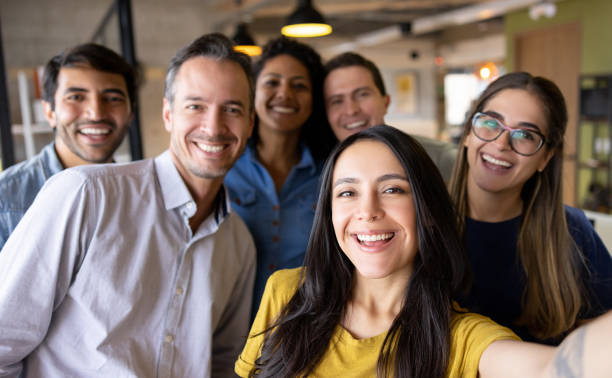
\includegraphics[width=0.8\textwidth]{foto-kelompok}\par

	\vspace{1.2cm}
	{\bfseries Disusun oleh:\par}
	\vspace{0.2cm}
	\textbf{Kelompok \nomorkelompok{} -- \namakelompok}
	\vspace{0.5cm} \\
	\begin{tabular}{l l}
		Gabriella Botimada Lubis & (13524006) \\
		Agatha Tatianingseto & (13524008) \\
		Muhammad Nur Majiid & (13524028) \\
		Athilla Zaidan Zidna Fann & (13524068) \\
		Reva Natania Sitohang & (13524098) \\
	\end{tabular}

	\vfill
	Program Studi Teknik Informatika\par
	Sekolah Teknik Elektro dan Informatika\par
	Institut Teknologi Bandung\par
	2026\par
\end{titlepage}


	\clearpage
	\pagenumbering{roman}
	\tableofcontents
	\listoffigures
	\listoftables
	\clearpage
	\pagenumbering{arabic}

	% Struktur mengikuti komponen laporan pada spesifikasi Tugas Besar 2
	\chapter{Deskripsi Persoalan}
	% Bab 1: Deskripsi Persoalan -- pemahaman terhadap persoalan dan dataset
\section{Latar Belakang}
\label{sec:latar-belakang}

\todo{Jelaskan konteks persoalan: penginapan ingin mengestimasi pemesanan yang akan dibatalkan
agar perencanaan kapasitas lebih akurat. Mengapa dipilih pembelajaran mesin klasik
(tanpa \textit{deep learning}) dan mengapa ini dirumuskan sebagai klasifikasi biner \cite{slide-intro}.}

\section{Rumusan Persoalan}
\label{sec:rumusan-persoalan}

\todo{Rumuskan tugas: diberikan fitur sebuah pemesanan, prediksi apakah pemesanan tersebut
dibatalkan (target). Sebutkan lima algoritma yang diimplementasikan \textit{from scratch}
(KNN, DTL, \textit{Logistic Regression}, SVM, \textit{Naive Bayes}) dan pembandingnya dari
\textit{scikit-learn}.}

\begingroup\emergencystretch=3em
\section{Deskripsi Dataset}
\label{sec:dataset}

Dataset berasal dari kompetisi Kaggle Tugas Besar 2 IF3170 (\url{https://www.kaggle.com/competitions/T2-IF3170-2026-2027}) dan berisi catatan pemesanan sebuah penginapan. Setiap baris adalah satu pemesanan, yang dicirikan oleh tamu, masa menginap, kanal pemesanan, dan harga. Tersedia tiga berkas:
\begin{itemize}
	\item \texttt{train.csv}: 27.373 baris dan 19 kolom (kolom \texttt{id}, 17 fitur, dan target \texttt{is\_canceled});
	\item \texttt{test.csv}: 6.844 baris dan 18 kolom (tanpa target);
	\item \texttt{sample\_\allowbreak submission.csv}: contoh format \textit{submission} berisi kolom \texttt{id} dan \texttt{is\_canceled}.
\end{itemize}
Kolom \texttt{id} adalah pengenal unik pesanan dan bukan fitur. Kolom ini harus dibaca sebagai teks, karena sebagian nilainya hanya berisi angka atau menyerupai notasi ilmiah (misalnya \texttt{123e4567}) dan akan rusak jika dibaca sebagai angka. Target adalah \texttt{is\_canceled}, yang hanya ada pada data latih.

\subsection{Deskripsi Fitur}
\label{subsec:deskripsi-fitur}

Dari 17 fitur, 14 bertipe numerik dan 3 kategorikal. Fitur dikelompokkan menurut tipenya pada Tabel~\ref{tab:fitur}. Kolom hitungan bertipe desimal pada data karena memuat nilai kosong. Kolom ``Kosong'' menunjukkan persentase nilai hilang pada data latih. Fitur yang tidak tercantum tidak memiliki nilai hilang. IDR adalah mata uang Rupiah.

\begin{longtable}{p{3.8cm} p{2.1cm} p{5.6cm} c}
	\caption{Deskripsi fitur dataset}\label{tab:fitur}\\
	\toprule
	\textbf{Fitur} & \textbf{Tipe} & \textbf{Deskripsi} & \textbf{Kosong} \\
	\midrule
	\endfirsthead
	\toprule
	\textbf{Fitur} & \textbf{Tipe} & \textbf{Deskripsi} & \textbf{Kosong} \\
	\midrule
	\endhead
	\texttt{days\_\allowbreak before\_\allowbreak arrival} & Kontinu & Selisih hari antara tanggal pemesanan dan kedatangan (\textit{lead time}); rentang 0--448 & 4,10\% \\
	\texttt{nightly\_\allowbreak rate\_\allowbreak idr} & Kontinu & Harga rata-rata per kamar per malam (IDR); 0 berarti menginap gratis (\textit{complimentary}); maksimum sekitar 9,2 juta & 7,45\% \\
	\midrule
	\texttt{num\_adults} & Hitungan & Jumlah tamu dewasa & 2,96\% \\
	\texttt{num\_children} & Hitungan & Jumlah tamu anak & 11,09\% \\
	\texttt{weekend\_\allowbreak nights} & Hitungan & Jumlah malam akhir pekan (Sabtu atau Minggu) & -- \\
	\texttt{weekday\_\allowbreak nights} & Hitungan & Jumlah malam hari kerja (Senin sampai Jumat) & -- \\
	\texttt{prior\_\allowbreak cancellations} & Hitungan & Jumlah pemesanan sebelumnya yang dibatalkan & -- \\
	\texttt{prior\_\allowbreak completed\_\allowbreak bookings} & Hitungan & Jumlah pemesanan sebelumnya yang tidak dibatalkan & -- \\
	\texttt{special\_\allowbreak requests} & Hitungan & Jumlah permintaan khusus (misalnya lantai tinggi atau pemandangan tertentu) & 9,13\% \\
	\midrule
	\texttt{needs\_\allowbreak parking} & Biner & 1 jika tamu membutuhkan tempat parkir mobil & 3,95\% \\
	\texttt{is\_\allowbreak returning\_\allowbreak guest} & Biner & 1 jika tamu pernah menginap sebelumnya & -- \\
	\midrule
	\texttt{meal\_package} & Kategorikal & \textit{Room Only}, \textit{Breakfast}, \textit{Half Board} (sarapan dan satu waktu makan lain), atau \textit{Full Board} (tiga kali makan sehari) & 6,43\% \\
	\texttt{room\_\allowbreak category} & Kategorikal & Tipe kamar (Type A sampai Type G); huruf dianonimkan sehingga tidak menunjukkan urutan atau kualitas & 3,66\% \\
	\texttt{booking\_\allowbreak channel} & Kategorikal & Kanal pemesanan: \textit{Online Travel Agent}, \textit{Offline Agent}, \textit{Corporate}, \textit{Airline}, atau \textit{Complimentary} & -- \\
	\midrule
	\texttt{arrival\_year} & Tanggal & Tahun kedatangan (2023 atau 2024) & -- \\
	\texttt{arrival\_\allowbreak month} & Tanggal & Bulan kedatangan (1--12) & -- \\
	\texttt{arrival\_day} & Tanggal & Tanggal kedatangan (1--31) & -- \\
	\bottomrule
\end{longtable}

Tiga hal dari tabel ini penting bagi tahap berikutnya. Pertama, skala fitur sangat timpang, dari 0--1 pada fitur biner hingga jutaan pada \texttt{nightly\_\allowbreak rate\_\allowbreak idr}. Kedua, \texttt{room\_\allowbreak category} dan sebagian nilai \texttt{meal\_package} adalah label tanpa urutan sehingga tidak boleh dikodekan sebagai bilangan berurutan. Ketiga, tanggal kedatangan tersebar pada tiga kolom, yang dapat digabung menjadi periode kedatangan (Subbab~\ref{subsec:eda-waktu}).

\subsection{Variabel Target}
\label{subsec:target}

Target \texttt{is\_canceled} bernilai 1 jika pemesanan dibatalkan dan 0 jika tidak. Pada data latih, 32,8\% pesanan dibatalkan, yaitu kelas tidak batal 18.404 baris (67,2\%) berbanding kelas batal 8.969 baris (32,8\%), dengan rasio sekitar 2,05 : 1. Ketidakseimbangan ini moderat, bukan ekstrem.

Ketidakseimbangan ini memengaruhi pemilihan metrik. Model yang selalu memprediksi ``tidak batal'' mencapai \textit{accuracy} 0,6723, yang tampak tinggi, tetapi \textit{Macro F1}-nya hanya 0,4020 dan sama sekali tidak berguna bagi penginapan karena tidak pernah menemukan pesanan yang batal. Karena itu \textit{accuracy} saja tidak cukup dan metrik utama yang dipakai adalah \textit{Macro F1} (Subbab~\ref{sec:metrik}).

\begin{figure}[H]
	\centering
	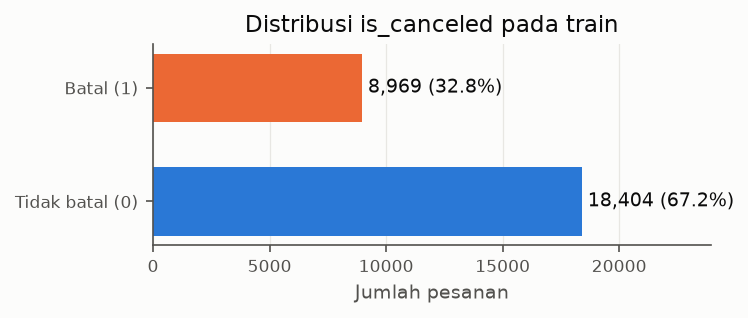
\includegraphics[width=0.6\textwidth]{target_distribution.png}
	\caption{Distribusi kelas target pada data latih}
	\label{fig:target-distribution}
\end{figure}
\endgroup

\begingroup\emergencystretch=3em
\section{Eksplorasi Data}
\label{sec:eda}

Eksplorasi data (\textit{exploratory data analysis}, EDA) dilakukan pada data latih di \texttt{src/kaggle/eda.ipynb}, dan seluruh gambar tersimpan di \texttt{output/eda/}. Tujuannya memahami struktur, kualitas, dan pola data sebelum algoritma dibangun, sehingga keputusan \textit{cleaning} dan \textit{preprocessing} pada tiap algoritma didukung bukti. Data latih dan data uji tidak pernah digabung; data uji hanya dipakai untuk membandingkan distribusi dan kualitasnya.

\subsection{Kualitas Data}
\label{subsec:kualitas-data}

\paragraph{Nilai hilang.} Delapan kolom memiliki nilai kosong sebesar 2,96\% sampai 11,09\% (Gambar~\ref{fig:missing-pct}), dengan pola yang hampir sama pada data uji. Hanya 60,8\% baris yang lengkap: 8.478 baris kehilangan satu kolom, 1.933 baris dua kolom, dan sisanya tiga sampai lima kolom. Menghapus baris yang tidak lengkap akan membuang 39,2\% data, dan cara itu tidak dapat diterapkan pada data uji karena semua barisnya harus diprediksi. Imputasi karena itu wajib.

Hubungan kekosongan dengan target diuji dengan uji \textit{chi-square} antara indikator ``kosong'' dan target, dengan koreksi Bonferroni. Hanya \texttt{special\_\allowbreak requests} yang kekosongannya berkaitan dengan target: tingkat batal 40,8\% saat kosong dan 31,9\% saat terisi. Tujuh kolom lain tidak signifikan, sehingga imputasi sederhana memadai untuk kolom tersebut. Kekosongan \texttt{special\_\allowbreak requests} condong ke nilai nol: pada kanal \textit{Online Travel Agent}, tingkat batal baris kosong menyiratkan sekitar 83\% di antaranya bernilai nol, padahal hanya 36,6\% baris terisi yang bernilai nol. Imputasi dengan median (yaitu 0) sesuai dengan nilai yang paling mungkin, dan indikator kosong dapat ditambahkan sebagai fitur.

\begin{figure}[H]
	\centering
	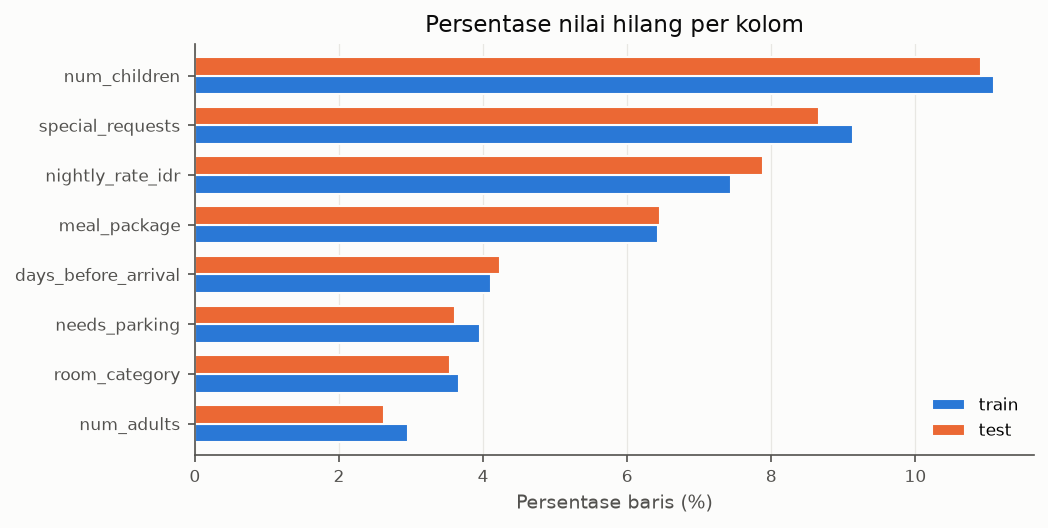
\includegraphics[width=0.75\textwidth]{missing_pct.png}
	\caption{Persentase nilai hilang per fitur pada data latih dan data uji}
	\label{fig:missing-pct}
\end{figure}

\paragraph{Duplikat.} Kolom \texttt{id} selalu unik, sehingga duplikat diperiksa pada seluruh fitur. Terdapat 62 grup duplikat dengan 66 baris berlebih, dan 2 grup memiliki label yang berbeda. Membuang duplikat identik beserta labelnya menghapus 64 baris (0,2\%), sehingga dampaknya kecil. Selain itu, 42 baris data uji memiliki fitur yang sama dengan baris data latih. Baris uji tersebut tetap harus diprediksi dan tidak boleh dihapus.

\paragraph{Nilai tidak wajar.} Beberapa kombinasi nilai tampak tidak masuk akal, tetapi ternyata informatif dan juga muncul pada data uji, sehingga tidak dihapus (Tabel~\ref{tab:anomali}). Sebagai contoh, \texttt{num\_adults} $=0$ bukan kesalahan data, karena 105 dari 106 baris memiliki anak dan satu sisanya kosong. Tarif nol hampir selalu tidak batal (0,7\%); dari 413 barisnya, 267 berasal dari kanal \textit{Complimentary} (tidak pernah batal) dan 146 dari \textit{Online Travel Agent} (2,1\% batal). Median tarif kanal \textit{Complimentary} adalah 0 sedangkan median keseluruhan 1,644 juta, sehingga imputasi tarif dengan median global akan keliru pada kanal ini dan imputasi per kanal lebih tepat. Kolom \texttt{is\_\allowbreak returning\_\allowbreak guest} juga sepenuhnya konsisten dengan riwayat pesanan sebelumnya. Hanya \texttt{num\_children} $\ge 9$ dan tarif di atas 6 juta yang layak dipangkas, masing-masing 3 baris dan tidak ada pada data uji.

\begin{table}[H]
	\centering
	\caption{Nilai tidak wajar pada data latih dan data uji}
	\label{tab:anomali}
	\begin{tabular}{l r c r}
		\toprule
		\textbf{Aturan} & \textbf{Baris latih} & \textbf{Tingkat batal} & \textbf{Baris uji} \\
		\midrule
		\texttt{num\_adults} $= 0$ & 106 & 0,302 & 22 \\
		total malam $= 0$ & 64 & 0,031 & 9 \\
		\texttt{nightly\_\allowbreak rate\_\allowbreak idr} $= 0$ & 413 & 0,007 & 85 \\
		\texttt{num\_children} $\ge 9$ & 3 & 0,333 & 0 \\
		\texttt{prior\_\allowbreak cancellations} $\ge 10$ & 21 & 0,095 & 8 \\
		total malam $\ge 15$ & 55 & 0,800 & 12 \\
		tarif $> 6$ juta & 3 & 0,667 & 0 \\
		\bottomrule
	\end{tabular}
\end{table}

\subsection{Distribusi Fitur Numerik}
\label{subsec:eda-numerik}

\paragraph{Fitur kontinu.} \texttt{days\_\allowbreak before\_\allowbreak arrival} adalah fitur terkuat. Tingkat batal naik dari 8,5\% pada desil terendah (0 sampai 4 hari) ke 75,7\% pada desil tertinggi (di atas 213 hari), dengan lompatan tajam dari 36,3\% ke 68,0\% di sekitar 151 hari. Hubungan ini monotonik tetapi tidak linear. Sebaliknya, \texttt{nightly\_\allowbreak rate\_\allowbreak idr} tidak monotonik: tingkat batal naik sampai puncak 47,5\% pada tarif sekitar 1,8 sampai 1,9 juta, lalu turun lagi, sedangkan tarif nol membentuk kelompok tersendiri yang hampir tidak pernah batal. Model linear tidak dapat menangkap bentuk ini tanpa transformasi fitur.

\begin{figure}[H]
	\centering
	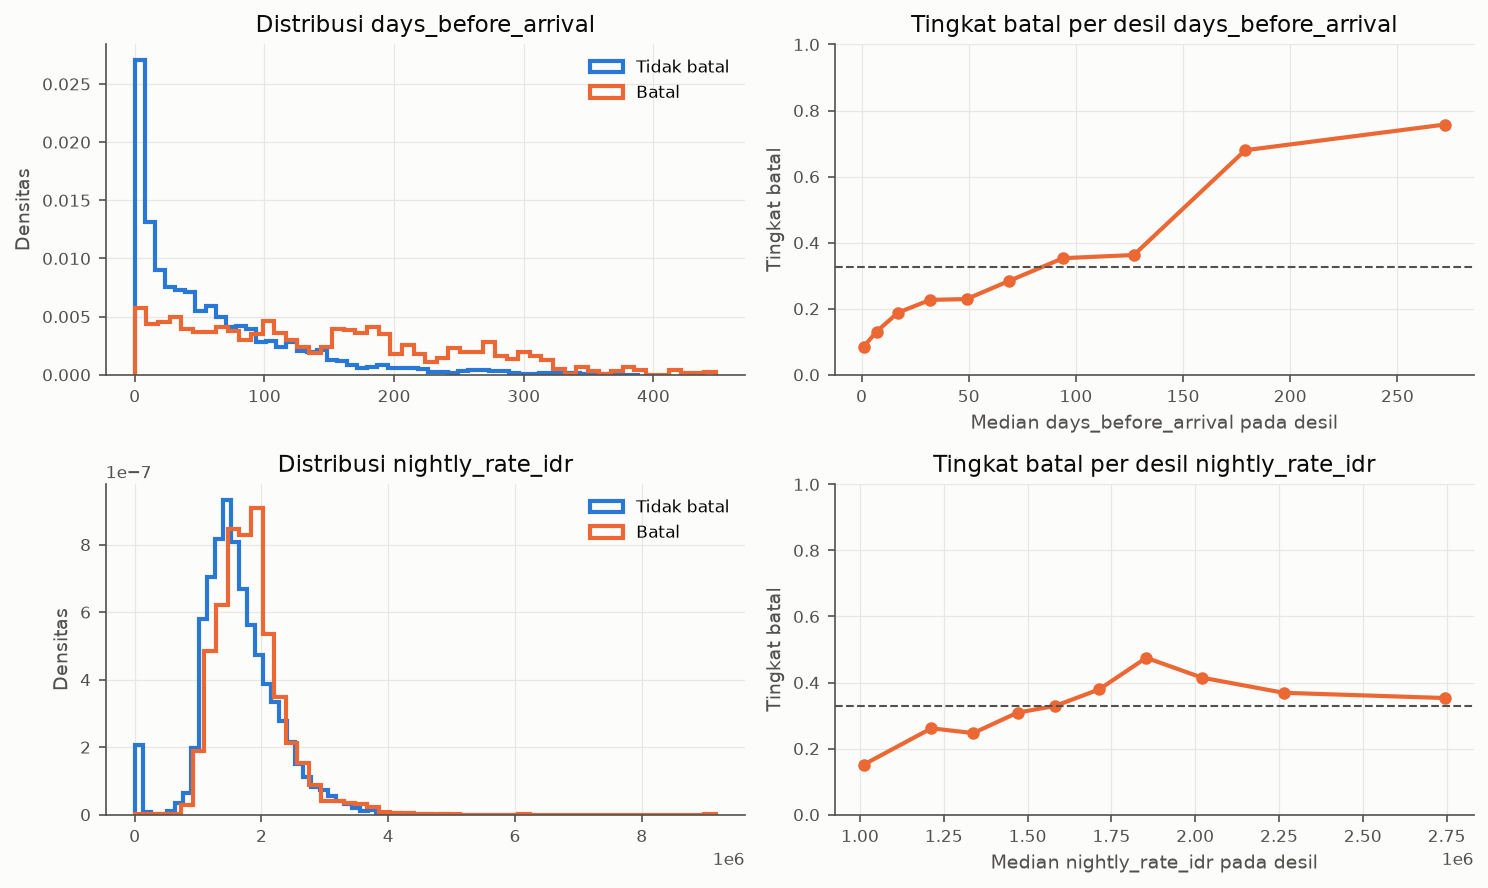
\includegraphics[width=0.9\textwidth]{continuous_features.png}
	\caption{Distribusi fitur kontinu menurut kelas target (kiri) dan tingkat batal per desil (kanan)}
	\label{fig:continuous-features}
\end{figure}

\paragraph{Fitur hitungan dan biner.} \texttt{special\_\allowbreak requests} adalah sinyal negatif terkuat: tingkat batal turun dari 43,2\% pada nilai 0 ke 23,8\% dan 14,3\% pada nilai 1 dan 2, lalu 0\% untuk seluruh 563 baris dengan nilai minimal 3. Tamu lama (1,5\% batal), kebutuhan parkir (10,1\%), dan riwayat pembatalan cenderung menurunkan risiko, sedangkan masa inap panjang cenderung menaikkannya. \texttt{num\_adults} dan \texttt{num\_children} lemah.

\subsection{Distribusi Fitur Kategorikal}
\label{subsec:eda-kategorikal}

Ketiga fitur kategorikal berhubungan signifikan dengan target menurut uji \textit{chi-square} ($p < 10^{-7}$), tetapi kekuatannya berbeda (Gambar~\ref{fig:categorical-rates}). \texttt{booking\_\allowbreak channel} paling kuat: kanal \textit{Complimentary} tidak pernah batal, \textit{Corporate} 11,5\%, dan \textit{Online Travel Agent} 36,4\%. Pada \texttt{meal\_package}, \textit{Half Board} menonjol dengan 45,9\%. \texttt{room\_\allowbreak category} paling lemah. Beberapa kategori sangat langka: \textit{Full Board} hanya 4 baris dan Type E hanya 7 baris pada data latih (tidak ada Type E pada data uji), sehingga \textit{one-hot encoding} akan menghasilkan kolom yang hampir selalu nol dan kategori langka perlu digabung. Baris kosong pada kedua kolom itu memiliki tingkat batal mendekati rata-rata, sehingga cukup diberi kategori sendiri. Tidak ada kategori baru pada data uji.

\begin{figure}[H]
	\centering
	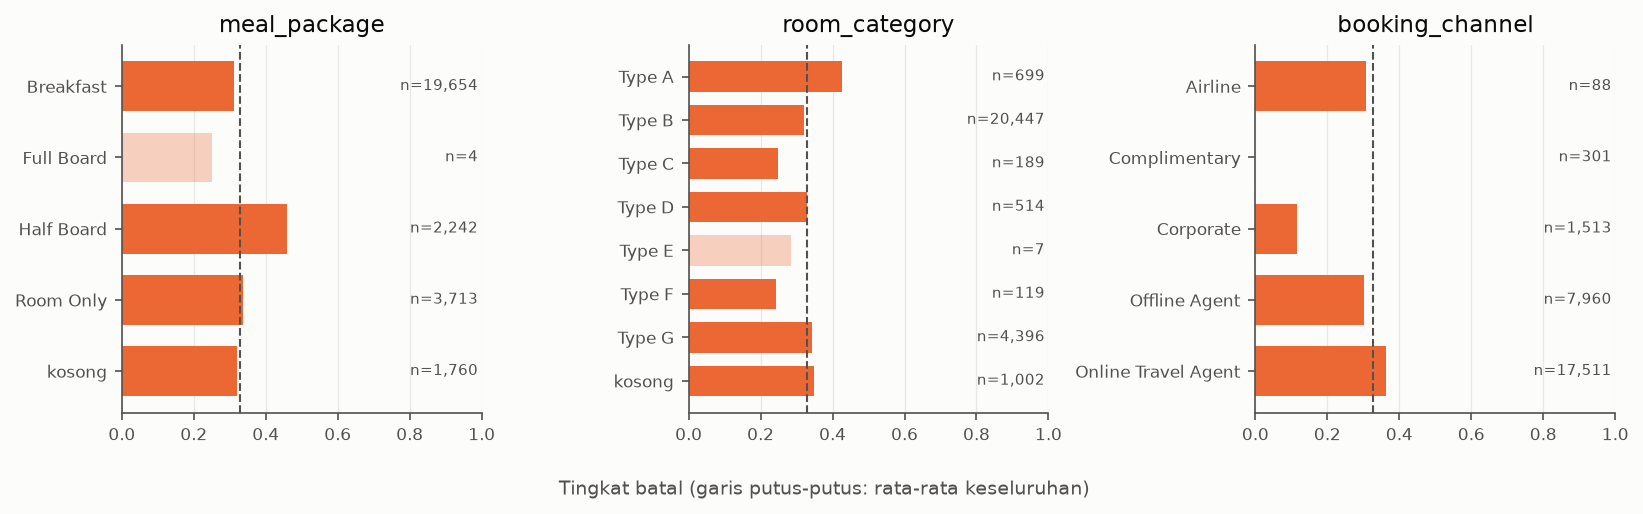
\includegraphics[width=\textwidth]{categorical_rates.png}
	\caption{Tingkat pembatalan per kategori (garis putus-putus: rata-rata keseluruhan; $n$ pada tiap batang)}
	\label{fig:categorical-rates}
\end{figure}

\subsection{Pola Waktu}
\label{subsec:eda-waktu}

Data latih dan data uji mencakup rentang tanggal kedatangan yang sama (1 Juli 2023 sampai 30 Desember 2024), dan porsi data uji per bulan stabil pada 19,0\% sampai 22,8\%. Artinya pembagian data bersifat acak, bukan berdasarkan waktu, sehingga \textit{stratified k-fold} mewakili kondisi data uji pada Kaggle.

Periode kedatangan membawa sinyal yang besar (Gambar~\ref{fig:monthly-trend}). Tingkat batal bergerak dari 2,5\% pada Desember 2023 hingga 64,2\% pada Juli 2023, walaupun Juli 2023 hanya memuat 274 baris. Pola ini bukan musiman murni: Oktober bernilai 16,2\% pada 2023 dan 46,5\% pada 2024, sedangkan Juli bernilai 64,2\% dan 42,0\%. Karena itu \texttt{arrival\_\allowbreak month} saja tidak cukup, dan kombinasi tahun dan bulan lebih informatif. Hari kedatangan (30,5\% sampai 37,2\%) dan tanggal (26,8\% sampai 40,7\%) jauh lebih lemah. Efek \textit{lead time} juga bergantung pada periode: \textit{lead time} 151 sampai 250 hari memiliki tingkat batal 0,72 sampai 0,82 pada Mei hingga Oktober 2024, tetapi hanya 0,38 pada Desember 2024.

Bulan pemesanan dapat diturunkan dari tanggal kedatangan dikurangi \texttt{days\_\allowbreak before\_\allowbreak arrival}. Fitur ini diketahui saat pesanan dibuat, sehingga tidak membocorkan target, dan memiliki sinyal yang tidak identik dengan bulan kedatangan (misalnya lompatan dari 17,3\% pada September 2023 ke 45,1\% pada Oktober 2023). Penurunan hingga 0,3\% pada Desember 2024 perlu dibaca hati-hati: seluruh kedatangan berakhir pada Desember 2024, sehingga pesanan pada bulan itu pasti berlead time pendek, yang memang jarang batal.

Satu catatan penting: fitur periode efektif untuk Kaggle karena data uji berada pada periode yang sama dengan data latih, tetapi tidak akan berlaku untuk bulan yang belum pernah terlihat pada penerapan nyata.

\begin{figure}[H]
	\centering
	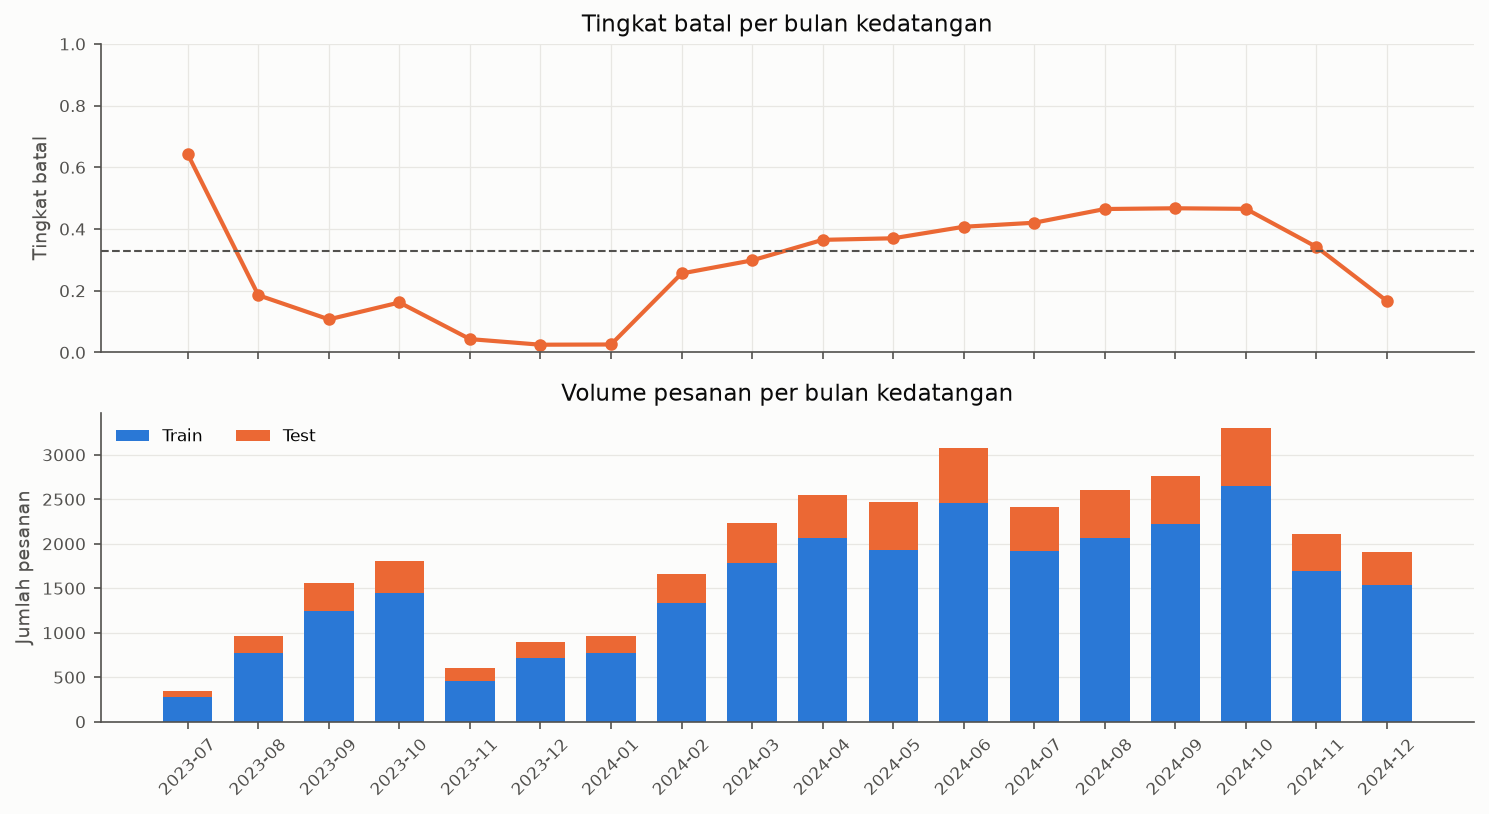
\includegraphics[width=0.9\textwidth]{monthly_trend.png}
	\caption{Tingkat pembatalan (atas) dan volume pesanan (bawah) per bulan kedatangan}
	\label{fig:monthly-trend}
\end{figure}

\subsection{Korelasi dan Relevansi Fitur}
\label{subsec:eda-korelasi}

Korelasi Spearman dipilih karena banyak fitur miring dan berupa hitungan. Korelasi terhadap target terkuat dimiliki \texttt{days\_\allowbreak before\_\allowbreak arrival} (0,418) dan \texttt{special\_\allowbreak requests} ($-0{,}261$), disusul \texttt{arrival\_year} (0,180) dan \texttt{nightly\_\allowbreak rate\_\allowbreak idr} (0,148). Redundansi utama hanya satu kelompok, yaitu riwayat tamu: \texttt{prior\_\allowbreak completed\_\allowbreak bookings} dengan \texttt{is\_\allowbreak returning\_\allowbreak guest} (0,932) dan \texttt{prior\_\allowbreak cancellations} dengan \texttt{is\_\allowbreak returning\_\allowbreak guest} (0,587). Pasangan fitur lain tidak berkorelasi tinggi.

Korelasi hanya menangkap hubungan monotonik, sehingga \textit{mutual information} (MI) ikut dihitung pada data latih setelah imputasi sementara, dan Cram\'er's V untuk fitur kategorikal. MI menempatkan \texttt{days\_\allowbreak before\_\allowbreak arrival} di puncak (0,105), diikuti \texttt{arrival\_ym}, yaitu kombinasi tahun dan bulan kedatangan (0,052), \texttt{special\_\allowbreak requests} (0,037), dan bulan pemesanan (0,028). \texttt{arrival\_ym} jauh melampaui \texttt{arrival\_\allowbreak month} (0,025) dan memiliki Cram\'er's V tertinggi (0,298), yang mendukung penggunaan kombinasi tahun-bulan. \texttt{room\_\allowbreak category} dan \texttt{num\_children} memiliki MI terendah. Ukuran ini univariat dan tidak melihat interaksi, sehingga fitur yang lemah tidak langsung dibuang; pemilihan fitur diputuskan melalui validasi silang pada tiap algoritma.

\begin{figure}[H]
	\centering
	\begin{subfigure}{0.48\textwidth}
		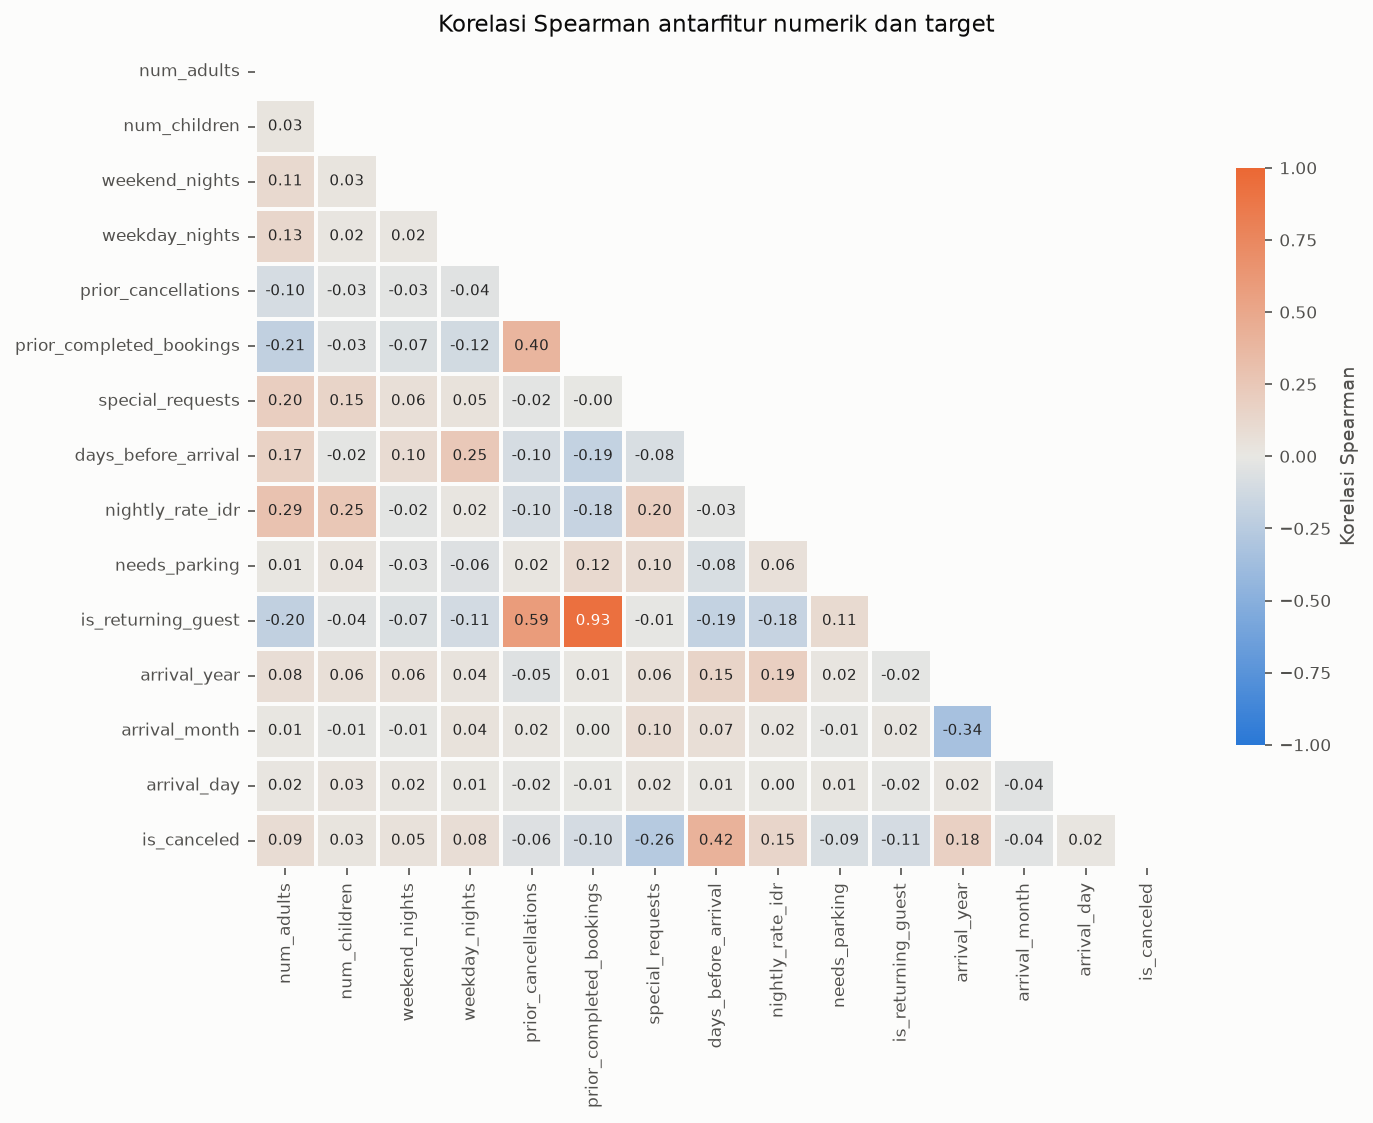
\includegraphics[width=\textwidth]{spearman_correlation.png}
		\caption{Korelasi Spearman}
	\end{subfigure}
	\hfill
	\begin{subfigure}{0.48\textwidth}
		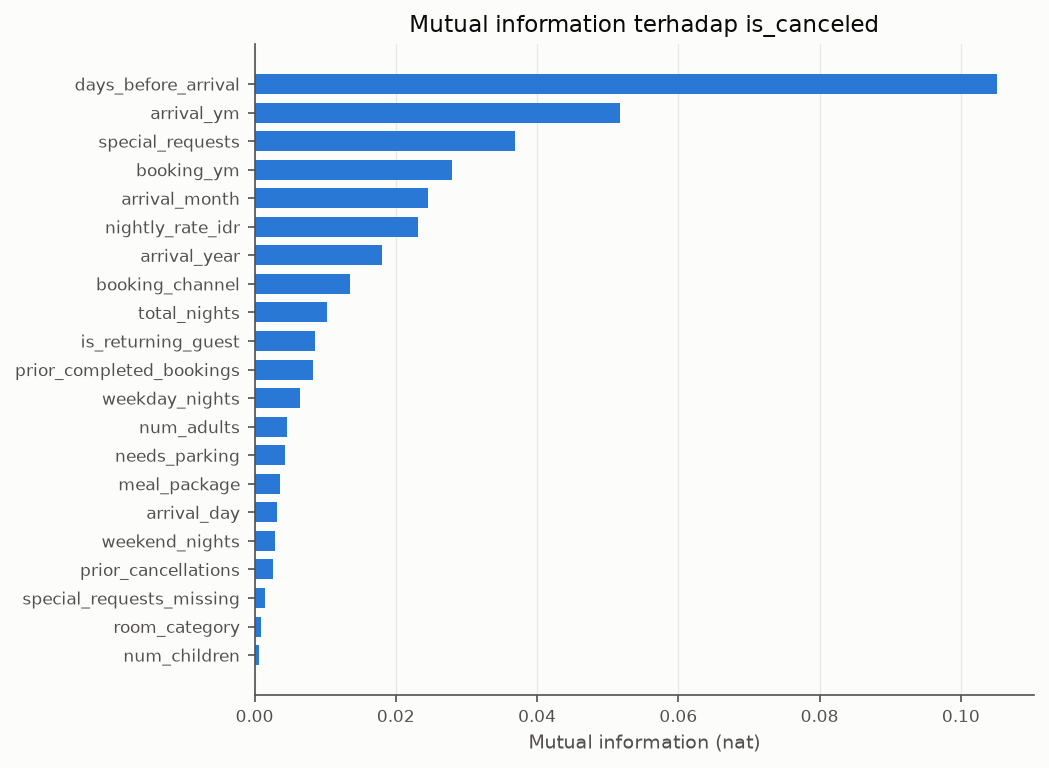
\includegraphics[width=\textwidth]{mutual_information.png}
		\caption{\textit{Mutual information}}
	\end{subfigure}
	\caption{Relevansi fitur terhadap target}
	\label{fig:relevansi-fitur}
\end{figure}

\subsection{Perbandingan Data Latih dan Data Uji}
\label{subsec:eda-train-test}

Skor validasi hanya mewakili skor data uji jika kedua berkas berasal dari distribusi yang sama. Pergeseran distribusi diukur dengan \textit{Population Stability Index} (PSI), dengan batas (\textit{bin}) dari data latih dan data uji dievaluasi pada batas tersebut sehingga kedua berkas tetap terpisah, serta statistik Kolmogorov-Smirnov (KS) untuk fitur numerik. PSI tertinggi hanya 0,0021 dan KS tertinggi 0,0149, jauh di bawah batas kestabilan 0,1, dan tidak ada kategori baru pada data uji. Tidak ada pergeseran distribusi, sehingga skor validasi silang dapat dijadikan perkiraan skor data uji.

\subsection{Ringkasan Temuan}
\label{subsec:ringkasan-eda}

EDA ini adalah tahap \textit{data understanding} pada kerangka CRISP-DM \cite{slide-crispdm}: memahami struktur, kualitas, dan pola data sebelum \textit{data preparation} dan pemodelan. Temuan utama dan keputusan yang diturunkannya dirangkum pada Tabel~\ref{tab:ringkasan-eda}, dan menjadi dasar subbab \textit{preprocessing} tiap algoritma di Bab~2. Kolom kanan adalah implikasi yang disarankan EDA; keputusan akhir tiap algoritma dibahas pada subbabnya masing-masing dan dapat berbeda karena kebutuhan algoritmanya.

\begin{table}[H]
	\centering
	\caption{Temuan EDA dan implikasinya untuk \textit{preprocessing}}
	\label{tab:ringkasan-eda}
	\begin{tabular}{p{6.4cm} p{6.4cm}}
		\toprule
		\textbf{Temuan} & \textbf{Implikasi untuk \textit{preprocessing}} \\
		\midrule
		Hanya 60,8\% baris lengkap; delapan kolom memiliki nilai hilang & Imputasi (median untuk numerik, kategori sendiri untuk kategorikal), bukan hapus baris \\
		Kekosongan \texttt{special\_\allowbreak requests} berkaitan dengan target & Tambahkan indikator kosong \\
		Tarif nol hampir semuanya kanal \textit{Complimentary}; median tarif per kanal berbeda & Imputasi tarif per kanal lebih tepat daripada median global \\
		64 baris duplikat identik (0,2\%) & Buang duplikat pada data latih saja, data uji tidak disentuh \\
		Nilai ekstrem informatif dan muncul juga pada data uji & Tidak dihapus; pangkas hanya tiga baris ekstrem \\
		\texttt{days\_\allowbreak before\_\allowbreak arrival} dan \texttt{nightly\_\allowbreak rate\_\allowbreak idr} berhubungan nonlinear dengan target & Transformasi (misalnya logaritma) dan fitur interaksi untuk model linear \\
		Kategori sangat langka (\textit{Full Board}, Type E) & Gabungkan kategori langka sebelum \textit{one-hot} \\
		Periode kedatangan dan pemesanan membawa sinyal besar, dan data uji berada pada periode yang sama & Pakai kombinasi tahun-bulan sebagai fitur; hanya sah untuk Kaggle, bukan untuk periode baru \\
		\texttt{prior\_\allowbreak completed\_\allowbreak bookings} berkorelasi 0,932 dengan \texttt{is\_\allowbreak returning\_\allowbreak guest} & Redundan, dipertimbangkan pada \textit{feature selection} \\
		Skala fitur sangat timpang & Standardisasi, di-\textit{fit} hanya pada data latih \\
		Kelas tidak seimbang moderat (2,05 : 1) & \textit{Threshold} dipilih untuk Macro F1, tanpa \textit{resampling} \\
		Tidak ada pergeseran distribusi (PSI $< 0{,}003$) & Validasi silang mewakili skor data uji \\
		\bottomrule
	\end{tabular}
\end{table}
\endgroup

\section{Metrik Evaluasi}
\label{sec:metrik}

\paragraph{Metrik utama: \textit{Macro F1}.} Kompetisi Kaggle menilai \textit{submission} dengan \textit{Macro F1-score}, yaitu rata-rata F1 kelas tidak batal dan F1 kelas batal. F1 suatu kelas adalah rata-rata harmonik \textit{precision} dan \textit{recall} kelas tersebut:
\begin{equation}
	\text{F1}_c = \frac{2 \cdot \text{Precision}_c \cdot \text{Recall}_c}{\text{Precision}_c + \text{Recall}_c},
	\qquad
	\text{Macro F1} = \frac{1}{|C|} \sum_{c \in C} \text{F1}_c,
	\label{eq:macro-f1}
\end{equation}
dengan $C = \{0, 1\}$ himpunan kelas, $\text{Precision}_c = TP_c / (TP_c + FP_c)$, dan $\text{Recall}_c = TP_c / (TP_c + FN_c)$. Kedua kelas berbobot sama pada rata-rata, tanpa memandang jumlah barisnya.

Metrik ini sesuai untuk data yang tidak seimbang (Subbab~\ref{subsec:target}) karena \textit{accuracy} dapat menyesatkan. Model yang selalu memprediksi ``tidak batal'' mencapai \textit{accuracy} 0,6723, tetapi \textit{Macro F1}-nya hanya 0,4020 karena F1 kelas batal bernilai nol; model yang selalu memprediksi ``batal'' hanya mencapai 0,2468. Nilai 0,4020 adalah \textit{baseline} yang harus dilampaui setiap model. Menurut halaman kompetisi, papan peringkat publik memakai sekitar 30\% data uji dan peringkat akhir memakai 70\% sisanya, sehingga keputusan pemilihan model didasarkan pada validasi silang pada data latih, bukan pada skor publik.

\paragraph{Metrik pendukung.} Selain \textit{Macro F1}, dilaporkan:
\begin{itemize}
	\item \textit{Accuracy}, yaitu proporsi prediksi yang benar, $(TP + TN) / n$. Dilaporkan sebagai gambaran umum, bukan sebagai dasar pemilihan model;
	\item \textit{Precision} dan \textit{recall} kelas batal. \textit{Precision} menjawab ``dari pesanan yang diprediksi batal, berapa yang benar-benar batal'', dan \textit{recall} menjawab ``dari pesanan yang batal, berapa yang berhasil ditemukan''. Keduanya penting karena memiliki konsekuensi bisnis yang berbeda (lihat di bawah);
	\item \textit{Confusion matrix}, yang menunjukkan jumlah $TN$, $FP$, $FN$, dan $TP$ sehingga jenis kesalahan model terlihat langsung;
	\item \textit{ROC-AUC}, yaitu luas di bawah kurva ROC. Metrik ini menilai kualitas peringkat peluang atau skor model tanpa bergantung pada \textit{threshold}, sehingga berguna untuk membandingkan model sebelum \textit{threshold} dipilih.
\end{itemize}

\paragraph{Validasi dan \textit{threshold}.} Model yang menghasilkan peluang (misalnya \textit{logistic regression}) mengubah peluang menjadi label dengan \textit{threshold}. \textit{Macro F1} bergantung pada \textit{threshold} ini, sehingga \textit{threshold} dipilih pada prediksi \textit{out-of-fold} dari \textit{stratified k-fold cross validation}, bukan pada data uji. Hasil pada data latih dilaporkan sebagai rata-rata dan simpangan baku antar-\textit{fold}, karena selisih antarkonfigurasi sering lebih kecil daripada variasi antar-\textit{fold} dan perlu dibaca dengan hati-hati.

\paragraph{Biaya kesalahan.} \textit{Macro F1} memperlakukan \textit{false positive} dan \textit{false negative} sama. Pada kenyataan di penginapan, keduanya tidak sama: pesanan yang diprediksi batal padahal tamu datang ($FP$) dapat menyebabkan \textit{overbooked}, sedangkan pesanan yang diprediksi datang padahal batal ($FN$) hanya menyisakan kamar kosong. Untuk bonus \textit{cost-sensitive classification}, dipakai total biaya $2 \cdot FP + 1 \cdot FN$, yang dibahas pada Bagian~\ref{sec:cost-sensitive}. Metrik ini hanya dipakai pada bagian tersebut, sedangkan perbandingan antarmodel dan \textit{submission} Kaggle tetap memakai \textit{Macro F1}.



	\chapter{Pembahasan}
	% Bab 2: Pembahasan, dibagi per algoritma.
% Setiap folder algoritma berisi: implementasi, cleaning & preprocessing, modeling & validasi,
% hasil & perbandingan sklearn, dan bonus khusus algoritma tersebut.
\section{Kerangka Umum Eksperimen}
\label{sec:kerangka-umum}

Bagian ini memuat hal yang berlaku untuk kelima algoritma: struktur kode, langkah \textit{preprocessing}
yang dipakai bersama, serta protokol validasi dan reproduksibilitas. Rincian khusus setiap algoritma
dibahas pada subbabnya masing-masing.

\subsection{Struktur Kode dan Antarmuka}

Implementasi \textit{from scratch} berada di \nolinkurl{src/algoritma/}, satu folder untuk setiap
algoritma. Notebook, skrip submisi, dan dataset Kaggle berada di \nolinkurl{src/kaggle/}. Hasil
\textit{run} (model tersimpan, berkas submisi, tabel, dan gambar) ditulis ke \nolinkurl{output/}, dan
\textit{unit test} berada di \nolinkurl{test/}.

Setiap kelas mengikuti antarmuka yang mirip dengan \textit{scikit-learn}: \texttt{fit(X, y)} untuk
melatih, \texttt{predict(X)} untuk label, dan \texttt{predict\_proba(X)} untuk peluang kelas batal,
sehingga \textit{threshold} keputusan dapat diatur di luar model. Perhitungan pada implementasi
\textit{from scratch} memakai NumPy. Satu-satunya pengecualian adalah KNN, yang memakai fungsi jarak
\texttt{cdist} dari SciPy. Pustaka lain, seperti pandas dan \textit{scikit-learn}, hanya dipakai di
notebook untuk memuat data, membuat pembagian \textit{fold}, dan menjadi pembanding.

\begin{table}[H]
	\centering
	\caption{Ringkasan implementasi algoritma}
	\label{tab:ringkasan-implementasi}
	\begin{tabularx}{\textwidth}{l l l Y}
		\toprule
		\textbf{Algoritma} & \textbf{Berkas} & \textbf{Kelas} & \textbf{Format model} \\
		\midrule
		KNN & \nolinkurl{knn/knn.py} & \texttt{KNN} & \textit{Pickle} bersama \textit{preprocessor} (\nolinkurl{output/knn/model.pkl}) \\
		DTL & \nolinkurl{dtl/} (enam modul) & \texttt{DTL} & JSON (\nolinkurl{output/dtl/dtl_model.json}) \\
		\textit{Logistic Regression} & \nolinkurl{lr/lr.py} & \texttt{LogisticRegression} & NumPy \texttt{.npz} \\
		SVM & \nolinkurl{svm/svm.py} & \texttt{SVM} & \textit{Pickle} (\nolinkurl{output/svm/svm_model.pkl}) \\
		\textit{Naive Bayes} & \nolinkurl{nb/nb.py}, \nolinkurl{nb/tan.py} & \texttt{NaiveBayes}, \texttt{TANNaiveBayes} & JSON \\
		\bottomrule
	\end{tabularx}
\end{table}

DTL, \textit{Logistic Regression}, SVM, dan \textit{Naive Bayes} menyediakan metode \texttt{save} dan
\texttt{load} di kelasnya. Model KNN disimpan dengan \textit{pickle} oleh
\nolinkurl{src/kaggle/knn_submission.py}, karena isi modelnya hanya data latih dan parameter.

\subsection{\textit{Preprocessing} Bersama}

Semua model memuat data dari \nolinkurl{src/kaggle/dataset/} dan membuang kolom \texttt{id} dari
fitur. Kolom \texttt{id} hanya dipakai untuk menulis berkas submisi. Data latih berisi 27.373 baris;
setelah duplikat dibuang tersisa 27.309 baris yang dipakai untuk pelatihan dan validasi.

Setiap algoritma memiliki \textit{preprocessing} sendiri karena kebutuhannya berbeda. KNN dan SVM
membutuhkan fitur berskala sama, DTL dapat memakai atribut kategorikal dan nilai kosong secara
langsung, sedangkan \textit{Naive Bayes} membutuhkan tipe fitur (kategorikal atau Gaussian). DTL dan
SVM memakai modul fitur yang sama, yaitu \nolinkurl{src/kaggle/booking_features.py}, yang berisi
pembersihan, fitur tanggal, imputasi beserta penanda nilai kosong, fitur ``saudara'' (pemesanan lain
yang mirip pada data latih), dan standardisasi.

Pada semua algoritma, statistik \textit{preprocessing} (rata-rata, simpangan baku, modus, kategori,
\textit{target encoding}, dan sejenisnya) hanya dihitung dari data latih, lalu diterapkan ke data
validasi dan data uji. Saat validasi silang, statistik dihitung ulang di dalam setiap \textit{fold}.
Data latih dan data uji tidak pernah digabungkan.

\subsection{Protokol Validasi dan Reproduksibilitas}

Metrik utama adalah Macro F1, sama dengan metrik kompetisi (Subbab~\ref{sec:metrik}). Validasi utama
memakai \textit{stratified} 5-\textit{fold cross validation} dengan \textit{seed} 42. DTL,
\textit{Logistic Regression}, dan \textit{Naive Bayes} menjalankannya pada seluruh data latih bersih,
sedangkan KNN menjalankannya pada data \textit{development} (data latih tanpa \textit{hold-out}). SVM
memilih kernel dan $C$ lebih dulu dengan CV 3-\textit{fold} pada sampel kecil karena biaya komputasi,
lalu merinci konfigurasi akhirnya dengan CV 5-\textit{fold}. Untuk mengurangi pengaruh satu pembagian \textit{fold}, DTL dan SVM juga mengulang
validasi dengan beberapa \textit{seed} (sepuluh \textit{seed} untuk DTL dan tujuh untuk SVM).

Untuk analisis yang membutuhkan satu model tetap, misalnya perbandingan dengan \textit{scikit-learn},
analisis kesalahan, dan \textit{cost-sensitive}, KNN, \textit{Logistic Regression}, dan SVM juga
memakai pembagian \textit{hold-out} 80:20 (21.847 baris latih dan 5.462 baris validasi). Rincian
skema validasi setiap algoritma ada pada subbab \textit{modeling} dan validasinya.

Versi pustaka dipatok di \nolinkurl{requirements.txt} (antara lain NumPy 2.5.4, pandas 3.1.1, dan
\textit{scikit-learn} 1.9.1). Submisi Kaggle akhir direproduksi oleh
\nolinkurl{src/kaggle/svm_notebook.ipynb} dan \nolinkurl{src/kaggle/dtl_notebook.ipynb}
(Bagian~\ref{sec:kaggle}).

\section{\textit{K-Nearest Neighbors} (KNN)}
\label{sec:knn}

\todo{Satu paragraf pengantar: peran KNN dalam tugas ini dan ringkasan hasil terbaiknya.}

\subsection{Implementasi \textit{From Scratch}}
\label{subsec:knn-implementasi}

\subsubsection{Landasan Teori}
\todo{Jelaskan prinsip \textit{lazy learning}, metrik jarak (Euclidean, Manhattan, Minkowski), pemilihan $k$, \textit{voting} mayoritas atau berbobot jarak, dan penanganan \textit{tie}. Acu salindia KNN \cite{slide-knn} dan \cite{cunningham2020knn}. Sertakan rumus utama dalam lingkungan \texttt{equation}/\texttt{align}.}

\subsubsection{Struktur Kelas dan Fungsi}
\todo{Deskripsikan kelas pada \texttt{src/algoritma/knn/knn.py}: \texttt{\_\_init\_\_}, \texttt{fit}, perhitungan jarak, pencarian $k$ tetangga, \texttt{predict\_proba}, \texttt{predict}, \texttt{save}, \texttt{load}. Isi tabel di bawah, satu baris per fungsi/metode.}

\begin{table}[H]
	\centering
	\caption{Deskripsi kelas dan fungsi KNN}
	\label{tab:knn-fungsi}
	\begin{tabularx}{\textwidth}{l Y}
		\toprule
		\textbf{Fungsi/Metode} & \textbf{Deskripsi} \\
		\midrule
		\texttt{nama\_fungsi} & \todo{deskripsi} \\
		\bottomrule
	\end{tabularx}
\end{table}

\subsubsection{\textit{Source Code}}
\todo{Sisipkan potongan kode inti (perhitungan jarak (vektorisasi) dan \textit{voting}) dengan makro \texttt{\textbackslash kode}, lalu jelaskan alurnya. Cek ulang nomor baris jika kode berubah.}
% \kode{../../src/algoritma/knn/knn.py}{1}{30}{Judul potongan kode}{lst:knn-inti}

\subsubsection{\textit{Save} dan \textit{Load} Model}
\todo{Format penyimpanan (JSON/\texttt{.npz}/\textit{pickle}), isi yang disimpan, dan contoh pemakaian.}

\subsection{\textit{Data Cleaning} dan \textit{Preprocessing}}
\label{subsec:knn-preprocessing}

\todo{Jelaskan \textit{pipeline} khusus KNN beserta alasan tiap langkah, dikaitkan dengan temuan EDA (Subbab~\ref{sec:eda}) dan karakteristik algoritma. Semua transformasi di-\textit{fit} pada data latih saja lalu diterapkan ke data uji \cite{slide-dataprep}.}

\subsubsection{Penanganan \textit{Missing Values}}
\todo{KNN tidak bisa menghitung jarak dengan nilai hilang, sehingga imputasi wajib. Jelaskan strategi per kolom (median/modus/konstanta) dan alasannya.}

\subsubsection{Data Duplikat dan Data Tidak Valid}
\todo{Jumlah duplikat, nilai tidak wajar, atau \textit{outlier} yang ditangani untuk KNN dan caranya. Baris data uji tidak boleh dibuang.}

\subsubsection{Konstruksi Fitur dan \textit{Encoding}}
\todo{KNN butuh fitur numerik. Jelaskan \textit{encoding} kategorikal (\textit{one-hot} vs \textit{ordinal}/\textit{target}) dan dampaknya ke jarak (dimensi besar membuat jarak kurang bermakna).}

\subsubsection{Normalisasi dan Standarisasi}
\todo{Wajib karena KNN berbasis jarak. Fitur berskala besar akan mendominasi. Jelaskan \textit{scaler} yang dipilih (standar/\textit{min-max}/\textit{robust}).}

\subsubsection{Penanganan \textit{Imbalanced Data}}
\todo{Misalnya \textit{distance-weighted voting}, \textit{threshold} probabilitas, atau \textit{resampling}.}

\subsubsection{\textit{Feature Selection}}
\todo{Sangat berpengaruh karena fitur tak relevan ikut menambah jarak (\textit{curse of dimensionality}). Sebutkan fitur akhir yang dipakai.}

\subsubsection{\textit{Dimensionality Reduction}}
\todo{Relevan untuk KNN: mengurangi dimensi dan mempercepat perhitungan jarak. Laporkan dampaknya.}

\subsection{\textit{Modeling} dan Validasi}
\label{subsec:knn-validasi}

\subsubsection{Skema Validasi}
Setelah deduplikasi, sebanyak 27.309 baris dibagi secara \textit{stratified} dengan \textit{seed} 42 menjadi \textbf{21.847 data development} (80\%) dan \textbf{5.462 data holdout} (20\%). Seluruh pemilihan fitur dan hiperparameter dilakukan pada development. Data \textit{holdout} baru digunakan setelah konfigurasi ditentukan untuk memperoleh evaluasi yang terpisah dari proses pemilihan model.

Pada development, sepuluh kandidat fitur terlebih dahulu dibandingkan dengan \textit{stratified} 3-\textit{fold} CV. Dua representasi dengan Macro F1 tertinggi kemudian diuji dengan \textit{stratified} 5-\textit{fold} CV untuk mencari hiperparameter. Dalam setiap \textit{fold}, imputasi, normalisasi, dan kategori \textit{one-hot} di-\textit{fit} pada bagian latih saja. Nilai evaluasi yang dilaporkan adalah rata-rata Macro F1 tiap \textit{fold} beserta simpangan baku sampelnya. Skema ini menghindari kebocoran statistik \textit{preprocessing} dari \textit{fold} validasi, namun pemilihan dua kandidat awal dan pencarian parameter memakai development yang sama sehingga skor CV terbaik tetap merupakan hasil pemilihan model.

\subsubsection{\textit{Hyperparameter Tuning}}
Pencarian dilakukan atas dua representasi fitur, tujuh pilihan $k$, dan tiga metrik jarak. Total terdapat \textbf{42 konfigurasi}, semuanya menggunakan suara mayoritas tanpa pembobotan jarak. Ruang pencarian ditampilkan pada Tabel~\ref{tab:knn-grid}.

\begin{table}[H]
 \centering
 \caption{Ruang pencarian hiperparameter KNN}
 \label{tab:knn-grid}
 \begin{tabularx}{\textwidth}{l Y l}
  \toprule
  \textbf{Komponen} & \textbf{Kandidat} & \textbf{Terpilih} \\
  \midrule
  Representasi & 16 atau 15 fitur hasil seleksi & 16 fitur \\
  $k$ & 3, 5, 7, 9, 11, 15, 21 & 7 \\
  Metrik jarak & Manhattan, Euclidean, Minkowski ($p=3$) & Manhattan \\
  Pembobotan suara & \textit{Uniform} (tetap) & \textit{Uniform} \\
  \bottomrule
 \end{tabularx}
\end{table}

Hasil terbaik untuk setiap pasangan representasi dan metrik ditampilkan pada Tabel~\ref{tab:knn-tuning}. Nilai dalam tabel berasal dari berkas \nolinkurl{output/knn/tuning.csv}. Pada kombinasi yang diuji, konfigurasi 16 fitur dengan Manhattan $k=7$ memberikan rata-rata Macro F1 tertinggi, yaitu 0,82126.

\begin{table}[H]
 \centering
 \caption{Konfigurasi terbaik per representasi dan metrik pada 5-\textit{fold} CV}
 \label{tab:knn-tuning}
 \begin{tabular}{c l c c c}
  \toprule
  \textbf{Fitur} & \textbf{Jarak} & $\boldsymbol{k}$ & \textbf{Macro F1} & \textbf{SD} \\
  \midrule
  16 & Manhattan & 7 & \textbf{0,82126} & 0,00714 \\
  16 & Minkowski ($p=3$) & 7 & 0,82040 & 0,00721 \\
  16 & Euclidean & 7 & 0,82015 & 0,00724 \\
  15 & Minkowski ($p=3$) & 7 & 0,82013 & 0,00671 \\
  15 & Manhattan & 5 & 0,81955 & 0,00663 \\
  15 & Euclidean & 7 & 0,81869 & 0,00669 \\
  \bottomrule
 \end{tabular}
\end{table}

\begin{figure}[H]
 \centering
 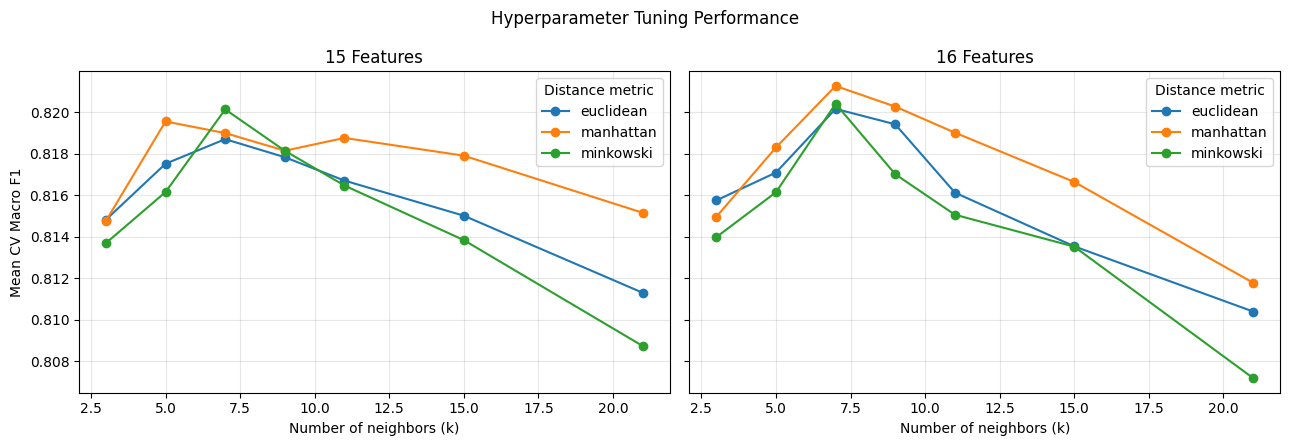
\includegraphics[width=0.94\textwidth]{knn/knn_tuning.png}
 \caption{Rata-rata Macro F1 validasi silang menurut $k$ dan metrik jarak pada dua representasi fitur}
 \label{fig:knn-tuning}
\end{figure}

Gambar~\ref{fig:knn-tuning} menunjukkan bahwa kinerja berubah ketika jumlah tetangga atau metrik jarak diganti. Perbedaan antar konfigurasi terbaik relatif kecil, yaitu 0,00086 antara Manhattan dan Minkowski pada 16 fitur. Nilai ini juga lebih kecil daripada simpangan baku antar-\textit{fold} sekitar 0,007. Oleh sebab itu, konfigurasi terbaik dipahami sebagai pilihan berdasarkan rata-rata pada ruang pencarian yang diuji, bukan bukti keunggulan yang pasti untuk semua pembagian data.

\subsubsection{Model Final}
KNN final menggunakan \textbf{16 fitur, Manhattan, $k=7$, dan suara mayoritas uniform}. Skor development CV adalah $\text{Macro F1}=0{,}82126\pm0{,}00714$, dengan \textit{accuracy} rata-rata 0,84552. Kelima skor Macro F1 per \textit{fold} adalah 0,82781, 0,81894, 0,81019, 0,82685, dan 0,82251. Model kemudian di-\textit{fit} pada seluruh development dan dievaluasi sekali pada \textit{holdout}, sebagaimana dibahas pada Subbab~\ref{subsec:knn-hasil}.

Untuk membuat prediksi data uji, konfigurasi yang sama di-\textit{fit} ulang pada \textbf{27.309 data latih bersih}. Pipeline menyimpan model dan statistik \textit{preprocessing} di \nolinkurl{output/knn/model.pkl}, hasil pencarian di \nolinkurl{output/knn/tuning.csv}, dan prediksi \textbf{6.844 baris} di \nolinkurl{output/knn/submission.csv}. Artefak tersebut dapat direproduksi melalui \nolinkurl{src/kaggle/knn_notebook.ipynb} atau \nolinkurl{src/kaggle/knn_submission.py}.
\subsection{Hasil dan Perbandingan dengan \textit{Scikit-learn}}
\label{subsec:knn-hasil}

Model terpilih dibandingkan dengan \texttt{sklearn.neighbors.KNeighborsClassifier} \cite{pedregosa2011sklearn} pada \textbf{data holdout yang sama}. Kedua implementasi menerima matriks 26 kolom yang sama dari \textit{preprocessor} yang hanya di-\textit{fit} pada development. Parameter pembanding disamakan, yaitu $k=7$, Manhattan, bobot \textit{uniform}, dan pencarian \textit{brute force}. Dengan demikian, pengujian memeriksa konsistensi hasil prediksi implementasi \textit{from scratch}, bukan perbedaan akibat pemrosesan data.

\begin{table}[H]
 \centering
 \caption{Perbandingan performa KNN pada 5.462 reservasi \textit{holdout}}
 \label{tab:knn-hasil}
 \begin{tabular}{l c c c c}
  \toprule
  \textbf{Implementasi} & \textbf{Macro F1} & \textbf{Accuracy} & \textbf{Macro Precision} & \textbf{Macro Recall} \\
  \midrule
  \textit{From scratch} & 0,82830 & 0,85244 & 0,83803 & 0,82075 \\
  \textit{Scikit-learn} & 0,82830 & 0,85244 & 0,83803 & 0,82075 \\
  \bottomrule
 \end{tabular}
\end{table}

\textbf{Seluruh 5.462 prediksi identik} antara kedua implementasi, sehingga kesesuaian label mencapai 100\%. Confusion matrix keduanya sama, sebagaimana ditampilkan pada Gambar~\ref{fig:knn-cm}. Hasil ini mendukung ketepatan implementasi jarak dan suara mayoritas pada konfigurasi serta data yang diuji. Kesamaan prediksi tersebut tidak berarti seluruh kemungkinan \textit{tie} jarak akan selalu ditangani identik oleh kedua implementasi.

\begin{figure}[H]
 \centering
 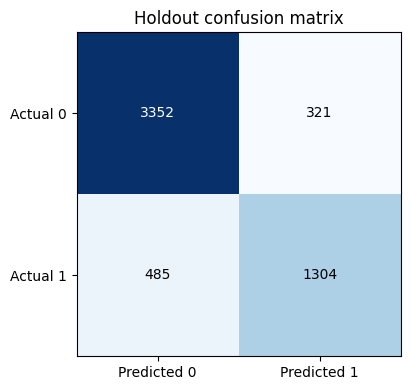
\includegraphics[width=0.66\textwidth]{knn/knn_confusion_matrix.png}
 \caption{\textit{Confusion matrix} KNN \textit{from scratch} pada \textit{holdout}, identik dengan \textit{scikit-learn}}
 \label{fig:knn-cm}
\end{figure}

\subsubsection{Analisis}
Dari 3.673 reservasi yang sebenarnya tidak dibatalkan, model mengklasifikasikan 3.352 dengan benar dan menghasilkan 321 \textit{false positive}. Dari 1.789 reservasi yang dibatalkan, model mengenali 1.304 dengan benar dan melewatkan 485 sebagai \textit{false negative}. \textit{Recall} kelas batal sebesar 0,72890 lebih rendah daripada kelas tidak batal sebesar 0,91261. Dengan demikian, kelemahan utama KNN pada \textit{holdout} adalah pembatalan yang tidak terdeteksi, bukan ketidakcocokan implementasi dengan pustaka.

Skor Macro F1 \textit{holdout} sebesar 0,82830 sedikit di atas rata-rata CV development 0,82126. Keduanya berada pada kisaran yang sebanding, meskipun berasal dari skema evaluasi berbeda. Peningkatan kemampuan mengenali kelas batal berpotensi dilakukan melalui kalibrasi ambang keputusan atau pembobotan fitur, tetapi perubahan tersebut tidak diterapkan pada model utama. Dalam konteks bonus biaya kesalahan, FP justru memiliki konsekuensi lebih mahal sehingga arah penyesuaian keputusan juga berbeda, seperti dibahas pada Subbab~\ref{subsec:knn-bonus}.

Pengukuran waktu prediksi tidak dilakukan sebagai eksperimen pembanding, sehingga tidak ditarik kesimpulan mengenai kecepatan kedua implementasi. Versi \textit{from scratch} memakai \texttt{cdist} dan \texttt{argpartition} dengan \textit{batch} untuk membatasi memori sementara. Pembanding \textit{scikit-learn} secara eksplisit memakai \textit{brute force} agar metode pencarian tetangganya sebanding.
\subsection{Analisis \textit{Cost-Sensitive Classification} pada KNN}
\label{subsec:knn-bonus}

Bonus \textit{cost-sensitive classification} pada spesifikasi menetapkan bahwa \textit{false positive} (FP) dua kali lebih mahal dibandingkan \textit{false negative} (FN). Dalam kasus reservasi, FP berarti model memprediksi pembatalan padahal tamu tetap datang, sehingga keputusan menjual ulang kamar dapat menimbulkan \textit{overbooking}. Konsekuensinya, penanganan klasifikasi perlu lebih berhati-hati dalam memberikan label batal. Asumsi biaya yang sama juga dibahas pada tingkat kelompok di Subbab~\ref{sec:cost-sensitive}.

\subsubsection{Perubahan Aturan Keputusan}
Dengan biaya prediksi benar nol, $C_{FP}=2$, dan $C_{FN}=1$, total biaya kesalahan didefinisikan sebagai
\begin{equation}
 C_{\mathrm{total}} = 2FP + FN.
 \label{eq:knn-cost}
\end{equation}
Jika $p$ merupakan estimasi peluang kelas batal, biaya harapan ketika memilih kelas batal adalah $2(1-p)$, sedangkan ketika memilih kelas tidak batal adalah $p$. Aturan yang meminimalkan biaya harapan memilih batal jika
\begin{equation}
 2(1-p)\le p \quad\Longleftrightarrow\quad p\ge\frac{2}{3}.
 \label{eq:knn-threshold}
\end{equation}
Pada KNN, nilai $p$ diestimasi dari proporsi suara tetangga melalui \texttt{predict\_proba}. Untuk $k=7$, aturan mayoritas biasa memerlukan sedikitnya empat tetangga berlabel batal. Ambang $2/3$ mengubah syarat tersebut menjadi \textbf{minimal lima tetangga}. Proporsi suara KNN belum dikalibrasi sebagai probabilitas, sehingga rumus ini dipakai sebagai kebijakan berbasis asumsi biaya yang kemudian diperiksa secara empiris, bukan sebagai jaminan optimum global \cite{elkan2001cost}.

\subsubsection{Hasil dan Analisis}
Simulasi dilakukan pada \textit{holdout} berukuran 5.462 menggunakan konfigurasi 16 fitur, Manhattan, dan $k=7$ yang sama dengan model utama. KNN di-\textit{fit} hanya pada development. Aturan baru diterapkan pada proporsi suara kelas batal tanpa mengubah data latih, hasil \textit{feature selection}, maupun berkas submisi.

\begin{table}[H]
 \centering
 \caption{Perbandingan keputusan KNN standar dan \textit{cost-sensitive} pada \textit{holdout}}
 \label{tab:knn-cost}
 \begin{tabular}{l r r r c}
  \toprule
  \textbf{Aturan keputusan} & \textbf{FP} & \textbf{FN} & \textbf{Total biaya} & \textbf{Macro F1} \\
  \midrule
  Mayoritas standar, minimal 4/7 & 321 & 485 & 1.127 & 0,82830 \\
  \textit{Cost-sensitive}, minimal 5/7 & 177 & 673 & \textbf{1.027} & 0,80791 \\
  \bottomrule
 \end{tabular}
\end{table}

\begin{figure}[H]
 \centering
 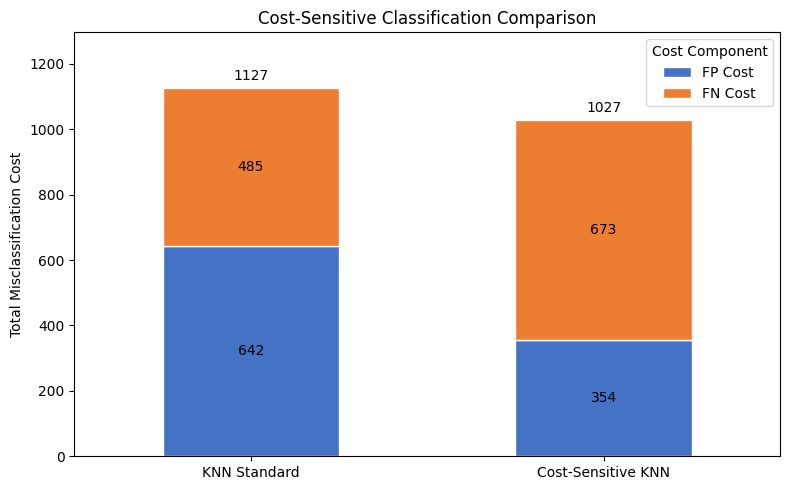
\includegraphics[width=0.72\textwidth]{knn/knn_cost_sensitive.png}
 \caption{Komponen biaya FP dan FN pada aturan mayoritas standar dan \textit{cost-sensitive}}
 \label{fig:knn-cost}
\end{figure}

Perubahan ambang mengurangi FP sebanyak 144 tetapi menambah FN sebanyak 188. Karena satu FP bernilai dua unit biaya, pengurangan FP menghemat 288 unit, sedangkan tambahan FN menambah 188 unit. Biaya bersih turun \textbf{100 unit}, dari 1.127 menjadi 1.027 atau \textbf{8,87\%}. Pada saat yang sama, Macro F1 turun dari 0,82830 menjadi 0,80791. Hasil tersebut menunjukkan bahwa aturan yang lebih sesuai dengan biaya bisnis tidak harus memaksimalkan Macro F1.

Analisis ini merupakan evaluasi tambahan, bukan pelatihan model baru dan bukan submisi Kaggle baru. \texttt{output/knn/submission.csv} tetap memakai keputusan mayoritas standar karena metrik kompetisi adalah Macro F1. Evaluasi dilakukan pada \textit{holdout} yang tidak dipakai memilih ambang $2/3$, sehingga perbandingan memberikan bukti langsung tentang dampak aturan biaya pada konfigurasi KNN yang sudah dipilih.

\section{\textit{Decision Tree Learning} (C4.5)}
\label{sec:dtl}

\textit{Decision tree learning} (DTL) membangun pohon aturan ``jika-maka'' dengan memecah data secara
rekursif pada atribut yang paling memisahkan kelas. Varian yang kami implementasikan adalah C4.5
\cite{quinlan1993c45}: atribut dipilih dengan \textit{gain ratio}, atribut kontinu dipecah dengan
ambang, atribut kategorikal dipecah satu cabang per kategori, dan nilai hilang ditangani dengan bobot
pecahan. Karena pemecahannya hanya bergantung pada urutan nilai, pohon tidak memerlukan penskalaan
fitur, tetapi mudah \textit{overfitting} jika dibiarkan tumbuh sampai murni. Implementasi kami
menyediakan \textit{reduced error pruning} dari materi kelas \cite{slide-dtl-issues} serta
\textit{pessimistic pruning} \cite{quinlan1993c45} dan \textit{cost-complexity pruning}
\cite{breiman1984cart} sebagai bonus algoritma optimasi.

Konfigurasi terbaik hasil \textit{stratified} 5-\textit{fold cross validation} adalah pohon C4.5
dengan kedalaman maksimum 20, minimal 2 contoh per cabang, \textit{cost-complexity pruning}
$\alpha = 2{,}5$, 46 fitur, dan \textit{threshold} 0,4. Konfigurasi ini mencapai Macro F1
$0{,}8692 \pm 0{,}0030$ (rata-rata per \textit{fold}, \textit{seed} 42) dan 0,87393 pada
\textit{public leaderboard} Kaggle. Faktor penentunya adalah \textit{pruning}: pohon yang sama tanpa
\textit{pruning} memiliki sekitar 688 daun dan hanya mencapai 0,8497, sedangkan dengan
\textit{pruning} pohon tinggal sekitar 66 daun.

\subsection{Implementasi \textit{From Scratch}}
\label{subsec:dtl-implementasi}

\subsubsection{Landasan Teori}
\todo{Jelaskan entropi, \textit{information gain}, \textit{split information}, \textit{gain ratio}; pencarian \textit{threshold} untuk atribut kontinu; penanganan \textit{missing value} dengan bobot fraksional; dan \textit{pruning} (\textit{pessimistic error pruning} C4.5). Acu \cite{slide-dtl,slide-dtl-issues,quinlan1993c45}. Jelaskan juga alasan memilih C4.5 dibanding ID3 dan CART. Sertakan rumus utama dalam lingkungan \texttt{equation}/\texttt{align}.}

\subsubsection{Struktur Kelas dan Fungsi}
\todo{Deskripsikan kelas pada \texttt{src/algoritma/dtl/}: tiap modul (\texttt{criteria.py}, \texttt{splitting.py}, \texttt{tree.py}, \texttt{pruning.py}, \texttt{serialization.py}, \texttt{dtl.py}) beserta fungsi pentingnya dan parameter kelas \texttt{DTL}. Isi tabel di bawah, satu baris per fungsi/metode.}

\begin{table}[H]
	\centering
	\caption{Deskripsi kelas dan fungsi DTL}
	\label{tab:dtl-fungsi}
	\begin{tabularx}{\textwidth}{l Y}
		\toprule
		\textbf{Fungsi/Metode} & \textbf{Deskripsi} \\
		\midrule
		\texttt{nama\_fungsi} & \todo{deskripsi} \\
		\bottomrule
	\end{tabularx}
\end{table}

\subsubsection{\textit{Source Code}}
\todo{Sisipkan potongan kode inti (perhitungan \textit{gain ratio}, pembangunan pohon rekursif, dan \textit{pruning}) dengan makro \texttt{\textbackslash kode}, lalu jelaskan alurnya. Cek ulang nomor baris jika kode berubah.}
% \kode{../../src/algoritma/dtl/dtl.py}{1}{30}{Judul potongan kode}{lst:dtl-inti}

\subsubsection{\textit{Save} dan \textit{Load} Model}
\todo{Format penyimpanan (JSON/\texttt{.npz}/\textit{pickle}), isi yang disimpan, dan contoh pemakaian.}

\subsection{\textit{Data Cleaning} dan \textit{Preprocessing}}
\label{subsec:dtl-preprocessing}

Seluruh langkah diimplementasikan pada \nolinkurl{src/kaggle/booking_features.py} (pandas dan NumPy)
dan dipanggil oleh notebook \nolinkurl{src/kaggle/dtl_notebook.ipynb} dengan urutan berikut:
\begin{enumerate}
	\item pembuangan kolom \texttt{id} dan duplikat (data latih saja, \texttt{clean}),
	\item fitur tanggal pemesanan (\texttt{add\_booking\_dates}),
	\item imputasi dan penanda kekosongan (\texttt{impute\_and\_flag}),
	\item fitur grup pemesanan (\texttt{sibling\_pairs} dan \texttt{build\_features}),
	\item fitur lama menginap,
	\item \textit{one-hot encoding}.
\end{enumerate}
Semua statistik (median, modus, daftar kategori, dan label untuk fitur grup) dipelajari dari data
latih saja, lalu diterapkan ke data validasi dan data uji \cite{slide-dataprep}. Fungsi
\texttt{build\_features} menerima data latih dan data lain sebagai dua argumen terpisah, sehingga
kedua data tidak pernah digabung. Pada validasi silang, fungsi ini dipanggil ulang di setiap
\textit{fold} dengan bagian latih \textit{fold} tersebut sebagai data latih. Angka analisis di bawah
berasal dari seluruh data latih bersih (27.309 baris).

\subsubsection{Penanganan \textit{Missing Values}}

Delapan fitur memiliki nilai kosong, dan hanya 60,9\% baris data latih yang lengkap.
Tabel~\ref{tab:dtl-missing} membandingkan tingkat pembatalan saat kolom kosong dan saat terisi.

\begin{table}[H]
	\centering
	\caption{Kolom dengan nilai kosong pada data latih bersih dan data uji, serta tingkat pembatalan saat kolom kosong dan terisi}
	\label{tab:dtl-missing}
	\small
	\begin{tabular}{l r c c c c}
		\toprule
		\textbf{Kolom} & \textbf{Kosong} & \textbf{\% latih} & \textbf{\% uji} & \textbf{Batal (kosong)} & \textbf{Batal (terisi)} \\
		\midrule
		\texttt{num\_adults} & 809 & 3,0 & 2,6 & 0,335 & 0,327 \\
		\texttt{num\_children} & 3.035 & 11,1 & 10,9 & 0,328 & 0,327 \\
		\texttt{meal\_package} & 1.760 & 6,4 & 6,5 & 0,319 & 0,328 \\
		\texttt{needs\_parking} & 1.082 & 4,0 & 3,6 & 0,312 & 0,328 \\
		\texttt{room\_category} & 1.002 & 3,7 & 3,5 & 0,348 & 0,327 \\
		\texttt{days\_before\_arrival} & 1.120 & 4,1 & 4,2 & 0,312 & 0,328 \\
		\texttt{nightly\_rate\_idr} & 1.992 & 7,3 & 7,9 & 0,309 & 0,329 \\
		\texttt{special\_requests} & 2.499 & 9,2 & 8,7 & 0,409 & 0,319 \\
		\bottomrule
	\end{tabular}
\end{table}

Proporsi kosong di data latih dan data uji hampir sama. Pada tujuh kolom, tingkat pembatalan saat
kosong hanya berbeda paling banyak 0,021 dari saat terisi. Pengecualiannya
\texttt{special\_requests}: baris yang kosong batal 0,409, jauh di atas baris terisi (0,319).

Kelas \texttt{DTL} dapat menerima nilai kosong secara langsung dengan bobot pecahan
(Subbab~\ref{subsec:dtl-implementasi}). Meski begitu, \textit{pipeline} final mengimputasi nilai
kosong dengan dua alasan. Pertama, varian yang menerima data mentah jauh lebih lambat karena baris
bernilai kosong diteruskan ke semua cabang, sehingga hanya dapat diuji sampai kedalaman 10
(Subbab~\ref{subsec:dtl-validasi}). Kedua, data yang sudah lengkap dapat dipakai langsung oleh
pembanding \textit{scikit-learn} dan PCA, yang tidak menerima nilai kosong, sehingga semua
perbandingan memakai matriks fitur yang sama. Langkahnya sebagai berikut.
\begin{itemize}
	\item \textbf{Imputasi.} Fitur numerik diisi median dan fitur kategorikal diisi modus data latih.
	\item \textbf{Penanda kekosongan.} Setiap kolom yang memiliki nilai kosong di data latih mendapat
	kolom biner \texttt{missing\_<kolom>}, termasuk fitur turunan \texttt{book\_ord} yang ikut kosong
	ketika \texttt{days\_before\_arrival} kosong. Hasilnya sembilan penanda. Penanda ini menjaga
	informasi yang hilang akibat imputasi, terutama pada \texttt{special\_requests}.
\end{itemize}

\subsubsection{Data Duplikat dan Data Tidak Valid}

\paragraph{Duplikat.} Kolom \texttt{id} dibuang karena hanya berupa \textit{hash} acak. Kolom ini
dibaca sebagai teks karena sebagian nilainya, misalnya \texttt{123e4567}, akan terbaca sebagai
notasi ilmiah jika dibaca sebagai angka. Data latih memuat 64 baris duplikat persis (seluruh fitur
dan label sama), sehingga tersisa 27.309 baris. Ada juga dua pasang baris dengan fitur identik
tetapi label berbeda. Keempat baris dipertahankan karena tidak ada dasar untuk memilih salah satu
label. Data uji tidak diubah barisnya karena setiap baris harus diprediksi.

\paragraph{Data tidak valid.} Terdapat 106 baris dengan \texttt{num\_adults} = 0 dan 408 baris
dengan \texttt{nightly\_rate\_idr} = 0. Kedua nilai ini mungkin terjadi pada pemesanan nyata, misalnya
kamar komplimen, sehingga dianggap nilai asli dan dipertahankan.

\paragraph{\textit{Outlier}.} Tidak ada nilai yang dipangkas. Pemecahan pohon hanya bergantung pada
urutan nilai terhadap ambang, sehingga nilai ekstrem tidak menarik ambang seperti pada model linear.

\subsubsection{Konstruksi Fitur dan \textit{Encoding}}

\paragraph{Fitur tanggal pemesanan.} \texttt{arr\_ord} adalah tanggal kedatangan dalam jumlah hari
sejak 1 Januari 2023, \texttt{book\_ord} = \texttt{arr\_ord} $-$ \texttt{days\_before\_arrival}
adalah perkiraan tanggal pemesanan, dan \texttt{arr\_dow} adalah hari kedatangan dalam pekan.
Kolom tahun, bulan, dan tanggal yang terpisah tidak dapat dibandingkan dalam satu pemecahan, sedangkan
\texttt{arr\_ord} menyatakan urutan waktu dalam satu angka.

\paragraph{Fitur grup pemesanan.} Sebagian pemesanan memiliki pemesanan lain di data latih dengan
tanggal kedatangan, lama menginap, dan kanal yang sama, yang kemungkinan berasal dari satu rombongan.
Pohon biasa tidak dapat memakai pola ini karena setiap baris diproses sendiri-sendiri. Untuk setiap
baris, dicari baris data latih lain (bukan baris itu sendiri) yang kemungkinan satu grup dengan aturan
berikut:
\begin{itemize}
	\item tanggal kedatangan, jumlah malam akhir pekan, jumlah malam hari kerja, dan kanal pemesanan
	sama persis;
	\item selisih \texttt{days\_before\_arrival} paling banyak 10 hari;
	\item selisih harga per malam paling banyak 5\% dari harga yang lebih tinggi di antara keduanya;
	\item tipe kamar, paket makan, jumlah tamu, \textit{special request}, dan kebutuhan parkir sama,
	atau kosong di salah satu baris.
\end{itemize}
Baris segrup $j$ diberi bobot $w_j = \max(0,\ 1 - |\Delta_j| / 11)$, dengan $\Delta_j$ selisih
\texttt{days\_before\_arrival}, atau $w_j = 0{,}1$ jika salah satu nilainya kosong. Dari bobot ini
dibentuk dua fitur. \texttt{sib\_n} adalah jumlah bobot baris segrup, dan \texttt{sib\_te} adalah
rata-rata label berbobot yang dihaluskan menuju rata-rata label global (\textit{smoothed target
encoding}) \cite{micci2001targetenc}:
\begin{equation}
	\texttt{sib\_te} = \frac{\sum_{j \in G} w_j\, y_j + m \cdot \bar{y}}{\sum_{j \in G} w_j + m}, \qquad m = 1
	\label{eq:dtl-sibling}
\end{equation}
dengan $G$ himpunan baris segrup dan $\bar{y}$ proporsi kelas batal di data latih.

Fitur yang memakai label rawan kebocoran. Karena itu, baris data latih dibagi secara acak ke dalam
lima \textit{fold} internal, dan \texttt{sib\_te} untuk sebuah baris hanya memakai label baris segrup
dari \textit{fold} internal lain. Data uji memakai label seluruh data latih, dan \texttt{sib\_n} untuk
data uji dikali $4/5$ karena acuannya seluruh data latih, bukan empat dari lima \textit{fold}.
Hasilnya, 39,3\% baris data latih dan 42,1\% baris data uji memiliki minimal satu baris segrup.
Tabel~\ref{tab:dtl-sibling} menunjukkan bahwa \texttt{sib\_te} memisahkan kelas dengan jelas, dan
fitur ini menjadi akar pohon final (Subbab~\ref{subsec:dtl-bonus}).

\begin{table}[H]
	\centering
	\caption{Proporsi label batal pada data latih menurut nilai \texttt{sib\_te} (\textit{out-of-fold})}
	\label{tab:dtl-sibling}
	\begin{tabular}{c r r}
		\toprule
		\textbf{Rentang \texttt{sib\_te}} & \textbf{Jumlah baris} & \textbf{Proporsi batal} \\
		\midrule
		$(0{,}0;\ 0{,}2]$ & 4.547 & 0,026 \\
		$(0{,}2;\ 0{,}4]$ & 18.639 & 0,268 \\
		$(0{,}4;\ 0{,}6]$ & 715 & 0,733 \\
		$(0{,}6;\ 0{,}8]$ & 1.216 & 0,921 \\
		$(0{,}8;\ 1{,}0]$ & 2.192 & 0,998 \\
		\bottomrule
	\end{tabular}
\end{table}

\paragraph{Fitur lama menginap.} \texttt{nights} adalah jumlah malam akhir pekan dan malam hari kerja,
dan \texttt{weekend\_share} adalah proporsi malam akhir pekan terhadap \texttt{nights}. Pohon dengan
pemecahan sejajar sumbu tidak dapat membentuk jumlah atau rasio dua fitur dalam satu pemecahan,
sehingga kedua fitur ini disediakan langsung.

\paragraph{\textit{Encoding}.} Tiga fitur kategorikal (\texttt{meal\_package},
\texttt{room\_category}, dan \texttt{booking\_channel}) di-\textit{one-hot}, sehingga setiap kategori
menjadi kolom biner dan pohon memecahnya dengan ambang 0,5. Kelas \texttt{DTL} sebenarnya dapat
memecah kategori mentah satu cabang per kategori. \textit{One-hot} dipakai agar matriks fitur sama
untuk \texttt{DTL}, \textit{scikit-learn}, dan PCA. Kolom data uji disamakan dengan kolom data latih,
dan kategori yang tidak ada di data latih menjadi nol di semua kolom \textit{one-hot}-nya.

Setelah semua langkah di atas, model menerima 46 fitur numerik: 14 fitur numerik asli, 3 fitur
tanggal, 9 penanda kekosongan, 2 fitur grup pemesanan, 2 fitur lama menginap, dan 16 kolom
\textit{one-hot}.

\subsubsection{Normalisasi dan Standarisasi}

Fitur tidak dinormalisasi. Pemecahan pohon hanya bergantung pada urutan nilai terhadap ambang,
sehingga transformasi monoton seperti standarisasi atau \textit{min-max} tidak mengubah pohon yang
terbentuk. Standarisasi hanya dipakai sebelum PCA pada Subbab~\ref{subsec:dtl-dimred}, karena PCA
peka terhadap skala.

\subsubsection{Penanganan \textit{Imbalanced Data}}

Kelas batal mencakup 32,75\% data latih (8.944 dari 27.309 baris). Distribusi ini tidak seimbang,
tetapi tidak ekstrem. Tidak dilakukan \textit{resampling}, karena efek utamanya pada pohon adalah
menggeser proporsi kelas di setiap daun, dan pergeseran yang sama dapat diperoleh langsung dengan
menggeser \textit{threshold}. Ketidakseimbangan ditangani di sisi keputusan: evaluasi memakai Macro F1
sehingga kelas batal berbobot sama dengan kelas mayoritas, dan \textit{threshold} 0,4 dipakai alih-alih
0,5 (Subbab~\ref{subsec:dtl-validasi}). Pembobotan kelas (\texttt{class\_weight}) tersedia di
implementasi, tetapi hanya dipakai untuk \textit{cost-sensitive classification}
(Subbab~\ref{sec:cost-sensitive}), karena di sana tujuannya biaya, bukan Macro F1.

\subsubsection{\textit{Feature Selection}}
\label{subsec:dtl-fs}

Setiap fitur diberi skor berupa \textit{information gain} terbaiknya (dengan ambang terbaik) pada
bagian latih setiap \textit{fold}, lalu fitur diurutkan menurut skor tersebut. Lima fitur dengan rata-rata
\textit{gain} tertinggi adalah \texttt{sib\_te} (0,199), \texttt{days\_before\_arrival} (0,113),
\texttt{special\_requests} (0,043), \texttt{arr\_ord} (0,041), dan \texttt{arrival\_year} (0,026).
Peringkat dihitung ulang di setiap \textit{fold}, sehingga label \textit{fold} validasi tidak ikut
menentukan fitur yang dipilih. Tabel~\ref{tab:dtl-fs} menunjukkan hasilnya.

\begin{table}[H]
	\centering
	\caption{Pengaruh \textit{feature selection} dan PCA pada model final (5-\textit{fold}, \textit{seed} 42, \textit{threshold} 0,4)}
	\label{tab:dtl-fs}
	\begin{tabular}{l c c c}
		\toprule
		\textbf{Himpunan fitur} & \textbf{Macro F1} & \textbf{Rata-rata daun} & \textbf{Waktu (s)} \\
		\midrule
		Semua fitur (46) & $0{,}8692 \pm 0{,}0030$ & 65,6 & 22,2 \\
		30 fitur teratas & $0{,}8697 \pm 0{,}0036$ & 64,2 & 15,3 \\
		20 fitur teratas & $0{,}8677 \pm 0{,}0034$ & 72,2 & 12,1 \\
		12 fitur teratas & $0{,}8426 \pm 0{,}0029$ & 103,0 & 15,4 \\
		PCA 95\% variansi & $0{,}7804 \pm 0{,}0034$ & 304,8 & 89,1 \\
		\bottomrule
	\end{tabular}
\end{table}

Membuang fitur tidak memberi kenaikan yang berarti. Tiga puluh fitur teratas hanya naik 0,0005, jauh
di bawah simpangan baku antar-\textit{fold} (0,003), sedangkan 12 fitur teratas turun 0,027. Pohon
sudah memilih fitur sendiri di setiap simpul, sehingga fitur yang lemah sendirian tetap dapat dipakai
di simpul yang lebih dalam ketika berinteraksi dengan fitur lain. Model final memakai semua 46 fitur.

\subsubsection{\textit{Dimensionality Reduction}}
\label{subsec:dtl-dimred}

PCA diuji dengan mempertahankan komponen yang mencakup 95\% variansi. Sebelum PCA, fitur
distandarisasi, dan tiga fitur yang sangat miring ditransformasi dahulu (akar kuadrat untuk
\texttt{days\_before\_arrival}, logit untuk \texttt{sib\_te}, dan $\log(1+x)$ untuk \texttt{sib\_n}).
Hasilnya pada Tabel~\ref{tab:dtl-fs}: Macro F1 turun dari 0,8692 menjadi 0,7804, pohon membesar dari
sekitar 66 menjadi 305 daun, dan waktunya empat kali lebih lama.

Penurunan ini sesuai dengan cara kerja pohon. Pemecahan pohon sejajar sumbu fitur, sedangkan setiap
komponen PCA adalah kombinasi linear semua fitur. Aturan sederhana seperti ``\texttt{sib\_te}
$\le 0{,}47$'' tidak lagi dapat dinyatakan dengan satu pemecahan, sehingga pohon memerlukan banyak
pemecahan bertingkat untuk mendekatinya. Selain itu, arti setiap simpul hilang. PCA tidak dipakai pada
model final.

\subsection{\textit{Modeling} dan Validasi}
\label{subsec:dtl-validasi}

\subsubsection{Skema Validasi}
\todo{Skema validasi untuk DTL (\textit{stratified k-fold} atau \textit{train-test split}), nilai $k$/rasio, dan \textit{seed}. Jika sama dengan kerangka umum (Subbab~\ref{sec:kerangka-umum}), cukup rujuk dan jelaskan perbedaannya saja, misalnya \textit{subsampling} karena waktu komputasi.}

\subsubsection{\textit{Hyperparameter Tuning}}
\todo{Ruang pencarian (\texttt{max\_depth}, \texttt{min\_samples\_leaf}, kriteria \textit{split}, strategi \textit{pruning}, \texttt{confidence}, \texttt{ccp\_alpha}), metode pencarian, dan hasilnya. Sertakan tabel atau grafik skor CV terhadap hiperparameter.}

\begin{table}[H]
	\centering
	\caption{Hasil \textit{tuning} hiperparameter DTL}
	\label{tab:dtl-tuning}
	\begin{tabular}{l l c}
		\toprule
		\textbf{Hiperparameter} & \textbf{Ruang pencarian} & \textbf{Terbaik} \\
		\midrule
		\todo{} & & \\
		\bottomrule
	\end{tabular}
\end{table}

\subsubsection{Model Final}
\todo{Konfigurasi final DTL, skor CV (rata-rata $\pm$ simpangan baku), dan lokasi model tersimpan di \texttt{output/}.}

\subsection{Hasil dan Perbandingan dengan \textit{Scikit-learn}}
\label{subsec:dtl-hasil}

\todo{Bandingkan dengan \texttt{DecisionTreeClassifier} dalam tiga konfigurasi wajib dari spesifikasi: ID3 (\texttt{criterion='entropy'}), C4.5 (\texttt{criterion='entropy'} + \texttt{ccp\_alpha}), dan CART (\texttt{criterion='gini'}). Jelaskan \textit{preprocessing} tambahan untuk \textit{sklearn} (\textit{encoding} dan imputasi) serta cara memilih \texttt{ccp\_alpha}. Pakai \textit{preprocessing} dan \textit{fold} yang sama agar perbedaan hanya berasal dari implementasi \cite{pedregosa2011sklearn}.}

\begin{table}[H]
	\centering
	\caption{Perbandingan DTL \textit{from scratch} dan \textit{scikit-learn}}
	\label{tab:dtl-hasil}
	\begin{tabular}{l c c c c c}
		\toprule
		\textbf{Implementasi} & \textbf{Macro F1} & \textbf{Accuracy} & \textbf{Precision} & \textbf{Recall} & \textbf{Waktu (s)} \\
		\midrule
		\textit{From scratch} (C4.5) & & & & & \\
		\textit{Sklearn} ID3 & & & & & \\
		\textit{Sklearn} C4.5 (\texttt{ccp\_alpha}) & & & & & \\
		\textit{Sklearn} CART & & & & & \\
		\bottomrule
	\end{tabular}
\end{table}

\begin{figure}[H]
	\centering
	\placeholdergambar{\textit{Confusion matrix} \textit{from scratch} vs \textit{scikit-learn}}
	\caption{\textit{Confusion matrix} DTL}
	\label{fig:dtl-cm}
\end{figure}

\subsubsection{Pengaruh \textit{Pruning}}
\todo{Bandingkan strategi \textit{pruning} (tanpa, \textit{pessimistic}, \textit{reduced error}, \textit{cost-complexity}): kedalaman, jumlah daun, dan \textit{macro F1}. Sertakan grafik.}

\subsubsection{Analisis}
\todo{Bandingkan kedalaman, jumlah daun, dan kinerja. Jelaskan perbedaan karena \textit{gain ratio} vs entropi/gini, \textit{multiway} vs \textit{binary split}, penanganan \textit{null}, dan jenis \textit{pruning}.}

\subsection{Bonus DTL}
\label{subsec:dtl-bonus}

\todo{Hapus subbab bonus yang tidak dikerjakan.}

\subsubsection{Visualisasi Percabangan Pohon}
\todo{Gambar percabangan pohon beserta parameter \textit{top-N} percabangan yang ditampilkan. Jelaskan fungsi visualisasi, cara memilih \textit{top-N}, dan tampilkan gambarnya.}

\begin{figure}[H]
	\centering
	\placeholdergambar{Visualisasi Percabangan Pohon}
	\caption{Visualisasi Percabangan Pohon DTL}
	\label{fig:dtl-bonus-0}
\end{figure}

\subsubsection{Algoritma Optimasi di Luar Materi Kelas}
\todo{Jika ada: jelaskan algoritmanya, mengapa dapat mengoptimasi model, bukti perbaikannya (sebelum vs sesudah), dan \textbf{referensinya (tanpa referensi bonus dianulir)}. Misalnya \textit{cost-complexity pruning}, penalti MDL pada \textit{threshold} kontinu, \textit{shrinkage} probabilitas daun, atau Laplace \textit{correction}.}


\section{\textit{Logistic Regression}}
\label{sec:lr}

\todo{Satu paragraf pengantar: peran LR dalam tugas ini dan ringkasan hasil terbaiknya.}

\subsection{Implementasi \textit{From Scratch}}
\label{subsec:lr-implementasi}

\subsubsection{Landasan Teori}

\paragraph{Model.} Untuk vektor fitur $x \in \mathbb{R}^d$, LR memodelkan peluang kelas positif (batal) sebagai
\begin{equation}
	p = P(y = 1 \mid x) = \sigma(w \cdot x + b), \qquad \sigma(z) = \frac{1}{1 + e^{-z}},
	\label{eq:lr-model}
\end{equation}
dengan bobot $w$ dan bias $b$. Fungsi sigmoid memetakan skor linear ke rentang $(0, 1)$, sehingga keluaran LR adalah \textit{soft classification}. Label diperoleh dengan aturan $\hat{y} = 1$ jika $p \ge t$; materi kelas memakai $t = 0{,}5$ \cite{khodra-lr-what,khodra-lr-sga}, sedangkan pada tugas ini $t$ dipilih lewat validasi silang (Subbab~\ref{subsec:lr-validasi}).

\paragraph{Fungsi \textit{loss}.} Parameter dicari dengan \textit{maximum likelihood estimation}, yaitu memaksimumkan \textit{log conditional likelihood} (LCL) $\sum_i [\,y_i \log p_i + (1-y_i)\log(1-p_i)\,]$ \cite{khodra-lr-sga}. Implementasi meminimumkan bentuk yang setara, yaitu rata-rata \textit{log-loss} ditambah penalti regularisasi:
\begin{equation}
	J(w, b) = -\frac{1}{n}\sum_{i=1}^{n} c_i\big[\,y_i \log p_i + (1-y_i)\log(1-p_i)\,\big] + \lambda\,\Omega(w),
	\label{eq:lr-loss}
\end{equation}
dengan $c_i$ bobot sampel (bernilai 1 kecuali pada \textit{cost-sensitive learning}, Subbab~\ref{sec:cost-sensitive}) dan $\lambda \ge 0$ kekuatan regularisasi. Gradien suku \textit{log-loss} terhadap $w$ adalah $\frac{1}{n}\sum_i c_i(p_i - y_i)\,x_i$, yaitu negatif dari turunan LCL $\sum_i (y_i - p_i)\,x_{ij}$ pada materi kelas dibagi $n$. Karena itu meminimumkan $J$ dengan \textit{gradient descent} identik dengan \textit{gradient ascent} pada LCL.

\paragraph{Regularisasi.} Penalti $\Omega(w)$ dan gradiennya ditunjukkan pada Tabel~\ref{tab:lr-penalti}. Bias $b$ tidak diregularisasi. L2 (\textit{ridge}) mengecilkan semua bobot secara halus. L1 (\textit{lasso}) mendorong sebagian bobot menjadi tepat nol sehingga sekaligus berfungsi sebagai seleksi fitur \cite{tibshirani1996lasso}. \textit{Elastic Net} menggabungkan keduanya dengan rasio $\rho$; kombinasi ini lebih stabil daripada L1 murni ketika fitur saling berkorelasi \cite{zou2005elasticnet}. Formulasi ini mengikuti \textit{scikit-learn} \cite{sklearn-lr-guide}.

\begin{table}[H]
	\centering
	\caption{Penalti regularisasi dan gradiennya}
	\label{tab:lr-penalti}
	\begin{tabular}{l c c}
		\toprule
		\textbf{\texttt{penalty}} & $\Omega(w)$ & $\nabla_w \Omega(w)$ \\
		\midrule
		\texttt{None} & $0$ & $0$ \\
		\texttt{"l2"} & $\tfrac{1}{2}\lVert w\rVert_2^2$ & $w$ \\
		\texttt{"l1"} & $\lVert w\rVert_1$ & $\operatorname{sign}(w)$ (subgradien) \\
		\texttt{"elasticnet"} & $\rho\lVert w\rVert_1 + \tfrac{1-\rho}{2}\lVert w\rVert_2^2$ & $\rho\operatorname{sign}(w) + (1-\rho)\,w$ \\
		\bottomrule
	\end{tabular}
\end{table}

Fungsi $\lVert w\rVert_1$ tidak terdiferensiasi di $w_j = 0$, sehingga \textit{gradient descent} memakai subgradien $\operatorname{sign}(w_j)$ dengan $\operatorname{sign}(0) = 0$. Konsekuensinya penting: langkah subgradien hampir tidak pernah mendarat tepat di nol, sehingga bobot yang seharusnya nol hanya berosilasi di sekitarnya. Pada percobaan dengan $\lambda = 10^{-3}$, L1 menghasilkan 42 dari 100 bobot dengan $|w_j| < 0{,}01$, tetapi hanya 2 yang tepat nol. Keduanya pun bukan hasil regularisasi: kolom \texttt{lead\_bin3\_x\_Airline} dan \texttt{lead\_bin4\_x\_Airline} selalu bernilai nol (tidak ada pesanan Airline dengan \textit{lead time} di atas 30 hari), sehingga gradiennya selalu nol dan bobotnya tidak pernah bergerak dari titik awal. Bobot nol yang sebenarnya baru diperoleh dengan \textit{soft-thresholding} pada \textit{solver} IRLS-CD (Subbab~\ref{subsec:lr-bonus}).

\paragraph{\textit{Gradient descent}.} Update parameter dengan \textit{learning rate} $\eta$ pada himpunan contoh $B$ adalah
\begin{equation}
	w \leftarrow w - \eta\Big(\frac{1}{|B|}\sum_{i \in B} c_i(p_i - y_i)\,x_i + \lambda\,\nabla_w\Omega(w)\Big), \qquad
	b \leftarrow b - \eta\,\frac{1}{|B|}\sum_{i \in B} c_i(p_i - y_i).
	\label{eq:lr-update}
\end{equation}
Pilihan $B$ menentukan variannya. \textit{Batch gradient descent} memakai seluruh $n$ contoh sehingga satu \textit{epoch} hanya berisi satu update yang stabil tetapi mahal. \textit{Stochastic gradient descent} memakai satu contoh acak per update seperti pada materi kelas \cite{khodra-lr-sga}, sehingga update murah tetapi bising. 
\textit{Mini-batch} berada di antara keduanya: urutan data diacak setiap \textit{epoch} lalu diproses per kelompok $|B|$ contoh. Implementasi mendukung ketiganya melalui parameter \texttt{batch\_size} (\texttt{None} berarti \textit{batch} penuh, 1 berarti stokastik murni). Konfigurasi yang dipakai adalah \textit{mini-batch} dengan $|B| = 128$ dan $\eta = 0{,}1$, yaitu sekitar 170 update per \textit{epoch} pada data latih satu \textit{fold} (sekitar 21.800 baris) dan 214 update pada seluruh data latih. 
Pelatihan berhenti setelah \texttt{n\_epochs} \textit{epoch} atau ketika perubahan $J$ antar-\textit{epoch} lebih kecil dari \texttt{tol}.

\subsubsection{Struktur Kelas dan Fungsi}
Seluruh implementasi berada pada kelas \texttt{LogisticRegression} di \nolinkurl{src/algoritma/lr/lr.py} dan hanya memakai NumPy. Tabel~\ref{tab:lr-fungsi} merangkum fungsi dan metodenya.

\begin{table}[H]
	\centering
	\caption{Deskripsi kelas dan fungsi LR (\texttt{src/algoritma/lr/lr.py})}
	\label{tab:lr-fungsi}
	\small
	\begin{tabularx}{\textwidth}{l Y}
		\toprule
		\textbf{Fungsi/Metode} & \textbf{Deskripsi} \\
		\midrule
		\texttt{sigmoid(z)} & Fungsi logistik $1/(1+e^{-z})$; $z$ dipotong ke $[-500, 500]$ agar \texttt{np.exp} tidak \textit{overflow}. \\
		\texttt{soft\_threshold(z, t)} & Operator $\operatorname{sign}(z)\max(|z|-t, 0)$, dipakai \textit{solver} IRLS-CD. \\
		\texttt{\_\_init\_\_(...)} & Menyimpan hiperparameter: \texttt{lr}, \texttt{n\_epochs}, \texttt{penalty}, \texttt{lam} ($\lambda$), \texttt{rho} ($\rho$), \texttt{batch\_size}, \texttt{tol}, \texttt{seed}, \texttt{class\_weight}, dan \texttt{solver} (\texttt{"sgd"} atau \texttt{"irls\_cd"}); nilai yang tidak valid ditolak dengan \texttt{ValueError}. \\
		\texttt{\_penalty\_value(w)} & Nilai $\lambda\,\Omega(w)$ sesuai Tabel~\ref{tab:lr-penalti}. \\
		\texttt{\_penalty\_grad(w)} & Gradien atau subgradien $\lambda\,\nabla_w\Omega(w)$. \\
		\texttt{\_l1\_l2()} & Memecah penalti menjadi kekuatan L1 dan L2 untuk IRLS-CD. \\
		\texttt{\_sample\_weight(y)} & Bobot $c_i$ tiap contoh dari \texttt{class\_weight} (semua 1 jika \texttt{None}). \\
		\texttt{loss(X, y, w, b)} & Menghitung $J$ pada Persamaan~\eqref{eq:lr-loss}; $p$ dipotong ke $[10^{-15}, 1-10^{-15}]$ agar $\log 0$ tidak terjadi. Parameter $w, b$ opsional sehingga dapat dipakai untuk mengevaluasi titik lain (mis. bobot \textit{scikit-learn}). \\
		\texttt{fit(X, y, init)} & Mengatur ulang parameter ke titik awal (nol secara bawaan, sesuai \cite{khodra-lr-sga}), lalu memanggil \textit{solver} yang dipilih. \\
		\texttt{\_record(X, y)} & Menyimpan $J$ ke \texttt{loss\_history} dan $(w, b)$ ke \texttt{path} setiap iterasi, lalu memeriksa kriteria berhenti. \\
		\texttt{\_fit\_sgd(X, y)} & Pelatihan \textit{batch}/\textit{mini-batch}/stokastik dengan Persamaan~\eqref{eq:lr-update}. \\
		\texttt{\_fit\_irls\_cd(X, y)} & Pelatihan dengan IRLS + \textit{coordinate descent} (bonus, Subbab~\ref{subsec:lr-bonus}). \\
		\texttt{predict\_proba(X)} & Peluang $P(y=1 \mid x)$ menurut Persamaan~\eqref{eq:lr-model}. \\
		\texttt{predict(X, threshold)} & Label 1 jika peluang $\ge$ \texttt{threshold} (bawaan 0,5). \\
		\texttt{save(path)} & Menyimpan model ke berkas \texttt{.npz}. \\
		\texttt{load(path)} & \textit{Class method} yang membangun ulang model dari berkas \texttt{.npz}. \\
		\bottomrule
	\end{tabularx}
\end{table}

\subsubsection{\textit{Source Code}}
Kode~\ref{lst:lr-penalti} menunjukkan nilai dan gradien penalti. Pada L1 dan \textit{Elastic Net}, \texttt{np.sign} berperan sebagai subgradien.

\kode{../../src/algoritma/lr/lr.py}{69}{87}{Nilai dan gradien penalti regularisasi}{lst:lr-penalti}

Kode~\ref{lst:lr-loss} menghitung fungsi \textit{loss} pada Persamaan~\eqref{eq:lr-loss}. Fungsi ini juga dipakai sebagai kriteria berhenti dan untuk membandingkan nilai $J$ dengan solusi \textit{scikit-learn}.

\kode{../../src/algoritma/lr/lr.py}{105}{112}{Fungsi \textit{loss}: rata-rata \textit{log-loss} berbobot ditambah penalti}{lst:lr-loss}

Kode~\ref{lst:lr-sgd} adalah \textit{loop} pelatihan. Setiap \textit{epoch}, urutan contoh diacak dengan generator ber-\textit{seed} tetap sehingga hasilnya \textit{reproducible}. Data lalu diproses per \textit{mini-batch}: galat $p_i - y_i$ (dikali bobot sampel) dipakai untuk menghitung gradien, dan $w$ serta $b$ diperbarui menurut Persamaan~\eqref{eq:lr-update}. Di akhir setiap \textit{epoch}, \texttt{\_record} mencatat $J$ pada seluruh data latih dan menghentikan pelatihan jika perubahan $J$ di bawah \texttt{tol}.

\kode{../../src/algoritma/lr/lr.py}{132}{148}{\textit{Loop} pelatihan \textit{mini-batch gradient descent}}{lst:lr-sgd}

Ada dua keterbatasan implementasi SGD yang perlu dicatat. Pertama, \textit{learning rate} bernilai tetap, tanpa jadwal penurunan. Akibatnya parameter tidak benar-benar berhenti di optimum dan terus bergoyang di sekitarnya sebesar noise \textit{mini-batch}. Kedua, kriteria berhenti dievaluasi pada $J$ seluruh data setiap \textit{epoch}, sehingga dengan noise tersebut perubahan $J$ jarang turun di bawah $10^{-7}$. Pada praktiknya semua konfigurasi SGD berhenti karena batas 100 \textit{epoch} (Tabel~\ref{tab:lr-cv}). Kedua keterbatasan ini menjadi motivasi \textit{solver} IRLS-CD.

\subsubsection{\textit{Save} dan \textit{Load} Model}
Model disimpan dengan \texttt{np.savez} sebagai berkas \texttt{.npz} yang berisi bobot \texttt{w}, bias \texttt{b}, dan hiperparameter yang menentukan model (\texttt{lr}, \texttt{n\_epochs}, \texttt{penalty}, \texttt{lam}, \texttt{rho}, \texttt{solver}). Format ini dipilih daripada \textit{pickle} karena hanya berisi \textit{array} numerik, sehingga \texttt{load} dapat membuka berkas dengan \texttt{allow\_pickle=False} dan tidak mengeksekusi kode apa pun saat memuat.

\begin{lstlisting}[caption={Contoh penyimpanan dan pemuatan model},label={lst:lr-saveload}]
model = LogisticRegression(penalty=None, solver="irls_cd", n_epochs=100).fit(X_train, y)
model.save("output/lr/lr_model.npz")
loaded = LogisticRegression.load("output/lr/lr_model.npz")
assert np.array_equal(loaded.predict_proba(X_test), model.predict_proba(X_test))
\end{lstlisting}

Notebook dan skrip memeriksa bahwa prediksi model hasil \texttt{load} identik secara bit dengan model aslinya. Ada satu keterbatasan: berkas \texttt{.npz} hanya menyimpan model, bukan \textit{preprocessing}. Untuk memprediksi data baru, \texttt{Preprocessor} harus di-\textit{fit} ulang pada data latih yang sama. Langkah ini deterministik sehingga hasilnya identik, tetapi berkas model belum dapat dipakai berdiri sendiri. Menyimpan statistik \texttt{Preprocessor} (median, kategori, mean, dan simpangan baku) ke berkas yang sama adalah perbaikan yang wajar.

\subsection{\textit{Data Cleaning} dan \textit{Preprocessing}}
\label{subsec:lr-preprocessing}

Seluruh langkah diimplementasikan pada kelas \texttt{Preprocessor} (\nolinkurl{src/algoritma/lr/preprocessing.py}, pandas dan NumPy) dengan urutan berikut:
\begin{enumerate}
	\item pembuangan duplikat (data latih saja),
	\item nilai tidak valid menjadi kosong,
	\item penanda kekosongan dan fitur turunan,
	\item imputasi,
	\item kategori kosong dan langka,
	\item fitur interaksi,
	\item \textit{one-hot encoding},
	\item standardisasi.
\end{enumerate}
Semua statistik (median, daftar kategori, mean, dan simpangan baku) dipelajari dengan \texttt{fit} pada data latih saja, lalu diterapkan ke data validasi dan data uji dengan \texttt{transform} \cite{slide-dataprep}. Pada validasi silang, \texttt{Preprocessor} di-\textit{fit} ulang di setiap \textit{fold} hanya pada bagian latih \textit{fold} tersebut, sehingga tidak ada informasi data validasi yang bocor ke model. Setiap keputusan di bawah diambil dari temuan EDA (Subbab~\ref{sec:eda}) dan karakteristik LR sebagai model linear yang membutuhkan masukan numerik lengkap. Angka analisis berasal dari \texttt{train\_set} (80\% data latih, Subbab~\ref{subsec:lr-validasi}).

\subsubsection{Penanganan \textit{Missing Values}}
LR tidak dapat menerima nilai kosong, dan hanya 60,8\% baris data latih yang lengkap. Membuang baris akan menghilangkan 39,2\% data dan tidak mungkin dilakukan pada data uji, sehingga semua nilai kosong diimputasi. Strategi tiap kolom ditentukan dengan membandingkan tingkat pembatalan saat kolom kosong dan saat terisi (Tabel~\ref{tab:lr-missing}). Jika kekosongan itu sendiri informatif, informasinya perlu dipertahankan.

\begin{table}[H]
	\centering
	\caption{Kolom dengan nilai kosong dan penanganannya. Persentase kosong dari seluruh data latih dan uji; tingkat batal dari \texttt{train\_set}.}
	\label{tab:lr-missing}
	\small
	\begin{tabular}{l c c l}
		\toprule
		\textbf{Kolom} & \textbf{\% kosong} & \textbf{Tingkat batal} & \textbf{Penanganan} \\
		& \textbf{latih / uji} & \textbf{kosong / terisi} & \\
		\midrule
		\texttt{special\_requests} & 9,13 / 8,66 & 40,3\% / 32,0\% & isi 0 + penanda kosong \\
		\texttt{num\_children} & 11,09 / 10,91 & 33,4\% / 32,7\% & median (0) \\
		\texttt{nightly\_rate\_idr} & 7,45 / 7,89 & 30,3\% / 32,9\% & median per kanal \\
		\texttt{meal\_package} & 6,43 / 6,46 & 32,6\% / 32,8\% & kategori \texttt{kosong} \\
		\texttt{days\_before\_arrival} & 4,10 / 4,24 & 31,1\% / 32,8\% & median (58 hari) \\
		\texttt{needs\_parking} & 3,95 / 3,61 & 30,3\% / 32,8\% & median (0) \\
		\texttt{room\_category} & 3,66 / 3,54 & 33,9\% / 32,7\% & kategori \texttt{kosong} \\
		\texttt{num\_adults} & 2,96 / 2,63 & 32,3\% / 32,8\% & median (2) \\
		\bottomrule
	\end{tabular}
\end{table}

\begin{itemize}
	\item \textbf{\texttt{special\_requests}} adalah satu-satunya kolom yang tingkat batalnya berbeda jelas saat kosong (40,3\% terhadap 32,0\%, selisih 8,3 poin persentase). Nilainya diisi 0, nilai yang paling umum, dan ditambahkan kolom biner \texttt{special\_requests\_missing} agar model tetap dapat memakai sinyal kekosongan tersebut.
	\item \textbf{\texttt{nightly\_rate\_idr}} diisi median per kanal pemesanan, bukan median global, karena tarif sangat bergantung pada kanal: median kanal Complimentary adalah 0, sedangkan kanal lain berkisar 1,29 sampai 1,77 juta (median global 1,64 juta). Imputasi median global akan memberi tarif sekitar 1,6 juta pada pesanan gratis.
	\item \textbf{Kolom numerik dan biner lain} diisi median data latih. Median tahan terhadap distribusi yang miring dan selalu menghasilkan nilai yang mungkin (mis. 0 anak, bukan 0,3 anak). Selisih tingkat batalnya paling besar 2,6 poin persentase, jauh lebih kecil daripada \texttt{special\_requests}, sehingga tidak diberi penanda.
	\item \textbf{Kolom kategorikal} yang kosong menjadi kategori tersendiri, \texttt{kosong}, lalu di-\textit{one-hot}. Cara ini tidak memaksakan tebakan dan membiarkan model belajar sendiri apakah kekosongan itu bermakna.
\end{itemize}

Keputusan ini punya efek samping. \texttt{days\_before\_arrival} yang kosong diisi 58 hari, sehingga pesanan tersebut otomatis masuk rentang \textit{lead time} 31 sampai 90 hari pada fitur interaksi. Sebagian informasinya tetap terjaga karena \texttt{booking\_ym} (tanggal kedatangan dikurangi \textit{lead time}) dihitung sebelum imputasi, sehingga 4,1\% pesanan itu mendapat kategori \texttt{booking\_ym = kosong}. Penanda kekosongan khusus untuk \textit{lead time} tidak ditambahkan karena selisih tingkat batalnya kecil (1,7 poin persentase).

\subsubsection{Data Duplikat dan Data Tidak Valid}
\paragraph{Duplikat.} Data latih memuat 64 baris duplikat penuh (seluruh fitur dan label sama, \texttt{id} berbeda). Baris ini dibuang \emph{sebelum} pembagian data, agar baris identik tidak muncul sekaligus di bagian latih dan validasi, yang akan membuat skor validasi terlalu optimis. Data latih bersih berisi 27.309 baris. Data uji juga memuat 3 baris duplikat, tetapi tidak disentuh karena setiap baris uji harus diprediksi.

\paragraph{Data tidak valid.} Tidak ditemukan tanggal yang tidak valid, nilai negatif, maupun label kategori yang tidak konsisten. Ada dua kasus yang diperiksa lebih lanjut:
\begin{itemize}
	\item \textbf{\texttt{num\_children}} bernilai 0 sampai 3 (17.776, 962, 646, dan 14 baris), lalu langsung melompat ke 9 dan 10 (3 baris di \texttt{train\_set}, tidak ada di data uji). Ketiga pesanan itu hanya berisi 1 sampai 2 orang dewasa di kamar biasa dengan tarif wajar, sehingga hampir pasti salah input, bukan keluarga besar. Nilai $> 3$ dianggap tidak valid: diubah menjadi kosong lalu diimputasi median (0). \textit{Clipping} ke 3 tidak dipakai karena nilai aslinya tidak diketahui, dan tidak ada alasan menganggap pesanan itu memiliki jumlah anak terbanyak. Perlu dicatat, keputusan ini hanya menyangkut 3 baris latih dan tidak mengubah satu pun baris uji. Tujuannya adalah kebenaran data, bukan kenaikan skor.
	\item \textbf{\texttt{num\_adults} = 0} (88 baris) dipertahankan karena 87 di antaranya memiliki anak dan sisanya \texttt{num\_children} kosong. Pola ini masuk akal secara domain.
\end{itemize}

\paragraph{\textit{Outlier}.} Tidak ada nilai yang dipangkas. \texttt{nightly\_rate\_idr} mencapai 9,17 juta, dengan 3 baris di atas 6 juta di \texttt{train\_set}. Nilai ini tetap masuk akal secara domain (mis. kamar \textit{suite}), dan data uji tidak memiliki tarif di atas 5,7 juta. Uji \textit{stratified} 5-\textit{fold} CV pada \textit{pipeline} sebelum fitur interaksi menunjukkan bahwa pemangkasan pada 6 juta maupun \textit{winsorizing} pada persentil 99,9 tidak mengubah Macro F1 (0,7744 sampai 0,7749). Tiga baris dari sekitar 22 ribu terlalu sedikit untuk memengaruhi model linear yang fiturnya sudah distandardisasi. Masalah yang lebih nyata adalah kemiringan \texttt{prior\_cancellations} dan \texttt{prior\_completed\_bookings} (\textit{skewness} 25,5 dan 19,2, maksimum 13 dan 58). Kedua kolom ini ditransformasi $\log(1 + x)$ agar beberapa nilai ekstrem tidak mendominasi gradien.

\subsubsection{Konstruksi Fitur dan \textit{Encoding}}
\paragraph{Fitur turunan.} LR hanya dapat memodelkan hubungan yang linear terhadap fiturnya. Karena itu pola nonlinear yang ditemukan di EDA dibuat eksplisit sebagai fitur:
\begin{itemize}
	\item \textbf{\texttt{rate\_is\_zero}} menandai tarif 0. Sebanyak 329 pesanan bertarif 0 hampir tidak pernah batal (0,3\%, terhadap 33,2\% pada pesanan lain), padahal sebagai angka tarif 0 hanya sedikit di bawah tarif murah.
	\item \textbf{\texttt{lead\_log}} $= \log(1 + \texttt{days\_before\_arrival})$ ditambahkan di samping \textit{lead time} mentah karena kenaikan tingkat batal melandai pada \textit{lead time} panjang.
	\item \textbf{\texttt{arrival\_ym}} (18 bulan) dan \textbf{\texttt{booking\_ym}} (26 bulan dan \texttt{kosong}, dari tanggal kedatangan dikurangi \textit{lead time}) dijadikan kategori. Efek periode tidak naik-turun secara linear terhadap nomor bulan, sehingga \texttt{arrival\_month} mentah tidak dapat menangkapnya.
	\item \textbf{20 fitur interaksi} \texttt{lead\_bin\{k\}\_x\_\{kanal\}} dibahas di bawah.
\end{itemize}

\paragraph{Interaksi kanal $\times$ \textit{lead time}.} Tabel~\ref{tab:lr-kanal-lead} menunjukkan bahwa kenaikan tingkat batal terhadap \textit{lead time} berbeda tajam antarkanal. Pada \textit{lead time} 8 sampai 30 hari, Online Travel Agent batal 23,4\% sedangkan Offline Agent hanya 2,3\%. Corporate jarang batal di bawah 30 hari (sekitar 8\%) tetapi mencapai 80\% di atas 180 hari. Satu fitur \textit{lead time} memaksa kemiringan yang sama untuk semua kanal, dan memang kesalahan terbesar model tanpa interaksi berada di ujung-ujung \textit{lead time}. Karena itu ditambahkan indikator (kanal $= c$) $\times$ (\textit{lead time} di rentang $k$) untuk 5 kanal dan 4 rentang, dengan rentang 0 sampai 7 hari sebagai acuan. Teknik ini adalah \textit{basis expansion} berupa fungsi tangga ditambah interaksi \cite[Sec.~5.1]{hastie2009esl}: setiap kanal mendapat kurva bertingkatnya sendiri, tetapi model tetap linear dalam parameter.

\begin{table}[H]
	\centering
	\caption{Tingkat pembatalan per kanal dan rentang \textit{lead time} (\texttt{train\_set}); jumlah baris dalam kurung}
	\label{tab:lr-kanal-lead}
	\footnotesize
	\setlength{\tabcolsep}{3pt}
	\begin{tabular}{l c c c c c}
		\toprule
		\textbf{Kanal} & \textbf{0--7} & \textbf{8--30} & \textbf{31--90} & \textbf{91--180} & \textbf{$>$180} \\
		\midrule
		Airline & 22,2\% (54) & 38,9\% (18) & -- & -- & -- \\
		Complimentary & 0,0\% (157) & 0,0\% (47) & 0,0\% (16) & 0,0\% (5) & 0,0\% (2) \\
		Corporate & 8,3\% (556) & 8,4\% (379) & 18,0\% (150) & 43,8\% (64) & 80,0\% (10) \\
		Offline Agent & 7,7\% (469) & 2,3\% (710) & 8,5\% (1.772) & 35,5\% (1.475) & 67,1\% (1.654) \\
		Online Travel Agent & 11,2\% (2.028) & 23,4\% (2.776) & 33,4\% (4.357) & 49,6\% (2.873) & 80,9\% (1.400) \\
		\bottomrule
	\end{tabular}
\end{table}

Fitur ini dievaluasi dengan \textit{stratified} 5-\textit{fold} CV (L1, $\lambda = 10^{-4}$, IRLS-CD). Macro F1 OOF naik dari 0,7766 ke 0,7822 dan ROC-AUC dari 0,8706 ke 0,8737. Pada tiga pembagian \textit{fold} lain (\textit{seed} 1, 7, dan 2024) kenaikannya +0,006 sampai +0,008 dan menang di 15 dari 15 \textit{fold}, sehingga kenaikan ini konsisten, bukan kebetulan pembagian data. Kandidat lain diuji dengan protokol yang sama dan \textbf{ditolak}:
\begin{itemize}
	\item bin \textit{lead time} tanpa interaksi: +0,003, sudah tercakup oleh interaksi;
	\item interaksi kanal $\times$ \texttt{lead\_log} linear: $-0{,}001$;
	\item tarif relatif terhadap median per \texttt{room\_category}: 0,000;
	\item hari kedatangan dalam minggu: $-0{,}001$.
\end{itemize}

Interaksi ini punya dua kelemahan. Sel kecil seperti Corporate $>$180 hari (10 baris) memberi estimasi bobot yang tidak stabil. Selain itu, dua kolom (\texttt{lead\_bin3\_x\_Airline} dan \texttt{lead\_bin4\_x\_Airline}) selalu bernilai nol karena tidak ada pesanan Airline dengan \textit{lead time} di atas 30 hari, sehingga keduanya tidak membawa informasi apa pun.

\paragraph{\textit{Encoding}.} LR membutuhkan masukan numerik, sehingga lima fitur kategorikal (\texttt{meal\_package}, \texttt{room\_category}, \texttt{booking\_channel}, \texttt{arrival\_ym}, \texttt{booking\_ym}) di-\textit{one-hot}. \textit{Ordinal encoding} tidak dipakai karena akan memaksakan urutan dan jarak yang tidak ada di antara kategori. Kategori dengan frekuensi di bawah 30 pada data latih (Full Board 4 baris, Type E 7 baris) digabung menjadi \texttt{lainnya}, dan kategori yang tidak dikenal di data uji juga dipetakan ke \texttt{lainnya}. Hasilnya 63 kolom \textit{one-hot}, sehingga matriks akhir berisi 100 kolom: 17 numerik, 20 interaksi, dan 63 \textit{one-hot}.

Ada dua catatan kritis tentang \textit{encoding} ini:
\begin{itemize}
	\item \textbf{\textit{Dummy trap}.} Seluruh level setiap fitur kategorikal dipertahankan, tidak ada yang dibuang sebagai acuan. Kolom \textit{one-hot} setiap fitur selalu berjumlah 1, sehingga kolinear dengan bias. Matriks fitur ditambah kolom bias hanya ber-\textit{rank} 92 dari 101 kolom. Dengan regularisasi L2 atau \textit{Elastic Net}, solusi tetap unik. Namun model final tanpa penalti (Subbab~\ref{subsec:lr-validasi}) karenanya memiliki bobot yang \textbf{tidak unik}: prediksinya sama persis dengan \textit{scikit-learn}, tetapi bobot satu kategori (mis. Complimentary $-8{,}4$) hanya bermakna relatif terhadap kategori lain dalam fitur yang sama. Jika bobot ingin diinterpretasikan, satu level per fitur seharusnya dibuang, atau dipakai L2 kecil.
	\item \textbf{Fitur periode.} \texttt{arrival\_ym} dan \texttt{booking\_ym} hanya sah karena data uji berasal dari periode yang sama dengan data latih. Kedatangan pada kedua data mencakup Juli 2023 sampai Desember 2024, dan tidak ada bulan uji yang menjadi \texttt{lainnya}. Untuk pesanan di masa depan, bulan baru akan jatuh ke \texttt{lainnya} dan fitur ini kehilangan maknanya, sehingga penerapan nyata perlu menggantinya dengan fitur musiman (mis. bulan dalam tahun) yang divalidasi secara temporal.
\end{itemize}

\subsubsection{Normalisasi dan Standarisasi}
Rentang fitur mentah sangat timpang. Simpangan bakunya berkisar dari 0,52 (\texttt{num\_adults}) dan 0,79 (\texttt{special\_requests}) hingga 86 (\texttt{days\_before\_arrival}) dan sekitar 590.566 (\texttt{nightly\_rate\_idr}). Tanpa penskalaan, ada dua masalah:
\begin{itemize}
	\item \textit{gradient descent} dengan satu \textit{learning rate} akan didominasi fitur berskala besar dan berosilasi atau sangat lambat pada fitur berskala kecil;
	\item penalti $\lambda\lVert w\rVert$ menjadi tidak adil, karena bobot fitur bersatuan rupiah otomatis sangat kecil dan hampir tidak terkena penalti.
\end{itemize}
Karena itu 37 kolom (17 numerik dan 20 interaksi) distandardisasi dengan \textit{z-score} $x' = (x - \mu)/s$, dengan $\mu$ dan $s$ dari data latih. Kolom dengan $s = 0$ dibagi 1 agar tidak terjadi pembagian dengan nol. Standardisasi dipilih daripada \textit{min-max} karena beberapa kolom miring dan tidak terbatas di atas. Dengan \textit{min-max}, satu nilai ekstrem (mis. tarif 9,17 juta) akan memampatkan hampir semua nilai lain ke dekat 0.

Kolom \textit{one-hot} sengaja tidak diskalakan agar tetap bernilai 0/1 dan mudah dibaca. Akibatnya penalti memperlakukan kolom \textit{one-hot} dan kolom terstandardisasi dengan skala yang berbeda. Inkonsistensi ini tidak berdampak pada model final yang tanpa penalti, dan dampaknya kecil pada $\lambda = 10^{-4}$, tetapi akan relevan jika regularisasi yang kuat dipakai.

\subsubsection{Penanganan \textit{Imbalanced Data}}
Kelas batal mencakup 32,75\% data latih. Distribusi ini tidak seimbang, tetapi juga tidak ekstrem. Tidak dilakukan \textit{resampling}. \textit{Oversampling} hanya menduplikasi atau mensintesis contoh, dan untuk LR efek utamanya adalah menggeser bias $b$, padahal pergeseran yang sama dapat diperoleh langsung dengan menggeser \textit{threshold}. \textit{Undersampling} akan membuang data kelas mayoritas. Ketidakseimbangan karena itu ditangani di sisi keputusan: \textit{threshold} dipilih untuk memaksimumkan Macro F1 pada prediksi \textit{out-of-fold}, dan hasilnya konsisten di 0,44 sampai 0,47, di bawah 0,5 (Subbab~\ref{subsec:lr-validasi}). Ini masuk akal: Macro F1 memberi bobot yang sama pada F1 kelas batal yang lebih jarang, sehingga sedikit lebih mudah memprediksi batal menguntungkan metrik. Pembobotan kelas pada \textit{loss} (\texttt{class\_weight}) tersedia di implementasi, tetapi hanya dipakai untuk \textit{cost-sensitive classification} (Subbab~\ref{sec:cost-sensitive}), karena di sana tujuannya biaya, bukan Macro F1.

\subsubsection{\textit{Feature Selection}}
Tidak dilakukan seleksi fitur eksplisit. Seluruh 17 fitur asli dipakai (kecuali \texttt{id}), termasuk fitur yang lemah secara univariat seperti \texttt{room\_category}, karena fitur yang lemah sendirian dapat berguna bersama fitur lain. Seleksi fitur diserahkan ke regularisasi L1 dan \textit{Elastic Net} di dalam ruang \textit{tuning}. Dengan \textit{solver} IRLS-CD, L1 $\lambda = 10^{-4}$ membuang 16 dari 100 bobot menjadi tepat nol pada \texttt{train\_set}.

Hasil \textit{tuning} justru memilih model tanpa penalti, sehinggaseluruh 100 kolom dipakai. Model L1 yang lebih jarang hanya kalah 0,0002 Macro F1 OOF. Ini menunjukkan bahwa pada 27 ribu baris dengan 100 kolom, model tidak kelebihan fitur: Macro F1 pada data latih penuh (0,7841) hampir sama dengan OOF (0,7824), sehingga tidak ada tanda \textit{overfitting} yang perlu diatasi dengan membuang fitur.

\subsubsection{\textit{Dimensionality Reduction}}
PCA tidak diterapkan, karena tiga alasan:
\begin{itemize}
	\item \textbf{Dimensinya kecil.} 100 kolom sudah kecil untuk 27 ribu baris, dan LR tidak menderita \textit{curse of dimensionality} seperti KNN.
	\item \textbf{Informasi hilang.} Pada EDA, proyeksi PCA dua dimensi hanya menyimpan 25,7\% variansi dan memberi ROC-AUC 0,693, jauh di bawah fitur penuh (0,874).
	\item \textbf{Kurang cocok untuk data ini.} PCA mengubah kolom \textit{one-hot} yang jarang (\textit{sparse}) menjadi kombinasi linear yang padat dan menghilangkan interpretasi bobot per fitur, padahal kolinearitas yang ada (\textit{dummy trap} di atas) lebih tepat diatasi dengan membuang satu level atau dengan regularisasi.
\end{itemize}

\subsection{\textit{Modeling} dan Validasi}
\label{subsec:lr-validasi}

\subsubsection{Skema Validasi}
\todo{Skema validasi untuk LR (\textit{stratified k-fold} atau \textit{train-test split}), nilai $k$/rasio, dan \textit{seed}. Jika sama dengan kerangka umum (Subbab~\ref{sec:kerangka-umum}), cukup rujuk dan jelaskan perbedaannya saja, misalnya \textit{subsampling} karena waktu komputasi.}

\subsubsection{\textit{Hyperparameter Tuning}}
\todo{Ruang pencarian (jenis penalti, $\lambda$, $\rho$ (\textit{Elastic Net}), \textit{learning rate}, \textit{batch size}, jumlah \textit{epoch}), metode pencarian, dan hasilnya. Sertakan tabel atau grafik skor CV terhadap hiperparameter.}

\begin{table}[H]
	\centering
	\caption{Hasil \textit{tuning} hiperparameter LR}
	\label{tab:lr-tuning}
	\begin{tabular}{l l c}
		\toprule
		\textbf{Hiperparameter} & \textbf{Ruang pencarian} & \textbf{Terbaik} \\
		\midrule
		\todo{} & & \\
		\bottomrule
	\end{tabular}
\end{table}

\subsubsection{Model Final}
\todo{Konfigurasi final LR, skor CV (rata-rata $\pm$ simpangan baku), dan lokasi model tersimpan di \texttt{output/}.}

\subsection{Hasil dan Perbandingan dengan \textit{Scikit-learn}}
\label{subsec:lr-hasil}

Implementasi \textit{from scratch} dibandingkan dengan kelas \texttt{LogisticRegression} dari \texttt{sklearn.linear\_model} \cite{pedregosa2011sklearn,sklearn-lr-guide} untuk setiap jenis penalti. Setiap penalti diwakili oleh konfigurasi terbaiknya menurut validasi silang (Tabel~\ref{tab:lr-cv}); keempatnya memakai \textit{solver} IRLS-CD pada implementasi \textit{scratch}. Agar perbedaan hanya berasal dari implementasi, kedua model memakai \textit{preprocessing}, \texttt{train\_set} (21.847 baris), dan \texttt{val\_set} (5.462 baris) yang sama, dengan \textit{threshold} 0,5. Kedua implementasi meminimumkan fungsi tujuan yang setara. \texttt{lr.py} meminimumkan rata-rata \textit{log-loss} ditambah $\lambda\,\Omega(w)$, sedangkan \textit{scikit-learn} meminimumkan $C\sum_i \text{log-loss}_i + \Omega(w)$, sehingga $C = 1/(n\lambda)$ dan \texttt{l1\_ratio} $=\rho$. \textit{Scikit-learn} memakai \texttt{lbfgs} untuk tanpa penalti dan L2, serta \texttt{saga} untuk L1 dan \textit{Elastic Net} (\texttt{lbfgs} tidak mendukung penalti L1), dengan \texttt{tol} $10^{-6}$ dan maksimum 5.000 iterasi.

\begin{table}[H]
	\centering
	\caption{Perbandingan LR \textit{from scratch} dan \textit{scikit-learn} pada \texttt{val\_set} (\textit{threshold} 0,5). \textit{Precision} dan \textit{recall} untuk kelas batal. Waktu adalah waktu pelatihan satu model pada \texttt{train\_set} di komputer yang dipakai (nilai kasar, lihat analisis).}
	\label{tab:lr-hasil}
	\small
	\resizebox{\textwidth}{!}{%
	\begin{tabular}{l c c c c c c c}
		\toprule
		\textbf{Implementasi} & \textbf{Macro F1} & \textbf{Acc.} & \textbf{Prec.} & \textbf{Recall} & \textbf{ROC-AUC} & \textbf{Waktu (s)} & \textbf{Bobot 0} \\
		\midrule
		\textit{Scratch} -- Tanpa penalti & 0,7731 & 0,8067 & 0,7333 & 0,6439 & 0,8735 & 7,5 & 2 \\
		\textit{Sklearn} -- Tanpa penalti & 0,7731 & 0,8067 & 0,7333 & 0,6439 & 0,8736 & 35,8 & 2 \\
		\midrule
		\textit{Scratch} -- L1 & 0,7739 & 0,8072 & 0,7335 & 0,6462 & 0,8741 & 9,2 & 16 \\
		\textit{Sklearn} -- L1 & 0,7736 & 0,8070 & 0,7333 & 0,6456 & 0,8741 & 362,3 & 14 \\
		\midrule
		\textit{Scratch} -- L2 & 0,7720 & 0,8057 & 0,7316 & 0,6428 & 0,8739 & 13,1 & 2 \\
		\textit{Sklearn} -- L2 & 0,7720 & 0,8057 & 0,7316 & 0,6428 & 0,8739 & 2,2 & 2 \\
		\midrule
		\textit{Scratch} -- \textit{Elastic Net} & 0,7722 & 0,8059 & 0,7320 & 0,6428 & 0,8740 & 10,9 & 13 \\
		\textit{Sklearn} -- \textit{Elastic Net} & 0,7722 & 0,8059 & 0,7320 & 0,6428 & 0,8740 & 382,9 & 12 \\
		\bottomrule
	\end{tabular}}
\end{table}

Konfigurasi yang dibandingkan adalah tanpa penalti, L1 ($\lambda = 10^{-4}$), L2 ($\lambda = 10^{-4}$), dan \textit{Elastic Net} ($\lambda = 10^{-4}$, $\rho = 0{,}5$). Kolom ``Bobot 0'' menghitung bobot yang tepat nol dari 100 bobot. Kedua kolom pada baris tanpa penalti dan L2 bernilai 2 karena dua kolom fitur interaksi (\texttt{lead\_bin3\_x\_\allowbreak Airline} dan \texttt{lead\_bin4\_x\_\allowbreak Airline}) selalu bernilai nol, bukan karena regularisasi (Subbab~\ref{subsec:lr-implementasi}).

\begin{figure}[H]
	\centering
	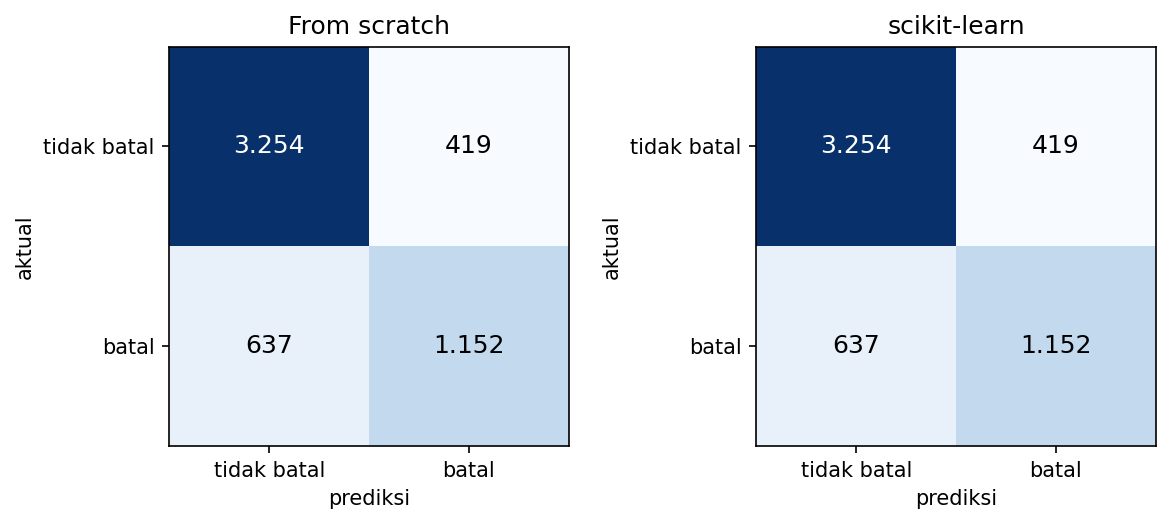
\includegraphics[width=0.8\textwidth]{lr/lr_confusion_matrix.png}
	\caption{\textit{Confusion matrix} LR tanpa penalti (konfigurasi terbaik) pada \texttt{val\_set}, \textit{from scratch} (kiri) dan \textit{scikit-learn} (kanan)}
	\label{fig:lr-cm}
\end{figure}

\subsubsection{Kurva \textit{Loss}}
Gambar~\ref{fig:lr-loss} memperlihatkan nilai fungsi tujuan $J$ (\textit{log-loss} ditambah penalti) pada \texttt{train\_set} untuk setiap penalti, dengan kedua \textit{solver} yang diimplementasikan. Nilai $J$ tidak dapat dibandingkan langsung antarpenalti karena suku penaltinya berbeda; yang dibandingkan adalah bentuk konvergensinya.

\begin{figure}[H]
	\centering
	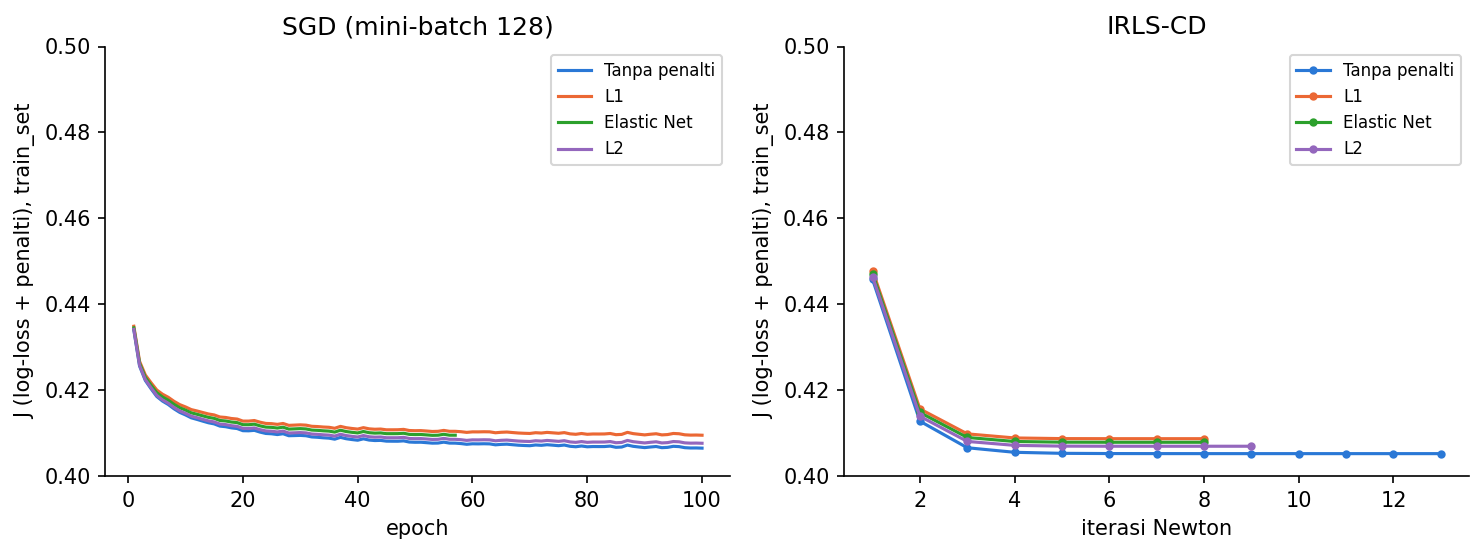
\includegraphics[width=\textwidth]{lr/lr_loss_curves.png}
	\caption{Kurva $J$ per iterasi pada \texttt{train\_set}: SGD \textit{mini-batch} per \textit{epoch} (kiri) dan IRLS-CD per iterasi Newton (kanan)}
	\label{fig:lr-loss}
\end{figure}

\begin{itemize}
	\item \textbf{SGD} menurun cepat pada sekitar 10 \textit{epoch} pertama, lalu melandai dan masih turun perlahan saat berhenti. Tiga dari empat konfigurasi berhenti di batas 100 \textit{epoch}; hanya \textit{Elastic Net} berhenti lebih awal (57 \textit{epoch}) karena perubahan \textit{loss} di bawah toleransi. Kurvanya sedikit bergerigi karena gradien \textit{mini-batch} bersifat acak, dan \textit{learning rate} yang tetap membuatnya tidak pernah menetap di satu titik. Ini berarti SGD belum benar-benar konvergen pada 100 \textit{epoch}.
	\item \textbf{IRLS-CD} mencapai nilai akhirnya dalam 8 sampai 13 iterasi. Pada tanpa penalti dibutuhkan 13 iterasi, lebih banyak daripada penalti lain (8 sampai 9), karena tidak ada suku penalti yang membuat masalah lebih terkondisi dengan baik; model ini juga memiliki kolom yang kolinear (Subbab~\ref{subsec:lr-implementasi}).
	\item Untuk setiap penalti, $J$ akhir IRLS-CD lebih rendah daripada SGD: 0,4052 terhadap 0,4065 (tanpa penalti), 0,4087 terhadap 0,4095 (L1), 0,4079 terhadap 0,4095 (\textit{Elastic Net}), dan 0,4070 terhadap 0,4076 (L2). Karena fungsi tujuannya konveks, selisih ini adalah jarak SGD ke optimum, yang menjelaskan mengapa IRLS-CD sedikit lebih baik pada validasi (Subbab~\ref{subsubsec:lr-optimasi}).
\end{itemize}

\subsubsection{Analisis}
\paragraph{Hasil praktis identik.} Untuk keempat penalti, selisih Macro F1 antara \textit{scratch} dan \textit{scikit-learn} paling besar 0,0003 (L1), ROC-AUC berselisih paling besar $10^{-4}$, dan matriks konfusinya sama persis atau berbeda satu baris. Label prediksi sama pada 99,98\% sampai 100\% baris, dan korelasi peluang model terbaik 1,0000. Ini sesuai harapan: keduanya meminimumkan fungsi tujuan konveks yang sama, sehingga IRLS-CD dan \textit{solver} \textit{scikit-learn} menuju optimum yang sama. Perbedaan kecil pada L1 berasal dari kriteria berhenti yang berbeda: \texttt{saga} berhenti pada toleransi tertentu dan belum tentu tepat di optimum, sedangkan IRLS-CD pada L1 menghasilkan nilai $J$ sedikit lebih rendah (0,408706 terhadap 0,408709).

\paragraph{Bobot dan \textit{sparsity}.} Selisih bobot terbesar (nilai mutlak) antara kedua implementasi adalah 5,85 (tanpa penalti), 0,100 (L1), 0,062 (\textit{Elastic Net}), dan 0,0028 (L2). Selisih besar pada model tanpa penalti bukan tanda kesalahan. Kolom \textit{one-hot} setiap fitur kategorikal bersama bias saling kolinear (matriks fitur ditambah bias hanya berperingkat 92 dari 101), sehingga bobotnya tidak unik walaupun prediksinya identik (label sama 100\%). Penalti L2 memperbaiki hal ini karena menjamin solusi yang unik, dan itu terlihat dari selisih bobotnya yang sangat kecil. Pada L1 dan \textit{Elastic Net}, kedua implementasi menghasilkan bobot tepat nol dalam jumlah hampir sama (16 terhadap 14 dan 13 terhadap 12). Selisih satu sampai dua bobot muncul karena bobot-bobot itu berada tepat di dekat ambang \textit{soft-thresholding}, dan kriteria berhenti kedua \textit{solver} berbeda.

\paragraph{Waktu pelatihan.} Waktu pada Tabel~\ref{tab:lr-hasil} hanya perkiraan kasar karena diukur sekali pada komputer yang sedang dipakai untuk pekerjaan lain. Pengulangan pengukuran yang sama memberi angka yang berbeda beberapa kali lipat (misalnya \textit{scikit-learn} tanpa penalti: 10,9 detik pada satu kali jalan dan 35,8 detik pada kali lain), sehingga hanya selisih yang besar yang bermakna. Terlihat dua pola. \textit{Scikit-learn} jauh lebih cepat pada L2 (2,2 terhadap 13,1 detik), karena \texttt{lbfgs} yang ditulis dalam kode teroptimasi hanya perlu menghitung gradien, sedangkan IRLS-CD membentuk dan memperbarui matriks Gram $101 \times 101$ pada setiap iterasi. Sebaliknya \textit{scratch} jauh lebih cepat pada L1 dan \textit{Elastic Net} (sekitar 9 sampai 11 detik terhadap lebih dari 360 detik), karena \texttt{saga} adalah metode orde pertama yang butuh banyak lintasan data sampai mencapai toleransi $10^{-6}$ pada fitur yang berkorelasi, sedangkan IRLS-CD memakai informasi orde kedua dan konvergen dalam kurang dari sepuluh iterasi. Pada model tanpa penalti \textit{scratch} juga lebih cepat (7,5 terhadap 35,8 detik), tetapi selisih ini paling tidak stabil antarpengukuran. Perbandingan ini adil hanya dalam arti kedua \textit{solver} diminta ketat pada toleransi masing-masing; \textit{scikit-learn} dapat dipercepat dengan toleransi yang lebih longgar tanpa mengubah hasil prediksi secara berarti.

\paragraph{Keterbatasan.} (i) Perbandingan dilakukan pada satu pembagian \texttt{train\_set}/\allowbreak\texttt{val\_set}, dan \texttt{val\_set} ikut dipakai dalam CV sehingga bukan estimasi independen (Subbab~\ref{subsec:lr-validasi}). (ii) Selisih antarpenalti (paling besar 0,002 pada Macro F1) jauh di bawah simpangan baku antar-\textit{fold} (0,0073), sehingga urutan penalti pada tabel tidak bermakna secara statistik. (iii) Seluruh hasil \textit{scratch} di atas memakai IRLS-CD. Hasil \textit{scratch} dengan \textit{solver} SGD yang sesuai materi kelas sedikit di bawahnya (Subbab~\ref{subsubsec:lr-optimasi}); karena SGD belum konvergen, selisihnya dengan \textit{scikit-learn} akan lebih besar dari angka di atas.

\subsection{Bonus LR}
\label{subsec:lr-bonus}

\todo{Hapus subbab bonus yang tidak dikerjakan.}

\subsubsection{Video Kontur \textit{Log-Loss}}
\todo{Video kontur \textit{log-loss} pada bidang $(\theta_0, \theta_1)$ beserta lintasan parameter selama pelatihan. Jelaskan cara pembuatannya, cantumkan cuplikan \textit{frame}, dan tautan atau lokasi berkas video.}

\begin{figure}[H]
	\centering
	\placeholdergambar{Video Kontur \textit{Log-Loss}}
	\caption{Video Kontur \textit{Log-Loss} LR}
	\label{fig:lr-bonus-0}
\end{figure}

\subsubsection{Algoritma Optimasi di Luar Materi Kelas}
\todo{Jika ada: jelaskan algoritmanya, mengapa dapat mengoptimasi model, bukti perbaikannya (sebelum vs sesudah), dan \textbf{referensinya (tanpa referensi bonus dianulir)}. Misalnya \textit{mini-batch} SGD dengan \textit{early stopping}, \textit{momentum}, Adam, atau \textit{proximal gradient} untuk L1.}


\section{\textit{Support Vector Machine} (SVM)}
\label{sec:svm}

\textit{Support Vector Machine} (SVM) mencari \textit{hyperplane} pemisah dua kelas dengan margin terbesar, dan lewat \textit{kernel trick} dapat membentuk batas keputusan yang nonlinear tanpa membangun fitur nonlinear secara eksplisit \cite{ruskanda-svm-what,ruskanda-svm-linear,ruskanda-svm-nonlinear}. Model ini cocok untuk data pembatalan pesanan karena batas antara pesanan yang batal dan yang tidak batal tidak linear terhadap fitur (kernel Laplacian jauh mengungguli kernel linear, Subbab~\ref{subsec:svm-validasi}), jumlah barisnya (27.309) masih terjangkau oleh pelatihan berbasis kernel, dan model hanya ditentukan oleh \textit{support vector}, yaitu titik di sekitar dan di dalam margin. Konsekuensinya, SVM sensitif terhadap skala fitur dan tidak menerima nilai kosong, sehingga \textit{preprocessing} menentukan hasilnya (Subbab~\ref{subsec:svm-preprocessing}).

Implementasi \textit{from scratch} berada pada kelas \texttt{SVM} di \nolinkurl{src/algoritma/svm/svm.py} dan hanya memakai NumPy. Kelas ini mendukung kernel \textit{linear}, \textit{polynomial}, dan \textit{Gaussian} (RBF) yang diwajibkan, ditambah kernel Laplacian. Masalah dual diselesaikan dengan \textit{Sequential Minimal Optimization} (SMO) \cite{platt1998smo}, dengan pemilihan pasangan variabel berdasarkan informasi orde kedua \cite{fan2005wss} dan \textit{cache} baris kernel seperti pada LIBSVM \cite{chang2011libsvm}. Tiga kernel wajib divalidasi terhadap \texttt{sklearn.svm.SVC} \cite{pedregosa2011sklearn} dan hasilnya setara (Subbab~\ref{subsec:svm-hasil}).

Fokus bab ini adalah model terbaik, yaitu SVM dengan kernel Laplacian $K(a, b) = \exp(-\lVert W(a-b)\rVert_1 / 20)$, $C = 2$, dan 46 fitur yang distandardisasi lalu dikalikan bobot fitur $W$ yang dipelajari dari data latih. Fitur tersebut mencakup fitur ``saudara'', yaitu rata-rata label pesanan lain yang kemungkinan satu rombongan (Subbab~\ref{subsec:svm-preprocessing}). Dengan \textit{stratified} 5-\textit{fold cross validation} pada seluruh data latih bersih, model ini mencapai Macro F1 \textit{out-of-fold} 0,8703 (rata-rata 7 \textit{seed}, simpangan baku antar-\textit{seed} 0,0007) dan 0,8699 pada empat \textit{seed} konfirmasi yang tidak dipakai memilih konfigurasi. Skor publik Kaggle model yang dilatih pada seluruh data latih adalah 0,87464 (Bagian~\ref{sec:kaggle}). Sebagai pembanding, kernel wajib terbaik pada protokol notebook (hold-out 20\%, 6.000 baris latih) hanya mencapai Macro F1 0,8251, sedangkan kernel Laplacian dengan bobot fitur mencapai 0,8561 pada protokol yang sama. Keunggulan ini muncul dari tiga hal yang dibahas bertahap pada subbab berikut: jarak L1 pada kernel, bobot fitur, dan fitur saudara. Selisih SVM terhadap pohon keputusan C4.5 dengan 46 fitur yang sama (0,8685) kecil dan selang kepercayaannya masih mencakup nol (Subbab~\ref{subsec:svm-validasi}).

\subsection{Implementasi \textit{From Scratch}}
\label{subsec:svm-implementasi}

\subsubsection{Landasan Teori}

\paragraph{\textit{Hyperplane} dan margin.} Misalkan data latih $\{(x_i, y_i)\}_{i=1}^{n}$ dengan $x_i \in \mathbb{R}^d$ dan label $y_i \in \{-1, +1\}$. Pada implementasi, kelas batal diberi label $+1$ dan kelas tidak batal $-1$. SVM mencari \textit{hyperplane} $w \cdot x + b = 0$ yang memisahkan kedua kelas. Jarak titik $x$ ke \textit{hyperplane} adalah $|w \cdot x + b| / \lVert w\rVert$. Jika titik terdekat dari kedua kelas dinormalkan sehingga memenuhi $y_i(w \cdot x_i + b) = 1$, lebar margin antara kedua kelas adalah $2 / \lVert w\rVert$, sehingga memaksimumkan margin sama dengan meminimumkan $\lVert w\rVert$ \cite{ruskanda-svm-what,ruskanda-svm-linear}. Titik yang berada tepat di batas margin disebut \textit{support vector}.

\paragraph{\textit{Soft margin} dan parameter $C$.} Data nyata tidak dapat dipisahkan sempurna, sehingga setiap titik diberi variabel kendur (\textit{slack}) $\xi_i \ge 0$ yang mengukur seberapa jauh titik itu melanggar margin \cite{ruskanda-svm-nonlinear}. Masalah primalnya adalah
\begin{equation}
	\min_{w,\,b,\,\xi}\ \tfrac{1}{2}\lVert w\rVert^2 + \sum_{i=1}^{n} C_i\,\xi_i
	\quad \text{dengan} \quad y_i\big(w \cdot \varphi(x_i) + b\big) \ge 1 - \xi_i,\ \ \xi_i \ge 0,
	\label{eq:svm-primal}
\end{equation}
dengan $\varphi$ pemetaan fitur ke ruang berdimensi lebih tinggi (dipakai secara implisit lewat kernel). Pada implementasi $C_i = C$ untuk semua titik, kecuali jika \texttt{class\_weight} diberikan: $C_i = C \cdot c_{y_i}$ dengan $c_{y_i}$ bobot kelas titik tersebut (dipakai pada bonus \textit{cost-sensitive}, Subbab~\ref{subsubsec:svm-cost}). $C$ besar menghukum pelanggaran margin dengan keras sehingga margin menyempit dan model cenderung \textit{overfit}; $C$ kecil membiarkan lebih banyak pelanggaran sehingga margin lebar dan model cenderung \textit{underfit}. Pengaruh ini terlihat langsung pada hasil \textit{tuning} (Subbab~\ref{subsec:svm-validasi}).

\paragraph{Lagrangian dan bentuk dual.} Dengan pengali Lagrange $\alpha_i \ge 0$ untuk kendala margin dan $\mu_i \ge 0$ untuk $\xi_i \ge 0$,
\begin{equation}
	\mathcal{L}(w, b, \xi, \alpha, \mu) = \tfrac{1}{2}\lVert w\rVert^2 + \sum_i C_i\xi_i - \sum_i \alpha_i\big[y_i(w \cdot \varphi(x_i) + b) - 1 + \xi_i\big] - \sum_i \mu_i\xi_i .
	\label{eq:svm-lagrangian}
\end{equation}
Menurunkan $\mathcal{L}$ terhadap variabel primal dan menyamakannya dengan nol memberi
\begin{align}
	\frac{\partial \mathcal{L}}{\partial w} = 0 &\Rightarrow w = \sum_i \alpha_i y_i\,\varphi(x_i), \\
	\frac{\partial \mathcal{L}}{\partial b} = 0 &\Rightarrow \sum_i \alpha_i y_i = 0, \\
	\frac{\partial \mathcal{L}}{\partial \xi_i} = 0 &\Rightarrow \alpha_i = C_i - \mu_i .
\end{align}
Karena $\mu_i \ge 0$, diperoleh kotak batas $0 \le \alpha_i \le C_i$. Substitusi ke $\mathcal{L}$ menghilangkan $w$, $b$, dan $\xi$, sehingga tersisa masalah dual yang hanya bergantung pada $\alpha$ dan hasil kali dalam $K(x_i, x_j) = \varphi(x_i)\cdot\varphi(x_j)$:
\begin{equation}
	\max_{\alpha}\ \sum_{i} \alpha_i - \tfrac{1}{2}\sum_{i}\sum_{j} \alpha_i\alpha_j\,y_i y_j\,K(x_i, x_j)
	\quad \text{dengan} \quad 0 \le \alpha_i \le C_i,\ \ \sum_i \alpha_i y_i = 0 .
	\label{eq:svm-dual}
\end{equation}
Fungsi keputusan model hanya melibatkan titik dengan $\alpha_i > 0$ (\textit{support vector}):
\begin{equation}
	f(x) = \sum_{i} \alpha_i y_i\,K(x_i, x) + b, \qquad \hat{y} = \begin{cases} +1 & f(x) > t \\ -1 & \text{lainnya,} \end{cases}
	\label{eq:svm-decision}
\end{equation}
dengan $t$ ambang keputusan (\texttt{threshold} pada \texttt{predict}, bawaan 0). Nilai $f(x)$ juga disebut skor keputusan, dan $|f(x)|/\lVert w\rVert$ adalah jarak $x$ ke \textit{hyperplane} di ruang fitur kernel.

\paragraph{Kondisi KKT.} Solusi optimum memenuhi kondisi \textit{Karush-Kuhn-Tucker} berikut, yang menjadi dasar kriteria berhenti SMO:
\begin{equation}
	\alpha_i = 0 \Rightarrow y_i f(x_i) \ge 1, \qquad
	0 < \alpha_i < C_i \Rightarrow y_i f(x_i) = 1, \qquad
	\alpha_i = C_i \Rightarrow y_i f(x_i) \le 1 .
	\label{eq:svm-kkt}
\end{equation}
Titik dengan $\alpha_i = 0$ berada di luar margin dan tidak memengaruhi model. Titik dengan $0 < \alpha_i < C_i$ (\textit{free support vector}) tepat di batas margin. Titik dengan $\alpha_i = C_i$ berada di dalam margin atau salah sisi.

\paragraph{\textit{Kernel trick} dan empat kernel.} Persamaan \eqref{eq:svm-dual} dan \eqref{eq:svm-decision} hanya memakai $K(a, b) = \varphi(a)\cdot\varphi(b)$, sehingga $\varphi$ tidak pernah dihitung. Cukup mengganti $K$ untuk mendapatkan batas keputusan nonlinear \cite{ruskanda-svm-nonlinear}. Tabel~\ref{tab:svm-kernel} merangkum empat kernel yang diimplementasikan. Kernel \textit{sigmoid} pada materi kelas tidak diimplementasikan karena spesifikasi hanya mewajibkan tiga kernel pertama.

\begin{table}[H]
	\centering
	\caption{Kernel yang diimplementasikan pada \texttt{SVM}}
	\label{tab:svm-kernel}
	\small
	\begin{tabularx}{\textwidth}{l l Y}
		\toprule
		\textbf{\texttt{kernel}} & $K(a, b)$ & \textbf{Parameter dan catatan} \\
		\midrule
		\texttt{"linear"} & $a \cdot b$ & Tanpa parameter. Koefisien $w = \sum_i \alpha_i y_i x_i$ tersedia pada atribut \texttt{coef\_}. \\
		\texttt{"poly"} & $(\gamma\,a \cdot b + r)^{p}$ & $\gamma$ (\texttt{gamma}), $r$ (\texttt{coef0}), derajat $p$ (\texttt{degree}). \\
		\texttt{"rbf"} (\textit{Gaussian}) & $\exp\!\big(-\gamma\lVert a - b\rVert_2^2\big)$ & $\gamma$ (\texttt{gamma}). Jarak L2 kuadrat. \\
		\texttt{"laplacian"} & $\exp\!\big(-\gamma\lVert a - b\rVert_1\big)$ & $\gamma$ (\texttt{gamma}). Jarak L1 (jumlah selisih mutlak per fitur). \\
		\bottomrule
	\end{tabularx}
\end{table}

Nilai \texttt{gamma="scale"} (bawaan) berarti $\gamma = 1/(d \cdot \operatorname{Var}(X))$ dengan $\operatorname{Var}(X)$ variansi seluruh elemen matriks latih, dan \texttt{gamma="auto"} berarti $\gamma = 1/d$, sama seperti pada \textit{scikit-learn} \cite{pedregosa2011sklearn}. Pada data yang sudah distandardisasi, $\operatorname{Var}(X) \approx 1$ sehingga \texttt{"scale"} kira-kira $1/d$. Kernel \textit{Gaussian} dan Laplacian memenuhi $K(a, a) = 1$, sedangkan kernel \textit{linear} dan \textit{polynomial} tidak. Karena itu implementasi menghitung diagonal kernel secara terpisah (\texttt{\_gram\_diagonal} pada Tabel~\ref{tab:svm-fungsi}), tanpa membentuk seluruh matriks.

\paragraph{Kernel Laplacian dan alasan jarak L1.} Kernel Laplacian termasuk keluarga kernel $\exp(-\rho\sum_k |a_k - b_k|^{\beta})$ yang dipakai untuk klasifikasi histogram citra oleh \cite{chapelle1999histogram}, dengan $\beta = 1$. Perbedaannya dengan \textit{Gaussian} hanya pada jarak: Gaussian memakai jumlah kuadrat selisih, Laplacian memakai jumlah selisih mutlak. Pada data ini ada dua alasan jarak L1 lebih sesuai. Pertama, jarak L2 kuadrat memperbesar selisih ekstrem secara kuadratik. Setelah standardisasi, satu penanda kosong dengan prevalensi 4,0\% (\texttt{missing\_needs\_parking}) bernilai 4,88 simpangan baku saat bernilai 1, sehingga ketidakcocokannya menyumbang 23,8 pada jarak L2 kuadrat tetapi 4,88 pada jarak L1. Nilai ekstrem juga ada pada fitur numerik: nilai maksimum \texttt{prior\_completed\_bookings} berada 36 simpangan baku dari rata-rata dan \texttt{num\_children} 24,9 simpangan baku (data pengembangan). Pada L2 kuadrat sumbangan keduanya masing-masing sekitar 1.300 dan 620, pada L1 hanya 36 dan 25. Kedua, jarak L1 menjumlahkan sumbangan tiap fitur tanpa saling memperkuat, sehingga pembobotan per fitur (Subbab~\ref{subsubsec:svm-agop-teori}) bekerja langsung sebagai skala tiap sumbu. Kedua alasan ini adalah penjelasan yang masuk akal, bukan bukti. Buktinya adalah hasil empiris pada Subbab~\ref{subsec:svm-validasi} dan \ref{subsec:svm-hasil}. Karena bentuk eksponensial dari jarak L1 adalah kernel positif semidefinit, masalah dual \eqref{eq:svm-dual} tetap konkaf dan SMO konvergen. Implementasi \texttt{"laplacian"} tidak dapat memakai trik $\lVert a-b\rVert^2 = \lVert a\rVert^2 + \lVert b\rVert^2 - 2a\cdot b$ (perkalian matriks) seperti \textit{Gaussian}, sehingga jaraknya dihitung per kolom fitur (Kode~\ref{lst:svm-l1}) dan lebih lambat per baris kernel.

\subsubsection{Algoritma SMO}
Masalah dual \eqref{eq:svm-dual} adalah \textit{quadratic programming} dengan $n$ variabel, satu kendala persamaan, dan kendala kotak. \textit{Sequential Minimal Optimization} (SMO) \cite{platt1998smo} menyelesaikannya dengan mengubah dua variabel $\alpha_i, \alpha_j$ pada setiap langkah. Dua adalah jumlah paling sedikit yang memungkinkan kendala $\sum_k \alpha_k y_k = 0$ tetap terpenuhi, dan masalah dua variabel memiliki solusi tertutup, sehingga tidak diperlukan \textit{solver} QP. Implementasi mengikuti bentuk SMO pada LIBSVM \cite{chang2011libsvm} dengan pemilihan pasangan orde kedua \cite{fan2005wss}. Notasinya sebagai berikut.

\paragraph{Skor.} Untuk setiap titik $t$ didefinisikan
\begin{equation}
	s_t = y_t - \sum_{k}\alpha_k y_k K(x_k, x_t) = y_t - \big(f(x_t) - b\big),
	\label{eq:svm-score}
\end{equation}
yang pada kode adalah larik \texttt{score}. Pada awal pelatihan $\alpha = 0$ sehingga $s = y$. Gradien fungsi tujuan dual terhadap $\alpha_t$ sama dengan $y_t s_t$, sehingga $s_t$ cukup untuk memantau optimalitas. Selama pelatihan hanya vektor $s$, vektor $\alpha$, dan baris kernel yang sedang dipakai yang disimpan, bukan seluruh matriks kernel.

\paragraph{Himpunan indeks dan kondisi optimalitas.} Titik yang $\alpha$-nya masih boleh naik atau turun dikelompokkan menurut arah geraknya terhadap kendala $\sum\alpha_k y_k = 0$:
\begin{align}
	I_{\text{naik}} &= \{t : (y_t = +1,\ \alpha_t < C_t) \lor (y_t = -1,\ \alpha_t > 0)\}, \nonumber\\
	I_{\text{turun}} &= \{t : (y_t = +1,\ \alpha_t > 0) \lor (y_t = -1,\ \alpha_t < C_t)\},
	\label{eq:svm-indeks}
\end{align}
yang pada kode adalah \texttt{can\_rise} dan \texttt{can\_fall}. Menerapkan Persamaan~\eqref{eq:svm-kkt} pada $s_t = y_t - f(x_t) + b$ menunjukkan bahwa solusi optimum ada jika dan hanya jika terdapat $b$ dengan $s_t \le b$ untuk $t \in I_{\text{naik}}$ dan $s_t \ge b$ untuk $t \in I_{\text{turun}}$. Titik \textit{free support vector} memenuhi keduanya sehingga $s_t = b$. Dengan demikian optimalitas setara dengan
\begin{equation}
	m(\alpha) - M(\alpha) \le 0, \qquad m(\alpha) = \max_{t \in I_{\text{naik}}} s_t, \quad M(\alpha) = \min_{t \in I_{\text{turun}}} s_t .
\end{equation}
Pada praktiknya pelatihan berhenti jika $m(\alpha) - M(\alpha) < \tau$ dengan $\tau$ = \texttt{tol} (bawaan $10^{-3}$, sama dengan \textit{scikit-learn}), atau jika \texttt{n\_iter\_} mencapai \texttt{max\_iter}. Pada kasus kedua, \texttt{fit} mengeluarkan peringatan dan tetap mengembalikan model yang dapat dipakai.

\paragraph{Pemilihan pasangan orde kedua.} Titik pertama dipilih sebagai pelanggar terbesar, $i = \arg\max_{t \in I_{\text{naik}}} s_t$. Titik kedua dipilih dari $I_{\text{turun}}$ dengan menimbang kenaikan fungsi tujuan yang sebenarnya, bukan hanya selisih skor. Jika $\alpha_i y_i$ naik sebesar $\delta$ dan $\alpha_j y_j$ turun sebesar $\delta$ (kendala persamaan tetap terjaga), fungsi tujuan dual berubah menurut
\begin{equation}
	\Delta D(\delta) = \delta\,(s_i - s_j) - \tfrac{1}{2}\,a_{ij}\,\delta^2, \qquad a_{ij} = K_{ii} + K_{jj} - 2K_{ij},
\end{equation}
dengan $a_{ij} \ge 0$ kelengkungan di sepanjang arah tersebut. Parabola ini mencapai puncak di $\delta^{*} = (s_i - s_j)/a_{ij}$ dengan kenaikan $(s_i - s_j)^2 / (2a_{ij})$. Karena itu
\begin{equation}
	g_t = s_i - s_t, \qquad a_{it} = \max\big(K_{ii} + K_{tt} - 2K_{it},\ \tau_a\big), \qquad
	j = \arg\max_{t \in I_{\text{turun}},\ g_t > 0}\ \frac{g_t^{2}}{a_{it}},
	\label{eq:svm-pasangan}
\end{equation}
dengan $\tau_a = 10^{-12}$ (konstanta \texttt{TAU}, mengikuti LIBSVM) agar tidak terjadi pembagian dengan nol bila kelengkungan nol atau sedikit negatif akibat pembulatan. Bandingkan dengan pemilihan orde pertama yang hanya mengambil $t$ dengan $s_t$ terkecil: pasangan itu memiliki selisih skor terbesar, tetapi bisa memiliki kelengkungan besar sehingga langkahnya pendek dan kenaikan tujuannya kecil.

\paragraph{Langkah dan pemotongan ke kotak.} Langkah tanpa kendala adalah $\delta^{*}$. Langkah tersebut dipotong oleh sisa ruang di dalam kotak $[0, C_t]$ untuk kedua variabel:
\begin{equation}
	r_i = \begin{cases} C_i - \alpha_i & y_i = +1 \\ \alpha_i & y_i = -1 \end{cases}, \qquad
	r_j = \begin{cases} \alpha_j & y_j = +1 \\ C_j - \alpha_j & y_j = -1 \end{cases}, \qquad
	\delta = \min\{\delta^{*},\ r_i,\ r_j\},
\end{equation}
dan pembaruannya
\begin{equation}
	\alpha_i \leftarrow \alpha_i + y_i\,\delta, \qquad \alpha_j \leftarrow \alpha_j - y_j\,\delta, \qquad
	s_t \leftarrow s_t - \delta\,\big(K_{it} - K_{jt}\big)\quad \forall t .
	\label{eq:svm-update}
\end{equation}
Karena $y_i \cdot y_i\delta + y_j\cdot(-y_j\delta) = 0$, kendala $\sum\alpha_k y_k = 0$ tidak pernah dilanggar. Pembaruan skor muncul dari Persamaan~\eqref{eq:svm-score}: perubahan $\alpha_i y_i$ sebesar $+\delta$ dan $\alpha_j y_j$ sebesar $-\delta$ mengubah $f(x_t) - b$ sebesar $\delta(K_{it} - K_{jt})$. Jika langkah terpotong oleh batas (\texttt{step == room}), variabel yang bersangkutan langsung diset tepat ke $0$ atau $C_t$ oleh fungsi \texttt{\_move}, bukan hasil penjumlahan, agar galat pembulatan tidak membuat $\alpha$ berada sedikit di dalam atau di luar kotak. Setelah itu keanggotaan $i$ dan $j$ pada $I_{\text{naik}}$ dan $I_{\text{turun}}$ diperbarui.

\paragraph{Bias.} Titik \textit{free support vector} memenuhi $s_t = b$, sehingga
\begin{equation}
	b = \frac{1}{|F|}\sum_{t \in F} s_t, \qquad F = \{t : 0 < \alpha_t < C_t\},
\end{equation}
mengikuti LIBSVM \cite{chang2011libsvm}. Jika tidak ada \textit{free support vector}, bias diambil dari titik tengah $(m + M)/2$.

\subsubsection{Bobot Fitur dengan AGOP}
\label{subsubsec:svm-agop-teori}
Kernel Laplacian pada model terbaik tidak memakai fitur standar secara langsung, melainkan $K(a, b) = \exp\big(-\sum_k w_k|a_k - b_k| / L\big)$ dengan $L = 20$ (jadi $\gamma = 1/L = 0{,}05$) dan bobot $w_k \ge 0$ per fitur. Memakai bobot ini setara dengan mengalikan setiap kolom fitur dengan $w_k$ sebelum dimasukkan ke \texttt{SVM}, dan itulah yang dilakukan kode (\texttt{A * w}). Bobot dipelajari dari data latih dengan prosedur yang diadaptasi dari \textit{Average Gradient Outer Product} (AGOP) pada \textit{Recursive Feature Machine} \cite{radhakrishnan2024rfm}. Versi di sini disederhanakan: hanya diagonal AGOP yang dipakai, jaraknya L1, dan bobot adalah akar dari RMS gradien. Prosedur ini bukan replikasi penuh makalah tersebut. Satu putaran terdiri atas langkah berikut, dengan $X$ fitur terstandardisasi ($n \times d$) dan target $t_i = y_i - \tfrac12 \in \{\pm\tfrac12\}$. Pada putaran pertama $w = \mathbf{1}$, dan putaran dilakukan dua kali (\texttt{ROUNDS = 2}).

\begin{enumerate}
	\item \textbf{Model pengganti.} Dipilih $m = 1.500$ pusat acak $z_c$ dari baris latih (\texttt{CENTRES}), dan dipasang model $f(x) = \sum_{c=1}^{m} \beta_c\,K_w(x, z_c)$ dengan $K_w$ kernel Laplacian berbobot $w$ saat ini. Model ini adalah \textit{kernel ridge regression} \cite{saunders1998ridge} yang disederhanakan dengan pendekatan Nystr\"om \cite{williams2001nystrom}, yaitu pusat dibatasi pada himpunan bagian $m \ll n$ baris:
	\begin{equation}
		\min_{\beta}\ \sum_{i=1}^{n}\big(f(x_i) - t_i\big)^2 + \lambda\,\beta^{\top}K_{ZZ}\beta
		\ \Longrightarrow\
		\big(K_{XZ}^{\top}K_{XZ} + \lambda K_{ZZ} + \epsilon I\big)\beta = K_{XZ}^{\top}t,
		\label{eq:svm-nystrom}
	\end{equation}
	dengan $\lambda = 0{,}3$ (\texttt{RIDGE}) dan $\epsilon = 10^{-6}$ kali rata-rata diagonal matriks sistem (penstabil numerik). $K_{XZ}^{\top}K_{XZ}$ dijumlahkan per blok 2.000 baris agar memori tidak bergantung pada $n$.
	\item \textbf{Gradien.} Turunan model terhadap fitur ke-$k$ pada titik $x$ (turunan $|u|$ adalah $\operatorname{sign}(u)$, terdefinisi hampir di mana-mana) adalah
	\begin{equation}
		\frac{\partial f}{\partial x_k}(x) = -\frac{w_k}{L}\sum_{c=1}^{m}\beta_c\,K_w(x, z_c)\,\operatorname{sign}\big(x_k - z_{ck}\big).
		\label{eq:svm-gradien}
	\end{equation}
	Gradien dihitung pada $q = 4.000$ baris acak (\texttt{GRADIENT\_ROWS}). Pada kode, jumlahnya dihitung pada koordinat yang sudah berbobot, lalu dikalikan $w_k$ sesuai aturan rantai.
	\item \textbf{Diagonal AGOP dan bobot baru.} Rata-rata kuadrat gradien per fitur adalah diagonal AGOP,
	\begin{equation}
		G_k = \frac{1}{q}\sum_{r=1}^{q}\Big(\frac{\partial f}{\partial x_k}(x_r)\Big)^{2}, \qquad
		w_k^{\text{baru}} \propto \sqrt{\sqrt{G_k}} = G_k^{1/4}, \qquad \sum_{k=1}^{d} \big(w_k^{\text{baru}}\big)^2 = d .
		\label{eq:svm-bobot}
	\end{equation}
	Fitur yang membuat prediksi model pengganti berubah banyak ketika digeser mendapat bobot besar. Pangkat $1/4$ pada $G_k$ (akar dari RMS gradien) dipilih lewat validasi silang (pangkat 0,35 dan 0,7 pada RMS lebih rendah, Tabel~\ref{tab:svm-ablasi}). Normalisasi $\sum_k w_k^2 = d$ menjaga rata-rata kuadrat bobot tetap 1, sehingga skala jarak keseluruhan tidak berubah dan $L = 20$ tetap bermakna. Bobot akhir dibulatkan ke tiga desimal.
\end{enumerate}

Bobot ini bekerja sebagai pemilihan fitur yang halus: fitur tidak relevan tidak dibuang tetapi diperkecil pengaruhnya pada jarak (Tabel~\ref{tab:svm-bobot}). Prosedur ini jauh lebih mahal daripada standardisasi. Pada $n = 27.309$, $m = 1.500$, dan $d = 46$, pembentukan $K_{XZ}^{\top}K_{XZ}$ membutuhkan sekitar $n m^2 \approx 6{,}1 \times 10^{10}$ operasi kali-tambah (BLAS), jarak L1 antara seluruh baris dan pusat membutuhkan $n m d \approx 1{,}9 \times 10^{9}$ operasi, dan penyelesaian sistem $m \times m$ sekitar $m^3 \approx 3{,}4 \times 10^{9}$ operasi, semuanya per putaran. Bobot dihitung ulang dari awal untuk setiap pembagian data, sehingga tidak bocor dari data validasi (Subbab~\ref{subsec:svm-preprocessing}).

\subsubsection{Struktur Kelas dan Fungsi}
Kelas \texttt{SVM} berada pada \nolinkurl{src/algoritma/svm/svm.py} dan hanya memakai NumPy. Fitur dibangun oleh fungsi pada \nolinkurl{src/kaggle/booking_features.py} (pandas dan NumPy). Tabel~\ref{tab:svm-fungsi} merangkum fungsi dan metode pada \texttt{svm.py}, dan Tabel~\ref{tab:svm-fitur-fungsi} merangkum fungsi pada \texttt{booking\_features.py}.

\begin{table}[H]
	\centering
	\caption{Deskripsi kelas dan fungsi SVM (\texttt{src/algoritma/svm/svm.py})}
	\label{tab:svm-fungsi}
	\small
	\begin{tabularx}{\textwidth}{l Y}
		\toprule
		\textbf{Fungsi/Metode} & \textbf{Deskripsi} \\
		\midrule
		\texttt{KERNELS}, \texttt{TAU} & Tuple nama kernel yang sah (\texttt{linear}, \texttt{poly}, \texttt{rbf}, \texttt{laplacian}) dan batas bawah kelengkungan $\tau_a = 10^{-12}$. \\
		\texttt{PREDICT\_BATCH\_ROWS}, \texttt{LAPLACIAN\_BATCH\_ROWS} & Jumlah baris data uji yang diproses sekaligus oleh \texttt{decision\_function} (4.096; 256 untuk Laplacian) agar memori matriks kernel terbatas. \\
		\texttt{\_l1\_distances(A, B)} & Matriks jarak L1 antara baris \texttt{A} dan \texttt{B}, dijumlahkan per kolom fitur agar tidak membentuk larik tiga dimensi. Kasus satu baris dihitung langsung. \\
		\texttt{\_KernelRowCache.\_\_init\_\_} & Menyimpan fungsi penghitung baris kernel dan kapasitas \textit{cache} $\max\big(2, \lfloor \texttt{cache\_mb}\cdot 10^6 / (8n)\rfloor\big)$ baris. \\
		\texttt{\_KernelRowCache.\_\_getitem\_\_} & Mengembalikan baris kernel ke-$i$ dari \textit{cache} (kebijakan \textit{least recently used} dengan \texttt{OrderedDict}), atau menghitungnya dan membuang baris terlama jika \textit{cache} penuh. \\
		\texttt{SVM.\_\_init\_\_(...)} & Menyimpan hiperparameter: \texttt{C}, \texttt{kernel}, \texttt{degree}, \texttt{gamma}, \texttt{coef0}, \texttt{tol}, \texttt{max\_iter}, \texttt{class\_weight}, dan \texttt{cache\_mb}. Kernel yang tidak dikenal ditolak dengan \texttt{ValueError}. \\
		\texttt{fit(X, y)} & Memvalidasi masukan (dua kelas, tanpa \texttt{NaN}), memetakan label ke $\pm 1$, menghitung batas kotak $C_i$ dan $\gamma$, memanggil \texttt{\_solve}, lalu menyimpan \texttt{support\_}, \texttt{support\_vectors\_}, \texttt{dual\_coef\_} ($\alpha_i y_i$), \texttt{intercept\_}, dan \texttt{coef\_} (hanya kernel \textit{linear}). \\
		\texttt{decision\_function(X)} & Skor $f(x)$ menurut Persamaan~\eqref{eq:svm-decision}, dihitung per kelompok baris. \\
		\texttt{predict(X, threshold)} & Mengembalikan label kelas positif jika skor lebih besar dari \texttt{threshold} (bawaan 0). Label asli (bukan hanya $\pm 1$) dikembalikan. \\
		\texttt{save(path)} & Menyimpan seluruh objek model dengan \texttt{pickle}. \\
		\texttt{load(path)} & \textit{Class method} yang memuat model dari berkas \textit{pickle}. \\
		\texttt{\_solve(X, sign, upper)} & Inti SMO: memilih pasangan, memperbarui $\alpha$ dan skor, memeriksa kriteria berhenti, dan menghitung bias. Mengembalikan $(\alpha, b)$ dan mengisi \texttt{n\_iter\_}. \\
		\texttt{\_move(value, delta, hits\_bound, upper)} & Memperbarui satu $\alpha$; jika langkah terpotong batas, nilainya diset persis ke $0$ atau \texttt{upper}. \\
		\texttt{\_gram(A, B, B\_squared\_norms)} & Matriks kernel antara baris \texttt{A} dan \texttt{B} untuk kernel yang dipilih. \\
		\texttt{\_gram\_diagonal(squared\_norms)} & Diagonal matriks kernel, $K_{ii}$, tanpa membentuk seluruh matriks. \\
		\texttt{\_resolve\_gamma(X)} & Mengubah \texttt{"scale"} dan \texttt{"auto"} menjadi nilai $\gamma$ numerik. \\
		\texttt{\_box\_limits(y)} & Batas atas $C_i$ tiap titik dari \texttt{class\_weight} (\texttt{None}, \texttt{"balanced"}, atau kamus). \\
		\texttt{\_check\_fitted()} & Melempar \texttt{RuntimeError} jika \texttt{predict} dipanggil sebelum \texttt{fit}. \\
		\texttt{\_as\_matrix(X)} & Mengubah masukan menjadi larik \texttt{float64} \textit{contiguous} dan menolak \texttt{NaN} atau tak hingga. \\
		\bottomrule
	\end{tabularx}
\end{table}

\begin{table}[H]
	\centering
	\caption{Fungsi pembangun fitur dan bobot (\texttt{src/kaggle/booking\_features.py})}
	\label{tab:svm-fitur-fungsi}
	\small
	\begin{tabularx}{\textwidth}{l Y}
		\toprule
		\textbf{Fungsi} & \textbf{Deskripsi} \\
		\midrule
		\texttt{load\_data(data\_dir)} & Membaca \texttt{train.csv} dan \texttt{test.csv} dengan \texttt{id} sebagai teks. \\
		\texttt{clean(train)} & Membuang kolom \texttt{id} lalu baris duplikat (data latih saja). \\
		\texttt{add\_booking\_dates(df)} & Menambahkan \texttt{arr\_ord} (hari sejak 2023-01-01), \texttt{book\_ord} (\texttt{arr\_ord} dikurangi \textit{lead time}), dan \texttt{arr\_dow} (hari dalam minggu). \\
		\texttt{impute\_and\_flag(train, other)} & Imputasi median atau modus yang dipelajari dari data latih, dan penanda \texttt{missing\_*} untuk setiap kolom yang punya nilai kosong di data latih. \\
		\texttt{sibling\_pairs(reference, query, same)} & Mencari saudara tiap baris \texttt{query} pada \texttt{reference} (kunci keras, toleransi, kolom lunak) beserta bobot kedekatan \textit{lead time}. \\
		\texttt{shared\_neighbour\_weights(...)} & Mengalikan bobot pasangan dengan akar indeks Jaccard antar-himpunan saudara. \\
		\texttt{build\_features(train, labels, other, shared\_neighbours)} & Membangun seluruh fitur: tanggal, imputasi, fitur saudara (\texttt{sib\_te}, \texttt{sib\_n}) secara \textit{out-of-fold}, lama menginap, dan \textit{one-hot}. Kolom \texttt{other} disejajarkan dengan kolom data latih. \\
		\texttt{standardize(train, other)} & Transformasi akar, logit, dan $\log(1+x)$ pada tiga kolom, lalu \textit{z-score}; kolom dengan simpangan baku nol dibuang. Mengembalikan nama kolom. \\
		\texttt{laplacian\_gram(A, B, scale)} & Matriks kernel Laplacian $\exp(-\lVert a-b\rVert_1/L)$ untuk penghitungan bobot fitur. \\
		\texttt{feature\_weights(X, y, scale)} & Bobot fitur AGOP diagonal (Persamaan~\eqref{eq:svm-nystrom}--\eqref{eq:svm-bobot}). \\
		\bottomrule
	\end{tabularx}
\end{table}

Konstanta yang dipakai pembangun fitur dan bobot ditunjukkan pada Tabel~\ref{tab:svm-konstanta}.

\begin{table}[H]
	\centering
	\caption{Konstanta pada \texttt{booking\_features.py}}
	\label{tab:svm-konstanta}
	\small
	\begin{tabularx}{\textwidth}{l c Y}
		\toprule
		\textbf{Konstanta} & \textbf{Nilai} & \textbf{Arti} \\
		\midrule
		\texttt{LEAD\_TOLERANCE} & 10 & Selisih \textit{lead time} paling besar antara dua saudara (hari). \\
		\texttt{RATE\_TOLERANCE} & 0,05 & Selisih tarif paling besar, sebagai pecahan dari tarif yang lebih besar. \\
		\texttt{MISSING\_LEAD\_WEIGHT} & 0,1 & Bobot pasangan jika salah satu \textit{lead time} kosong. \\
		\texttt{INNER\_FOLDS} & 5 & Jumlah kelompok acak untuk fitur saudara \textit{out-of-fold}. \\
		\texttt{CENTRES} & 1.500 & Jumlah pusat Nystr\"om untuk bobot fitur. \\
		\texttt{GRADIENT\_ROWS} & 4.000 & Jumlah baris untuk menghitung gradien. \\
		\texttt{RIDGE} & 0,3 & Kekuatan regularisasi $\lambda$ pada Persamaan~\eqref{eq:svm-nystrom}. \\
		\texttt{ROUNDS} & 2 & Jumlah putaran pembaruan bobot. \\
		\bottomrule
	\end{tabularx}
\end{table}

\subsubsection{\textit{Source Code}}
Nomor baris yang disebut pada teks adalah nomor baris di dalam masing-masing potongan kode (dimulai dari 1), bukan nomor baris pada berkas aslinya.

Kode~\ref{lst:svm-fit} adalah \texttt{fit}. Label dipetakan ke $\pm 1$ dengan kelas berlabel lebih besar (\texttt{classes\_[1]}) sebagai kelas positif, sehingga skor positif berarti kelas batal. Hanya titik dengan $\alpha > 0$ yang disimpan sebagai \textit{support vector}, dan \texttt{dual\_coef\_} menyimpan $\alpha_i y_i$ yang langsung dipakai pada Persamaan~\eqref{eq:svm-decision}.

\kode{../../src/algoritma/svm/svm.py}{59}{78}{Metode \texttt{fit}: validasi, pemetaan label, SMO, dan penyimpanan \textit{support vector}}{lst:svm-fit}

Kode~\ref{lst:svm-l1} dan~\ref{lst:svm-gram} menghitung matriks kernel. Jarak L1 dihitung per kolom fitur: untuk $d = 46$ kolom, satu matriks berukuran $|A| \times |B|$ ditambahkan per kolom, sehingga memori hanya $O(|A||B|)$ dan bukan $O(|A||B|d)$. Kernel \textit{linear}, \textit{polynomial}, dan \textit{Gaussian} memakai perkalian matriks \texttt{A @ B.T} yang dioptimalkan BLAS; pada \textit{Gaussian} jarak kuadrat dihitung dari $\lVert a\rVert^2 + \lVert b\rVert^2 - 2a\cdot b$ lalu dipotong ke nol untuk menghindari nilai negatif kecil akibat pembulatan.

\kode{../../src/algoritma/svm/svm.py}{16}{22}{Jarak L1 per kolom fitur}{lst:svm-l1}

\kode{../../src/algoritma/svm/svm.py}{177}{195}{Matriks kernel dan diagonalnya untuk keempat kernel}{lst:svm-gram}

Kode~\ref{lst:svm-smo-a} adalah awal SMO. Larik \texttt{score}, \texttt{can\_rise}, dan \texttt{can\_fall} berturut-turut adalah $s$, $I_{\text{naik}}$, dan $I_{\text{turun}}$ pada Persamaan~\eqref{eq:svm-score} dan \eqref{eq:svm-indeks}. Pada $\alpha = 0$, \texttt{can\_rise} adalah titik berlabel $+1$ dan \texttt{can\_fall} berlabel $-1$. Setiap iterasi memilih $i$ (baris~10), menghentikan pelatihan jika $m - M < \tau$ (baris~13), lalu memilih $j$ dengan kenaikan $g_t^2/a_{it}$ terbesar (baris~19--23) sesuai Persamaan~\eqref{eq:svm-pasangan}. Baris kernel $i$ diambil dari \textit{cache}.

\kode{../../src/algoritma/svm/svm.py}{117}{139}{SMO: inisialisasi, kriteria berhenti, dan pemilihan pasangan orde kedua}{lst:svm-smo-a}

Kode~\ref{lst:svm-smo-b} menerapkan Persamaan~\eqref{eq:svm-update}: langkah dipotong ke ruang yang tersisa dalam kotak (baris~3--6), kedua $\alpha$ digerakkan ke arah yang menjaga $\sum\alpha_k y_k = 0$, skor seluruh titik diperbarui dengan selisih dua baris kernel (baris~10), dan keanggotaan himpunan indeks kedua titik dihitung ulang. Per iterasi hanya dua baris kernel yang diperlukan, dan seluruh operasi lain berupa operasi vektor sepanjang $n$.

\kode{../../src/algoritma/svm/svm.py}{141}{159}{SMO: langkah, pemotongan ke kotak, dan pembaruan skor}{lst:svm-smo-b}

Kode~\ref{lst:svm-smo-c} menangani kasus \texttt{max\_iter} tercapai sebelum konvergen (peringatan, model tetap dipakai) lalu menghitung bias dari rata-rata \textit{free support vector}, dan memuat fungsi \texttt{\_move}.

\kode{../../src/algoritma/svm/svm.py}{161}{175}{SMO: peringatan, bias, dan \texttt{\_move}}{lst:svm-smo-c}

Kode~\ref{lst:svm-agop} adalah penghitungan bobot fitur. Setiap putaran membentuk $K_{XZ}^{\top}K_{XZ}$ dan $K_{XZ}^{\top}t$ per blok (baris~10--13), menyelesaikan sistem Nystr\"om (baris~14--16), menghitung gradien Persamaan~\eqref{eq:svm-gradien} per fitur (baris~19--23), lalu memperbarui bobot menurut Persamaan~\eqref{eq:svm-bobot} (baris~24--25). Dua generator acak ber-\textit{seed} tetap (0 untuk pusat dan 1 untuk baris gradien) membuat hasilnya \textit{reproducible}.

\kode{../../src/kaggle/booking_features.py}{174}{199}{Bobot fitur AGOP diagonal dengan model pengganti Nystr\"om}{lst:svm-agop}

\subsubsection{Kompleksitas dan \textit{Cache}}
\paragraph{Waktu.} Satu iterasi SMO mengerjakan beberapa operasi vektor sepanjang $n$ (pencarian $i$, $j$, dan pembaruan skor), sehingga $O(n)$, ditambah penghitungan baris kernel jika tidak ada di \textit{cache}, yaitu $O(nd)$ per baris. Total waktu adalah jumlah iterasi dikali biaya itu. Jumlah iterasi tidak memiliki batas yang rapat: pada model akhir ($n = 27.309$) SMO membutuhkan 22.302 iterasi (0,82$n$), sedangkan kernel \textit{linear} pada data yang sama dengan $C = 8$ membutuhkan 936.187 iterasi untuk hanya 6.000 baris latih (Subbab~\ref{subsec:svm-hasil}). Implementasi tidak memakai \textit{shrinking}, yaitu membuang sementara titik yang sudah pasti berada di batas, sehingga setiap iterasi tetap memeriksa seluruh $n$ titik.

\paragraph{Memori dan \textit{cache}.} Menyimpan seluruh matriks kernel membutuhkan $8n^2$ byte: 5,97 GB untuk $n = 27.309$, 3,82 GB untuk data pengembangan ($n = 21.847$), dan 288 MB untuk 6.000 baris. Karena itu hanya baris yang dipakai yang disimpan dalam \textit{cache} \textit{least recently used} dengan kapasitas $\lfloor \texttt{cache\_mb}\cdot 10^6 / (8n)\rfloor$ baris. Pada model akhir (\texttt{cache\_mb=400}, $n = 27.309$), kapasitasnya 1.830 baris, atau 6,7\% dari seluruh baris. \textit{Cache} hanya memengaruhi kecepatan, bukan hasil: baris yang dihitung ulang identik dengan baris yang disimpan, dan pengujian memastikan \textit{cache} sekecil dua baris menghasilkan \texttt{n\_iter\_} dan skor yang sama persis dengan \textit{cache} besar (Subbab~\ref{subsubsec:svm-optimasi} memuat pengukuran waktunya).

\paragraph{Prediksi.} \texttt{decision\_function} memproses data uji per kelompok (4.096 baris, atau 256 untuk Laplacian), sehingga matriks kernel sementara paling besar $256 \times 8.662$ elemen (sekitar 17,7 MB) pada model akhir. Biaya prediksi $O(m\,n_{sv}\,d)$ untuk $m$ baris uji dan $n_{sv}$ \textit{support vector}.

\subsubsection{\textit{Save} dan \textit{Load} Model}
Model disimpan dengan \texttt{pickle}: \texttt{save} menulis seluruh objek \texttt{SVM}, dan \texttt{load} membacanya kembali. Berkas berisi \textit{support vector} (\texttt{support\_vectors\_}), koefisien dual (\texttt{dual\_coef\_}), bias (\texttt{intercept\_}), $\gamma$ yang sudah dihitung (\texttt{gamma\_}), label kelas (\texttt{classes\_}), indeks \textit{support vector} (\texttt{support\_}), jumlah iterasi (\texttt{n\_iter\_}), dan hiperparameter. Model akhir (8.662 \textit{support vector}, 46 fitur) berukuran 3,3 MB di \nolinkurl{output/svm/svm_model.pkl}. \textit{Pickle} dipilih karena objek memuat larik dan skalar sehingga tidak perlu format khusus. Kelemahannya, \texttt{pickle.load} dapat menjalankan kode sembarang dari berkas yang dimuat, sehingga hanya berkas dari sumber tepercaya yang boleh dimuat (pada LR dipakai \texttt{.npz} yang tidak memiliki risiko ini, Subbab~\ref{subsec:lr-implementasi}).

\begin{lstlisting}[caption={Contoh penyimpanan dan pemuatan model},label={lst:svm-saveload}]
model = SVM(kernel="laplacian", gamma=1 / 20, C=2.0, tol=1e-3).fit(A * w, y)
model.save("output/svm/svm_model.pkl")
loaded = SVM.load("output/svm/svm_model.pkl")
assert np.array_equal(loaded.decision_function(B * w), model.decision_function(B * w))
\end{lstlisting}

Notebook memeriksa bahwa nilai keputusan model hasil \texttt{load} identik secara bit dengan model aslinya pada model \textit{hold-out}, dan model \textit{submission} dimuat kembali dari berkas sebelum dipakai memprediksi. Ada keterbatasan yang sama seperti LR: berkas hanya menyimpan model, bukan pembangun fitur. \textit{Support vector} tersimpan dalam ruang fitur yang sudah dikalikan bobot $w$, tetapi $w$, statistik standardisasi, dan tabel saudara tidak ikut tersimpan. Untuk memprediksi data baru, \texttt{build\_features}, \texttt{standardize}, dan \texttt{feature\_weights} harus dijalankan ulang pada data latih yang sama (deterministik, sehingga hasilnya identik) lalu fitur data baru dikalikan $w$. Menyimpan $w$, rata-rata, dan simpangan baku ke berkas yang sama adalah perbaikan yang wajar, tetapi tabel saudara tetap memerlukan data latih karena fitur \texttt{sib\_te} mencari pesanan serupa di dalamnya.

\subsubsection{Pengujian}
\label{subsubsec:svm-uji}
Pengujian ada pada \nolinkurl{test/test_svm.py}, berisi 22 metode uji (dijalankan dengan \texttt{python}\ \nolinkurl{test/test_svm.py}), semuanya lolos dalam sekitar 0,7 detik. Pengujian dibagi menjadi tujuh kelompok.
\begin{itemize}
	\item \textbf{Data terpisah (2).} Kernel \textit{linear} mengklasifikasikan dua gugus terpisah dengan akurasi 100\%, dan kernel \textit{Gaussian} menyelesaikan data \texttt{make\_moons} (akurasi $> 0{,}99$) yang tidak dapat diselesaikan kernel \textit{linear} ($< 0{,}95$).
	\item \textbf{Kesesuaian dengan LIBSVM (5).} Pada 8 konfigurasi (\textit{linear} dengan dua nilai $C$, dua konfigurasi \textit{polynomial}, dua konfigurasi \textit{Gaussian}, dan dua konfigurasi \textit{Gaussian} dengan \texttt{class\_weight}) dengan \texttt{tol} $10^{-5}$, nilai keputusan pada data baru berbeda paling besar $5 \times 10^{-3}$ dari \texttt{SVC}, dan jumlah \textit{support vector} berbeda paling banyak 2. Kernel Laplacian dibandingkan dengan \texttt{SVC} yang memakai fungsi kernel dari \texttt{sklearn.metrics.pairwise.laplacian\_kernel} (batas yang sama). Dua uji lain memeriksa \texttt{gamma="scale"} dan \texttt{gamma="auto"} terhadap rumusnya.
	\item \textbf{Kendala dual (3).} $\sum_i \alpha_i y_i = 0$ (galat paling besar $10^{-8}$), kotak batas dengan bobot kelas (positif $\le 6$, negatif $\ge -2$ untuk $C = 2$, bobot 3:1), dan \texttt{coef\_} \textit{linear} yang mereproduksi \texttt{decision\_function}.
	\item \textbf{\textit{Cache} (1).} \textit{Cache} sekecil 0,01 MB memberi \texttt{n\_iter\_} dan skor identik dengan \textit{cache} 100 MB.
	\item \textbf{Label (3).} Label asli (mis. teks) dikembalikan, kelas dengan urutan lebih besar adalah kelas positif, dan \texttt{threshold} yang lebih rendah menambah prediksi positif.
	\item \textbf{Persistensi (1).} Model hasil \texttt{load} memprediksi identik.
	\item \textbf{Validasi masukan (7).} Kernel tidak dikenal, satu kelas, lebih dari dua kelas, \texttt{NaN}, \texttt{predict} sebelum \texttt{fit}, \texttt{max\_iter} tercapai (ada peringatan, model tetap dapat dipakai), dan pelatihan yang konvergen tidak mengeluarkan peringatan.
\end{itemize}
Pengujian ini memeriksa kebenaran pada data buatan berukuran 400 baris. Kesetaraan pada data sebenarnya dan pada kernel Laplacian dengan bobot fitur diperiksa pada Subbab~\ref{subsec:svm-hasil}.

\subsection{\textit{Data Cleaning} dan \textit{Preprocessing}}
\label{subsec:svm-preprocessing}

\todo{Jelaskan \textit{pipeline} khusus SVM beserta alasan tiap langkah, dikaitkan dengan temuan EDA (Subbab~\ref{sec:eda}) dan karakteristik algoritma. Semua transformasi di-\textit{fit} pada data latih saja lalu diterapkan ke data uji \cite{slide-dataprep}.}

\subsubsection{Penanganan \textit{Missing Values}}
\todo{SVM tidak menerima \textit{null}, jadi imputasi wajib. Jelaskan strategi per kolom dan alasannya.}

\subsubsection{Data Duplikat dan Data Tidak Valid}
\todo{Jumlah duplikat, nilai tidak wajar, atau \textit{outlier} yang ditangani untuk SVM dan caranya. Baris data uji tidak boleh dibuang.}

\subsubsection{Konstruksi Fitur dan \textit{Encoding}}
\todo{SVM butuh fitur numerik. Jelaskan \textit{encoding} kategorikal dan pengaruhnya ke kernel.}

\subsubsection{Normalisasi dan Standarisasi}
\todo{Wajib, terutama untuk kernel RBF dan \textit{polynomial} yang sensitif terhadap skala.}

\subsubsection{Penanganan \textit{Imbalanced Data}}
\todo{Misalnya \textit{class weight} (nilai $C$ berbeda per kelas) atau penyesuaian \textit{threshold} pada \texttt{decision\_function}.}

\subsubsection{\textit{Feature Selection}}
\todo{Jelaskan seleksi fitur yang dipakai dan dampaknya ke waktu pelatihan. Sebutkan fitur akhir yang dipakai.}

\subsubsection{\textit{Dimensionality Reduction}}
\todo{Jelaskan apakah PCA dipakai (juga untuk visualisasi 2D bonus) dan dampaknya.}

\subsection{\textit{Modeling} dan Validasi}
\label{subsec:svm-validasi}

\subsubsection{Skema Validasi}
\todo{Skema validasi untuk SVM (\textit{stratified k-fold} atau \textit{train-test split}), nilai $k$/rasio, dan \textit{seed}. Jika sama dengan kerangka umum (Subbab~\ref{sec:kerangka-umum}), cukup rujuk dan jelaskan perbedaannya saja, misalnya \textit{subsampling} karena waktu komputasi.}

\subsubsection{\textit{Hyperparameter Tuning}}
\todo{Ruang pencarian (kernel, $C$, $\gamma$, \textit{degree}, \texttt{coef0}, ukuran sampel latih (karena kompleksitas $O(n^2)$)), metode pencarian, dan hasilnya. Sertakan tabel atau grafik skor CV terhadap hiperparameter.}

\begin{table}[H]
	\centering
	\caption{Hasil \textit{tuning} hiperparameter SVM}
	\label{tab:svm-tuning}
	\begin{tabular}{l l c}
		\toprule
		\textbf{Hiperparameter} & \textbf{Ruang pencarian} & \textbf{Terbaik} \\
		\midrule
		\todo{} & & \\
		\bottomrule
	\end{tabular}
\end{table}

\subsubsection{Model Final}
\todo{Konfigurasi final SVM, skor CV (rata-rata $\pm$ simpangan baku), dan lokasi model tersimpan di \texttt{output/}.}

\subsection{Hasil dan Perbandingan dengan \textit{Scikit-learn}}
\label{subsec:svm-hasil}

\todo{Bandingkan dengan \texttt{sklearn.svm.SVC} untuk tiap kernel dengan $C$, $\gamma$, dan \textit{degree} yang sama. Pakai \textit{preprocessing} dan \textit{fold} yang sama agar perbedaan hanya berasal dari implementasi \cite{pedregosa2011sklearn}.}

\begin{table}[H]
	\centering
	\caption{Perbandingan SVM \textit{from scratch} dan \textit{scikit-learn}}
	\label{tab:svm-hasil}
	\begin{tabular}{l c c c c c}
		\toprule
		\textbf{Implementasi} & \textbf{Macro F1} & \textbf{Accuracy} & \textbf{Precision} & \textbf{Recall} & \textbf{Waktu (s)} \\
		\midrule
		\textit{Scratch} -- \textit{Linear} & & & & & \\
		\textit{Sklearn} -- \textit{Linear} & & & & & \\
		\textit{Scratch} -- \textit{Polynomial} & & & & & \\
		\textit{Sklearn} -- \textit{Polynomial} & & & & & \\
		\textit{Scratch} -- \textit{Gaussian} & & & & & \\
		\textit{Sklearn} -- \textit{Gaussian} & & & & & \\
		\bottomrule
	\end{tabular}
\end{table}

\begin{figure}[H]
	\centering
	\placeholdergambar{\textit{Confusion matrix} \textit{from scratch} vs \textit{scikit-learn}}
	\caption{\textit{Confusion matrix} SVM}
	\label{fig:svm-cm}
\end{figure}


\subsubsection{Analisis}
\todo{Bandingkan juga jumlah \textit{support vector} dan nilai \texttt{decision\_function}. Jelaskan selisih akibat toleransi, pemilihan \textit{working set}, dan \textit{shrinking} pada LIBSVM.}

\subsection{Bonus SVM}
\label{subsec:svm-bonus}

\todo{Hapus subbab bonus yang tidak dikerjakan.}

\subsubsection{Visualisasi Bidang Pemisah}
\todo{Gambar bidang pemisah, \textit{margin}, dan \textit{support vector} untuk tiap kernel pada dua fitur atau hasil reduksi ke 2D. Jelaskan fitur yang dipilih dan tampilkan tiga gambarnya.}

\begin{figure}[H]
	\centering
	\placeholdergambar{Visualisasi Bidang Pemisah}
	\caption{Visualisasi Bidang Pemisah SVM}
	\label{fig:svm-bonus-0}
\end{figure}

\subsubsection{Algoritma Optimasi di Luar Materi Kelas}
\todo{Jika ada: jelaskan algoritmanya, mengapa dapat mengoptimasi model, bukti perbaikannya (sebelum vs sesudah), dan \textbf{referensinya (tanpa referensi bonus dianulir)}. Misalnya SMO dengan pemilihan \textit{working set} orde kedua dan \textit{kernel cache} \cite{platt1998smo,chang2011libsvm}.}


\section{\textit{Bayesian Network} (\textit{Naive Bayes})}
\label{sec:nb}

\textit{Naive Bayes} (NB) adalah \textit{Bayesian network} paling sederhana, yaitu kelas sebagai satu-satunya \textit{parent} semua fitur. Modelnya cepat dilatih, dapat menangani nilai kosong tanpa imputasi, dan hasilnya mudah ditelusuri, sehingga cocok dijadikan pembanding bagi algoritma lain pada data pembatalan pesanan ini. Karena asumsi independensinya mudah dilanggar, bab ini menitikberatkan pada \textit{preprocessing} yang sesuai untuk NB: nilai kosong dimarginalkan, fitur numerik didiskretisasi, dan fitur yang saling bergantung digabung atau dibuang lewat seleksi fitur.

Pada validasi silang, NB mencapai Macro F1 0,7810 dan ROC-AUC 0,8636, dengan Macro F1 0,7757 pada \textit{hold-out} dan skor Kaggle 0,79404. Optimasi \textit{Tree-Augmented Naive Bayes} (TAN) menaikkan hasil tersebut menjadi Macro F1 0,8094, ROC-AUC 0,9009, dan skor Kaggle 0,80986. Bab ini juga memuat graf \textit{Bayesian network} dan analisis \textit{cost-sensitive classification} sebagai bonus.

\subsection{Implementasi \textit{From Scratch}}
\label{subsec:nb-implementasi}

\subsubsection{Landasan Teori}
\todo{Jelaskan teorema Bayes, asumsi independensi bersyarat (\textit{Naive Bayes} sebagai \textit{Bayesian network} dengan kelas sebagai \textit{parent} semua fitur), \textit{likelihood} kategorikal dengan Laplace \textit{smoothing} dan numerik dengan Gaussian, serta perhitungan dalam ruang log. Acu \cite{slide-bayesnet}. Sertakan rumus utama dalam lingkungan \texttt{equation}/\texttt{align}.}

\subsubsection{Struktur Kelas dan Fungsi}
\todo{Deskripsikan kelas pada \texttt{src/algoritma/nb/nb.py}: \texttt{\_\_init\_\_}, \texttt{fit} (estimasi \textit{prior} dan \textit{likelihood}), \texttt{predict\_proba}, \texttt{predict}, \texttt{save}, \texttt{load}. Isi tabel di bawah, satu baris per fungsi/metode.}

\begin{table}[H]
	\centering
	\caption{Deskripsi kelas dan fungsi NB}
	\label{tab:nb-fungsi}
	\begin{tabularx}{\textwidth}{l Y}
		\toprule
		\textbf{Fungsi/Metode} & \textbf{Deskripsi} \\
		\midrule
		\texttt{nama\_fungsi} & \todo{deskripsi} \\
		\bottomrule
	\end{tabularx}
\end{table}

\subsubsection{\textit{Source Code}}
\todo{Sisipkan potongan kode inti (estimasi parameter dan perhitungan \textit{posterior}) dengan makro \texttt{\textbackslash kode}, lalu jelaskan alurnya. Cek ulang nomor baris jika kode berubah.}
% \kode{../../src/algoritma/nb/nb.py}{1}{30}{Judul potongan kode}{lst:nb-inti}

\subsubsection{\textit{Save} dan \textit{Load} Model}
\todo{Format penyimpanan (JSON/\texttt{.npz}/\textit{pickle}), isi yang disimpan, dan contoh pemakaian.}

\subsection{\textit{Data Cleaning} dan \textit{Preprocessing}}
\label{subsec:nb-preprocessing}

\todo{Jelaskan \textit{pipeline} khusus NB beserta alasan tiap langkah, dikaitkan dengan temuan EDA (Subbab~\ref{sec:eda}) dan karakteristik algoritma. Semua transformasi di-\textit{fit} pada data latih saja lalu diterapkan ke data uji \cite{slide-dataprep}.}

\subsubsection{Penanganan \textit{Missing Values}}
\todo{NB dapat mengabaikan fitur yang hilang saat menghitung \textit{likelihood}, atau memakai imputasi. Jelaskan pilihan dan alasannya.}

\subsubsection{Data Duplikat dan Data Tidak Valid}
\todo{Jumlah duplikat, nilai tidak wajar, atau \textit{outlier} yang ditangani untuk NB dan caranya. Baris data uji tidak boleh dibuang.}

\subsubsection{Konstruksi Fitur dan \textit{Encoding}}
\todo{Fitur kategorikal dapat dipakai langsung (\textit{likelihood} frekuensi). Jelaskan apakah fitur numerik di-\textit{bin} (diskretisasi) atau dimodelkan Gaussian.}

\subsubsection{Normalisasi dan Standarisasi}
\todo{Tidak berpengaruh pada Gaussian NB (parameter diestimasi per fitur). Tulis alasannya singkat.}

\subsubsection{Penanganan \textit{Imbalanced Data}}
\todo{\textit{Prior} kelas sudah mencerminkan ketidakseimbangan. Jelaskan apakah \textit{prior} diubah atau \textit{threshold} disesuaikan.}

\subsubsection{\textit{Feature Selection}}
\todo{Penting karena fitur yang saling berkorelasi melanggar asumsi independensi dan menghitung bukti dua kali. Sebutkan fitur akhir yang dipakai.}

\subsubsection{\textit{Dimensionality Reduction}}
\todo{PCA menghasilkan komponen yang tidak berkorelasi sehingga lebih sesuai dengan asumsi independensi. Laporkan hasil percobaannya.}

\subsection{\textit{Modeling} dan Validasi}
\label{subsec:nb-validasi}

\subsubsection{Skema Validasi}
\todo{Skema validasi untuk NB (\textit{stratified k-fold} atau \textit{train-test split}), nilai $k$/rasio, dan \textit{seed}. Jika sama dengan kerangka umum (Subbab~\ref{sec:kerangka-umum}), cukup rujuk dan jelaskan perbedaannya saja, misalnya \textit{subsampling} karena waktu komputasi.}

\subsubsection{\textit{Hyperparameter Tuning}}
\todo{Ruang pencarian (\textit{smoothing} ($\alpha$ / \texttt{var\_smoothing}), skema diskretisasi, subset fitur), metode pencarian, dan hasilnya. Sertakan tabel atau grafik skor CV terhadap hiperparameter.}

\begin{table}[H]
	\centering
	\caption{Hasil \textit{tuning} hiperparameter NB}
	\label{tab:nb-tuning}
	\begin{tabular}{l l c}
		\toprule
		\textbf{Hiperparameter} & \textbf{Ruang pencarian} & \textbf{Terbaik} \\
		\midrule
		\todo{} & & \\
		\bottomrule
	\end{tabular}
\end{table}

\subsubsection{Model Final}
\todo{Konfigurasi final NB, skor CV (rata-rata $\pm$ simpangan baku), dan lokasi model tersimpan di \texttt{output/}.}

\subsection{Hasil dan Perbandingan dengan \textit{Scikit-learn}}
\label{subsec:nb-hasil}

\todo{Bandingkan dengan \texttt{sklearn.naive\_bayes.GaussianNB} dan/atau \texttt{CategoricalNB} sesuai jenis fitur. Pakai \textit{preprocessing} dan \textit{fold} yang sama agar perbedaan hanya berasal dari implementasi \cite{pedregosa2011sklearn}.}

\begin{table}[H]
	\centering
	\caption{Perbandingan NB \textit{from scratch} dan \textit{scikit-learn}}
	\label{tab:nb-hasil}
	\begin{tabular}{l c c c c c}
		\toprule
		\textbf{Implementasi} & \textbf{Macro F1} & \textbf{Accuracy} & \textbf{Precision} & \textbf{Recall} & \textbf{Waktu (s)} \\
		\midrule
		\textit{From scratch} & & & & & \\
		\textit{Scikit-learn} & & & & & \\
		\bottomrule
	\end{tabular}
\end{table}

\begin{figure}[H]
	\centering
	\placeholdergambar{\textit{Confusion matrix} \textit{from scratch} vs \textit{scikit-learn}}
	\caption{\textit{Confusion matrix} NB}
	\label{fig:nb-cm}
\end{figure}


\subsubsection{Analisis}
\todo{Hasil seharusnya sangat dekat bila \textit{smoothing} sama. Jelaskan selisih akibat \texttt{var\_smoothing} atau penanganan kategori baru.}

\subsection{Bonus NB}
\label{subsec:nb-bonus}

\todo{Hapus subbab bonus yang tidak dikerjakan.}

\subsubsection{Graf \textit{Bayesian Network}}
\todo{Gambar graf hubungan antarfitur dan variabel kelas. Jelaskan struktur grafnya dan cara pembuatannya.}

\begin{figure}[H]
	\centering
	\placeholdergambar{Graf \textit{Bayesian Network}}
	\caption{Graf \textit{Bayesian Network} NB}
	\label{fig:nb-bonus-0}
\end{figure}

\subsubsection{Algoritma Optimasi di Luar Materi Kelas}
\todo{Jika ada: jelaskan algoritmanya, mengapa dapat mengoptimasi model, bukti perbaikannya (sebelum vs sesudah), dan \textbf{referensinya (tanpa referensi bonus dianulir)}. Misalnya \textit{feature weighting}, \textit{Tree-Augmented Naive Bayes}, atau diskretisasi berbasis entropi.}


\section{Perbandingan Antarmodel}
\label{sec:perbandingan}

\todo{Rangkum kinerja terbaik setiap algoritma pada protokol validasi yang sama.}

\begin{table}[H]
	\centering
	\caption{Rangkuman kinerja seluruh model}
	\label{tab:rangkuman}
	\begin{tabular}{l c c c c}
		\toprule
		\textbf{Model} & \textbf{CV Macro F1 (scratch)} & \textbf{CV Macro F1 (sklearn)} & \textbf{Kaggle} & \textbf{Waktu latih (s)} \\
		\midrule
		KNN & & & & \\
		DTL (C4.5) & & & & \\
		\textit{Logistic Regression} & & & & \\
		SVM & & & & \\
		\textit{Naive Bayes} & & & & \\
		\bottomrule
	\end{tabular}
\end{table}

\begin{figure}[H]
	\centering
	\placeholdergambar{Diagram batang \textit{macro F1} per model, \textit{scratch} vs \textit{scikit-learn}}
	\caption{Perbandingan \textit{macro F1} seluruh model}
	\label{fig:rangkuman}
\end{figure}

\todo{Analisis: model terbaik dan alasannya (kecocokan bias induktif dengan karakteristik data), \textit{trade-off} kinerja dan waktu, serta model yang dipilih untuk submisi Kaggle.}

\section{\textit{Cost-Sensitive Classification} (Bonus)}
\label{sec:cost-sensitive}

Pada persoalan ini, kelas positif adalah pemesanan yang batal. \textit{False positive} berarti
pemesanan diprediksi batal padahal tamunya datang. Jika penginapan menjual ulang kamar tersebut,
penginapan menjadi \textit{overbooked}. \textit{False negative} berarti pembatalan tidak terdeteksi,
sehingga kamar kosong tanpa disiapkan penggantinya. Spesifikasi menetapkan bahwa \textit{false
positive} dua kali lebih mahal daripada \textit{false negative} (Tabel~\ref{tab:cost-matrix}).

\begin{table}[H]
	\centering
	\caption{Matriks biaya (kelas positif = batal)}
	\label{tab:cost-matrix}
	\begin{tabular}{l c c}
		\toprule
		& \textbf{Prediksi: tidak batal} & \textbf{Prediksi: batal} \\
		\midrule
		\textbf{Aktual: tidak batal} & 0 & $C_{FP} = 2$ \\
		\textbf{Aktual: batal} & $C_{FN} = 1$ & 0 \\
		\bottomrule
	\end{tabular}
\end{table}

\subsection{Pendekatan}

Pendekatan ini diterapkan pada model DTL final (Subbab~\ref{sec:dtl}). Total biaya untuk sebuah
prediksi adalah
\begin{equation}
	\text{Biaya} = C_{FP} \cdot FP + C_{FN} \cdot FN = 2\,FP + FN.
\end{equation}
Dua cara penanganan dibandingkan dengan skema standar.
\begin{enumerate}
	\item \textbf{\textit{Threshold moving}.} Model tidak dilatih ulang. Jika peluang daun
	terkalibrasi, keputusan dengan biaya harapan terkecil adalah menyatakan batal ketika
	$P(\text{batal} \mid x) \ge C_{FP} / (C_{FP} + C_{FN}) = 2/3$ \cite{elkan2001cost}.
	\item \textbf{Pembobotan kelas.} Contoh kelas tidak batal diberi bobot 2 saat pelatihan
	(\texttt{class\_weight=\{0: 2, 1: 1\}}), lalu dipakai \textit{threshold} 0,5. Bobot ini masuk ke
	perhitungan entropi, pemilihan pemecahan, dan \textit{pruning}, sehingga bentuk pohon ikut berubah
	\cite{ting2002instance}.
\end{enumerate}
Semua skema dievaluasi pada prediksi \textit{out-of-fold} dari validasi silang 5-\textit{fold} yang
sama dengan Subbab~\ref{subsec:dtl-validasi} (\textit{seed} 42). Data latih berisi 27.309 baris dengan
8.944 pemesanan batal.

\subsection{Hasil dan Analisis}

\begin{table}[H]
	\centering
	\caption{Perbandingan skema standar dan \textit{cost-sensitive} pada DTL (prediksi OOF, \textit{seed} 42)}
	\label{tab:cost-hasil}
	\begin{tabular}{l c c c c}
		\toprule
		\textbf{Skema} & \textbf{FP} & \textbf{FN} & \textbf{Total biaya} & \textbf{Macro F1} \\
		\midrule
		Standar, \textit{threshold} 0,4 (submisi Kaggle) & 1.210 & 1.875 & 4.295 & 0,8692 \\
		Standar, \textit{threshold} 0,5 & 1.202 & 1.882 & 4.286 & 0,8692 \\
		\textit{Threshold moving}, $2/3$ & 1.141 & 1.971 & 4.253 & 0,8674 \\
		Pembobotan kelas 2 : 1, \textit{threshold} 0,5 & 817 & 2.490 & \textbf{4.124} & 0,8550 \\
		\bottomrule
	\end{tabular}
\end{table}

\begin{figure}[H]
	\centering
	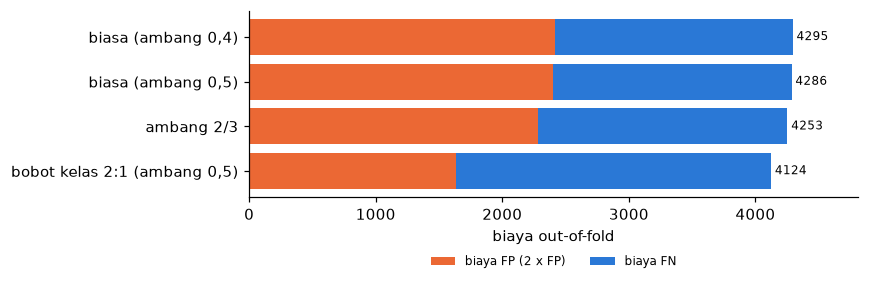
\includegraphics[width=0.85\textwidth]{dtl/dtl_cost_sensitive.png}
	\caption{Komposisi total biaya OOF setiap skema: biaya FP ($2 \times FP$) dan biaya FN}
	\label{fig:cost-sensitive}
\end{figure}

\paragraph{\textit{Threshold moving} hampir tidak berpengaruh.} Menggeser \textit{threshold} dari 0,5
ke $2/3$ hanya menurunkan biaya dari 4.286 menjadi 4.253 (0,8\%). Sebanyak 61 \textit{false positive}
hilang dan 89 \textit{false negative} bertambah. Pohon final memiliki daun yang sangat murni, sehingga
hanya sedikit pemesanan yang peluangnya berada di antara 0,5 dan $2/3$. Akibatnya, menggeser
\textit{threshold} di rentang ini hanya mengubah sebagian kecil prediksi.

\paragraph{Pembobotan kelas lebih efektif.} Dengan bobot 2 : 1, \textit{false positive} turun dari
1.202 menjadi 817, dengan tambahan 608 \textit{false negative}, dan total biaya turun menjadi 4.124.
Dibandingkan skema standar dengan \textit{threshold} 0,5, penurunannya 162 (3,8\%), hampir lima kali
penurunan dari \textit{threshold moving}. Pembobotan bekerja saat pelatihan, sehingga pohon membuat
pemecahan dan daun baru, bukan hanya menggeser keputusan pada daun yang sama. Harganya adalah Macro F1
yang turun 0,0142, karena Macro F1 tidak membedakan biaya kedua jenis kesalahan.

\paragraph{Keterbatasan.} Semua angka berasal dari satu \textit{seed} pembagian, dan bobot kelas hanya
diuji pada satu nilai (2 : 1, sesuai matriks biaya). Selisih biaya antara skema standar dan
\textit{threshold moving} (33) kecil, sehingga dapat berubah pada \textit{seed} lain.

Kedua tujuan memerlukan model yang berbeda. Submisi Kaggle tetap memakai model standar dengan
\textit{threshold} 0,4 karena kompetisi dinilai dengan Macro F1. Untuk penginapan yang memakai
prediksi ini untuk menjual ulang kamar, kami menyarankan model dengan pembobotan kelas 2 : 1, karena
model itu paling jarang salah menandai tamu yang sebenarnya datang.

\section{Submisi Kaggle}
\label{sec:kaggle}

\todo{Nama tim di \textit{leaderboard}, riwayat submisi penting, model dan konfigurasi submisi final, skor \textit{public}/\textit{private}, serta peringkat. Tegaskan bahwa model final adalah implementasi \textit{from scratch} tunggal tanpa \textit{ensemble}, dan sebutkan notebook yang mereproduksi skor tersebut.}

\begin{figure}[H]
	\centering
	\placeholdergambar{\textit{Screenshot leaderboard} Kaggle}
	\caption{Posisi kelompok pada \textit{leaderboard} Kaggle}
	\label{fig:kaggle}
\end{figure}

\section{Rekapitulasi Bonus}
\label{sec:rekap-bonus}

\todo{Isi status setiap bonus dan rujukan subbabnya agar mudah diperiksa asisten. Hapus baris bonus yang tidak dikerjakan.}

\begin{table}[H]
	\centering
	\caption{Rekapitulasi bonus yang dikerjakan}
	\label{tab:rekap-bonus}
	\begin{tabularx}{\textwidth}{l Y c}
		\toprule
		\textbf{Bonus} & \textbf{Keterangan} & \textbf{Subbab} \\
		\midrule
		Kaggle & Peringkat \textit{leaderboard} & \ref{sec:kaggle} \\
		DTL & Gambar percabangan pohon dengan \textit{top-N} & \ref{subsec:dtl-bonus} \\
		\textit{Logistic Regression} & Video kontur \textit{log-loss} & \ref{subsec:lr-bonus} \\
		SVM & Gambar bidang pemisah per kernel & \ref{subsec:svm-bonus} \\
		\textit{Naive Bayes} & Graf \textit{Bayesian network} & \ref{subsec:nb-bonus} \\
		Optimasi model & Algoritma di luar materi kelas & \todo{} \\
		\textit{Cost-sensitive} & FP $2\times$ lebih mahal dari FN & \ref{sec:cost-sensitive} \\
		\bottomrule
	\end{tabularx}
\end{table}



	\chapter{Kesimpulan dan Saran}
	\section{Kesimpulan}
\label{sec:kesimpulan}

Berdasarkan implementasi dan eksperimen pada tugas ini, kesimpulan yang dapat ditarik adalah sebagai
berikut.

\begin{enumerate}
	\item Kelima algoritma, yaitu KNN, DTL (C4.5), \textit{Logistic Regression} dengan regularisasi L1,
	L2, dan \textit{Elastic Net}, SVM dengan kernel \textit{linear}, \textit{polynomial}, dan
	\textit{Gaussian}, serta \textit{Naive Bayes}, berhasil diimplementasikan \textit{from scratch}.
	Setiap model dapat disimpan dan dimuat kembali.
	\item Pada protokol pembanding yang sama, KNN, \textit{Logistic Regression}, SVM, dan \textit{Naive
	Bayes} \textit{from scratch} menghasilkan Macro F1 yang sama dengan \textit{scikit-learn} sampai
	empat desimal, dengan selisih terbesar 0,0003. DTL C4.5 \textit{from scratch} lebih tinggi daripada
	konfigurasi \texttt{DecisionTreeClassifier} terbaik (0,8692 berbanding 0,8642) karena memakai
	\textit{gain ratio}, pemecahan kategorikal multicabang, penanganan nilai kosong dengan bobot
	fraksional, dan \textit{pruning}.
	\item Model terbaik adalah SVM dengan kernel yang dipelajari, dengan Macro F1 validasi silang 0,8750 (satu
	\textit{seed}) dan skor \textit{public} Kaggle 0,87912 (0,87973 untuk varian 255 kuantil). SVM dengan kernel Laplacian dan bobot fitur mendapat
	0,8703 dan 0,87464, dan DTL mendapat 0,8670 dan 0,87393.
	\item Tahap \textit{preprocessing} yang paling berpengaruh adalah pembentukan fitur ``saudara'', yaitu
	informasi dari pemesanan lain yang mirip pada data latih. Fitur \texttt{sib\_te} menjadi pemecahan
	akar pohon DTL, dan keunggulan SVM atas pohon pembanding seluruhnya berasal dari baris yang memiliki
	saudara. Sebaliknya, PCA tidak membantu SVM sehingga tidak dipakai pada model akhir.
	\item Dengan asumsi FP dua kali lebih mahal daripada FN, penanganan yang tepat adalah mengurangi
	prediksi batal: menaikkan \textit{threshold} atau memberi bobot lebih besar pada kelas tidak batal.
	Pada DTL, pembobotan kelas 2 : 1 menurunkan total biaya OOF dari 4.286 menjadi 4.124, sedangkan
	pada KNN \textit{threshold} $2/3$ menurunkan biaya \textit{hold-out} sebesar 8,87\%. Pada kedua
	model, Macro F1 turun sebagai gantinya, sehingga model untuk penginapan sebaiknya dipilih berdasarkan
	biaya, bukan hanya Macro F1.
\end{enumerate}

\section{Saran}
\label{sec:saran}

Beberapa hal yang dapat dikembangkan lebih lanjut adalah sebagai berikut.

\begin{enumerate}
	\item Kesalahan terbanyak terjadi pada baris tanpa saudara di data latih (Macro F1 sekitar 0,81,
	dibandingkan sekitar 0,94 pada baris dengan saudara). \textit{Feature engineering} lanjutan untuk
	baris tersebut, misalnya fitur dari riwayat pelanggan atau pola musiman, kemungkinan memberi
	kenaikan yang lebih besar daripada \textit{tuning} model.
	\item SVM dan KNN mahal secara komputasi sehingga pemilihan konfigurasi SVM dilakukan pada sampel
	3.000 sampai 6.000 baris. Teknik \textit{shrinking} seperti pada LIBSVM, aproksimasi kernel
	(misalnya metode Nyström), atau struktur indeks tetangga (misalnya KD-tree) dapat memungkinkan
	pemilihan konfigurasi pada seluruh data.
	\item TAN sudah lebih baik daripada \textit{Naive Bayes}, tetapi setiap fitur hanya boleh memiliki
	satu \textit{parent} selain kelas. Struktur \textit{Bayesian network} yang lebih umum, misalnya hasil
	pencarian struktur berbasis skor, dapat dieksplorasi.
	\item Validasi \textit{cost-sensitive} sebaiknya memakai biaya nyata dari penginapan, karena rasio
	2 : 1 pada tugas ini adalah asumsi. \textit{Threshold} juga perlu dikalibrasi ulang jika rasio
	pembatalan pada data baru berubah.
\end{enumerate}


	\chapter{Pembagian Tugas}
	\todo{Isi nama, NIM, dan tugas tiap anggota. Pembagian ini juga harus dicantumkan di
\texttt{README.md}.}

\begin{table}[H]
	\centering
	\caption{Pembagian tugas anggota kelompok}
	\label{tab:pembagian-tugas}
	\begin{tabularx}{\textwidth}{l l Y}
		\toprule
		\textbf{NIM} & \textbf{Nama} & \textbf{Tugas} \\
		\midrule
		NIM & Nama Anggota 1 & \todo{} \\
		NIM & Nama Anggota 2 & \todo{} \\
		NIM & Nama Anggota 3 & \todo{} \\
		NIM & Nama Anggota 4 & \todo{} \\
		NIM & Nama Anggota 5 & \todo{} \\
		\bottomrule
	\end{tabularx}
\end{table}


	\bibliographystyle{ieeetr}
	\bibliography{dafpus}
	\addcontentsline{toc}{chapter}{Daftar Pustaka}

	\appendix
	\chapter{Tautan Penting}
\label{app:tautan}

\begin{table}[H]
	\centering
	\begin{tabularx}{\textwidth}{l Y}
		\toprule
		\textbf{Item} & \textbf{Tautan} \\
		\midrule
		\textit{Repository} GitHub & \url{https://github.com/MAJIIDMN/IF3170_G04_TreeIsAllYouNeed} \\
		\textit{Release} & \todo{tautan release vX.Y} \\
		Kompetisi Kaggle & \url{https://www.kaggle.com/t/f1501c0f1c234e5eabe5b479e7ced777} \\
		Video bonus LR & \todo{} \\
		\bottomrule
	\end{tabularx}
\end{table}

\chapter{Form Penggunaan \textit{Generative AI}}
\label{app:genai}

\todo{Lampirkan form penggunaan \textit{Generative AI} (halaman 19 Panduan AI ITB) yang diisi
dengan jujur. Form dapat ditulis ulang sebagai tabel di bawah, atau berkas PDF hasil
\textit{scan} disisipkan dengan \texttt{\textbackslash usepackage\{pdfpages\}} dan
\texttt{\textbackslash includepdf}.}

\begin{longtable}{p{3cm} p{4cm} p{7cm}}
	\toprule
	\textbf{Tools} & \textbf{Bagian pekerjaan} & \textbf{Bentuk penggunaan} \\
	\midrule
	\endhead
	\todo{} & & \\
	\bottomrule
\end{longtable}



\end{document}
